% \documentclass[12pt]{book}
\documentclass[a4paper,12pt]{report}
\usepackage[left=2.5cm,right=2cm,top=2cm,bottom=2cm]{geometry}

%%%%%%%%%%%%%%%%%%%%%%%%%%%%%%%%%%%%%%%%%%%%%%%%%%%%%%%%%%%%%%%%%%%%%
%				    PAKETA-FONTS									%
%%%%%%%%%%%%%%%%%%%%%%%%%%%%%%%%%%%%%%%%%%%%%%%%%%%%%%%%%%%%%%%%%%%%%
\usepackage{xltxtra} 
\usepackage{xgreek}
\usepackage{amssymb}
\usepackage{mathtools}
\usepackage{amsmath}
\usepackage{relsize}
\usepackage{array}
\usepackage{amsthm}
\usepackage{fancyhdr}
\usepackage{enumitem}
\usepackage{listings}
\usepackage{color}
\usepackage{pxfonts}
\usepackage{fontspec}
\usepackage{import}
\usepackage{imakeidx}
\usepackage{tikz}
\usetikzlibrary{arrows,shapes,positioning,calc}
%\usepackage[toc]{glossaries}
\usepackage[normalem]{ulem}
%\usepackage{ulem}
%\usepackage{hyperref}
\usepackage{setspace}
\usepackage{parskip}
\usepackage{caption}
\usepackage{subcaption}
\usepackage{float}


\setstretch{1.5}

\graphicspath{{images/}}

\renewcommand{\contentsname}{Table of Contents}
%%%%%%%%%%%%%%%%%%%%%%%%%%%%%%%%%%%%%%%%%%%%%%%%%%%%%%%%%%%%%%%%%%%%%
%					         Markdown	     						%
%%%%%%%%%%%%%%%%%%%%%%%%%%%%%%%%%%%%%%%%%%%%%%%%%%%%%%%%%%%%%%%%%%%%%

%\usepackage{markdown}

%n TeXStudio, click on the following menu

%Options > Configure TeXStudio > Commands

%and change

%pdflatex -synctex=1 -interaction=nonstopmode %.tex

%into

%pdflatex -synctex=1 -interaction=nonstopmode --shell-escape %.tex

%%%%%%%%%%%%%%%%%%%%%%%%%%%%%%%%%%%%%%%%%%%%%%%%%%%%%%%%%%%%%%%%%%%%%
%					Start View of the PDF							%
%%%%%%%%%%%%%%%%%%%%%%%%%%%%%%%%%%%%%%%%%%%%%%%%%%%%%%%%%%%%%%%%%%%%%
%\hypersetup{pdfstartview={XYZ null null 1.50}}
%1.00=100% 2.00=200%

%%%%%%%%%%%%%%%%%%%%%%%%%%%%%%%%%%%%%%%%%%%%%%%%%%%%%%%%%%%%%%%%%%%%%
%							configure GLOSSARY						%
%%%%%%%%%%%%%%%%%%%%%%%%%%%%%%%%%%%%%%%%%%%%%%%%%%%%%%%%%%%%%%%%%%%%%
%%%\usepackage[toc]{glossaries} % [toc] to show in toc
%\makeglossaries % to make a glossary
%%%\printglossary[title=Γνωστές Συναρτήσεις, toctitle=Γνωστές Συναρτήσεις] % for title and toc title
%%% makeglossaries filename (χωρις επεκταση) ή "filename" αν εχει κενα (χωρις επεκταση) at the terminal!!!
%\gls{ }
%To print the term, lowercase. For example, \gls{maths} prints mathematics when used.
%\Gls{ }
%The same as \gls but the first letter will be printed in uppercase. Example: \Gls{maths} prints Mathematics
%\glspl{ }
%The same as \gls but the term is put in its plural form. For instance, \glspl{formula} will write formulas in your final document.
%\Glspl{ }
%The same as \Gls but the term is put in its plural form. For example, \Glspl{formula} renders as Formulas.

%%%%%%%%%%%%%%%%%%%%%%%%%%%%%%%%%%%%%%%%%%%%%%%%%%%%%%%%%%%%%%%%%%%%%
%							GLOSSARY ENTRIES						%
%%%%%%%%%%%%%%%%%%%%%%%%%%%%%%%%%%%%%%%%%%%%%%%%%%%%%%%%%%%%%%%%%%%%%
%\newglossaryentry{rand()}
%{
	%	name=rand(),
	%	description={Εμφανίζει τυχαίους αριθμούς \index{rand()}}
	%}

%\newglossaryentry{maths}
%{
	%	name=mathematics,
	%	description={Mathematics is what mathematicians do \index{thisInGlos} }
	%}
%%%%%%%%%%%%%%%%%%%%%%%%%%%%%%%%%%%%%%%%%%%%%%%%%%%%%%%%%%%%%%%%%%%%%
%							configure INDEX							%
%%%%%%%%%%%%%%%%%%%%%%%%%%%%%%%%%%%%%%%%%%%%%%%%%%%%%%%%%%%%%%%%%%%%%
\makeindex[columns=1, title=Ευρετήριο,options= -s myStyleIndex.ist, intoc]

% in the document place \index{word}. The word will be in Index and not appear in document
%\printindex to the end of document to print Index there. 
%\index{keywords!used}. for subentries
%intoc for place Index in Toc
% make file myStyle.ist in the same folder to customize.
%Style files contain a list of <key, value> pairs. add to makeindex the -> options= -s myStyle.ist <-
% -s: To use style in the document 
%headings_flag = 1 enables grouping inserting the group header (symbols, numbers or letters) before a new group.
%heading_prefix formats the header to insert before a new letter begins. It customize the Header of a group.
%delim_* is the delimiter to be inserted between the key and the first page number.

%%%%%% IN order to work you must run in cmd makeindex filename.idx
%%%%%%		IF filename has spaces Put it in "file name.idx"

%%%%put package \usepackage[xindy]{imakeidx} for support different characters beyond ASCII (for greeks)
\newfontfamily\listingsfont[Scale=0.8]{Courier New}
%\newfontfamily\listingsfont[Scale=0.8]{Segoe UI}
%\newfontfamily\listingsfont[Scale=0.8]{Monoid}

%%%%%%%%%%%%%%%%%%%%%%%%%%%%%%%%%%%%%%%%%%%%%%%%%%%%%%%%%%%%%%%%%%%%%
%				configure listing properties						%
%%%%%%%%%%%%%%%%%%%%%%%%%%%%%%%%%%%%%%%%%%%%%%%%%%%%%%%%%%%%%%%%%%%%%
\lstset{
	aboveskip=3mm,
	belowskip=3mm,
	frame=single,
	%framexleftmargin=10mm,
	%framexrightmargin=0mm,
	%framerule=1.8pt,
	%rulesep=10pt,
	%frameround=tttt,
	%xleftmargin=0em,
	%framesep=10mm,
	rulecolor=\color{pythonRuleLightGrey},
	%numbersep=0pt,
	showstringspaces=false,
	columns=fixed,
	basicstyle=\small\listingsfont,
	numbers=left,
	language=Python,
	numberstyle=\color{black},
	keywordstyle=\bfseries\color{pythonMagenta},
	commentstyle=\color{pythonCommentBlack},
	stringstyle=\color{pythonGreen},
	breaklines=true,
	breakatwhitespace=false,
	tabsize=4,
	backgroundcolor =\color{lightgray}
}
%%%%%%%%%%%%%%%%%%%%%%%%%%%%%%%%%%%%%%%%%%%%%%%%%%%%%%%%%%%%%%%%%%%%%
%							LIST STYLES								%
%%%%%%%%%%%%%%%%%%%%%%%%%%%%%%%%%%%%%%%%%%%%%%%%%%%%%%%%%%%%%%%%%%%%%

%%%%%%%%%%%%%%%%%%%%%%%%%%%%%%%%%%%%%%%%%%%%%%%%%%%%%%%%%%%%%%%%%%%%%
%							CAPTION									%
%%%%%%%%%%%%%%%%%%%%%%%%%%%%%%%%%%%%%%%%%%%%%%%%%%%%%%%%%%%%%%%%%%%%%
\renewcommand{\lstlistingname}{Code}
\renewcommand{\lstlistlistingname}{Codes}

%%%%%%%%%%%%%%%%%%%%%%%%%%%%%%%%%%%%%%%%%%%%%%%%%%%%%%%%%%%%%%%%%%%%%
%							COLORS									%
%%%%%%%%%%%%%%%%%%%%%%%%%%%%%%%%%%%%%%%%%%%%%%%%%%%%%%%%%%%%%%%%%%%%%
\definecolor{purple}{rgb}{0.58, 0.0, 0.33}
\definecolor{green}{rgb}{0.25, 0.5, 0.37}
\definecolor{black}{rgb}{0.0,0.0,0.0}
\definecolor{blue}{rgb}{0.33, 0.0, 1.0}
\definecolor{lightgray}{rgb}{0.95, 0.95, 0.95}
\definecolor{red}{rgb}{0.9, 0.0, 0.0}

\definecolor{pythonOrange}{rgb}{0.96, 0.53, 0.12}
\definecolor{pythonBlue}{rgb}{0.26, 0.44, 0.68}
\definecolor{pythonMainBlack}{rgb}{0.30, 0.30, 0.30}
\definecolor{pythonCommentBlack}{rgb}{0.56, 0.56, 0.56}
\definecolor{pythonGreen}{rgb}{0.44, 0.55, 0.0}
\definecolor{pythonMagenta}{rgb}{0.54, 0.35, 0.66}
\definecolor{pythonBackgroundLightGrey}{rgb}{0.97, 0.97, 0.97}
\definecolor{pythonRuleLightGrey}{rgb}{0.80, 0.80, 0.80}

%%%%%%%%%%%%%%%%%%%%%%%%%%%%%%%%%%%%%%%%%%%%%%%%%%%%%%%%%%%%%%%%%%%%%
%							TIKZ STYLE								%
%%%%%%%%%%%%%%%%%%%%%%%%%%%%%%%%%%%%%%%%%%%%%%%%%%%%%%%%%%%%%%%%%%%%%

\tikzstyle{boxtrapezium} = [trapezium,trapezium right angle=110,trapezium left angle=-110, minimum width=3cm, minimum height=2cm, text centered, draw=black, fill=white]
\tikzstyle{box} = [rectangle, minimum width=3cm, minimum height=2cm, text centered, draw=black, fill=white]
\tikzstyle{boxheight} = [rectangle, minimum width=1cm, minimum height=2cm, text centered, draw=black, fill=white]
\tikzstyle{littlebox} = [rectangle, minimum width=0.7cm, minimum height=0.7cm, text centered, draw=black, fill=white]
\tikzstyle{arrow} = [thick,->,>=stealth]
\tikzstyle{arrowLine} = [very thick]
\tikzstyle{nobox} = [rectangle, minimum width=3cm, minimum height=2cm, text centered, draw=white, fill=white]
\tikzstyle{smallbox} = [rectangle, minimum width=3cm, minimum height=1cm, text centered, draw=black, fill=white,node distance=3cm]
\tikzstyle{linkedlistnode} = [rectangle, minimum width=2cm, minimum height=1cm, text centered, draw=black, fill=white,node distance=0.5cm,outer sep=0cm]
\tikzstyle{ptrlinkedlistnode} = [rectangle, minimum width=1cm, minimum height=1cm, text centered, draw=black, fill=white,node distance=0cm,outer sep=0cm]
\tikzstyle{circleNode} = [circle, ultra thick, minimum size=1cm, text centered, draw=black, fill=white]
%\tikzstyle{linkedlistnode}=[rectangle split, rectangle split horizontal, rectangle split parts=2, inner xsep=1cm, draw=black, fill=white, text centered]


\newcommand{\tikzmark}[1]{\tikz[overlay,remember picture] \node (#1) {};}


%%%%%%%%%%%%%%%%%%%%%%%%%%%%%%%%%%%%%%%%%%%%%%%%%%%%%%%%%%%%%%%%%%%%%
%				klisi entolwn gia global scope						%
%%%%%%%%%%%%%%%%%%%%%%%%%%%%%%%%%%%%%%%%%%%%%%%%%%%%%%%%%%%%%%%%%%%%%

%\setmainfont[
%  ItalicFont={GFS Didot Italic},
%  BoldFont={GFS Didot Bold},
%  BoldItalicFont={GFS Didot Bold Italic},
%]{GFS Didot}
%\theoremstyle{definition} %allazoume to style tou environment theorem (ta tria styles einai: plain definition remark)
\newtheoremstyle{definitionNODot}
{\topsep}                % Space above
{\topsep}                % Space below
{\normalfont}        % Theorem body font % (default is "\upshape")
{0pt}                % Indent amount
{\bfseries}       % Theorem head font % (default is \mdseries)
{}               % Punctuation after theorem head % default: no punctuation
{5pt plus 1pt minus 1pt}               % Space after theorem head
{}                % Theorem head spec
\theoremstyle{definitionNODot}
\newtheorem{theorem}{Theorem}
\setmainfont[Ligatures=TeX]{Calibri} %vazoume ti grammatoseira
\setlength{\parindent}{0.75cm} %edw tou leme oti den theloume keno otan arxizei i kainouria paragrafos
\setcounter{chapter}{0} %edw vazoume ton metriti apo to miden
%\pagestyle{fancy} % (usepackage {fancyhdr} edw orizoume to style tin selidas) 
\fancyhead{} %katharizoume oti header exoun oi selides
\setlength{\headheight}{15pt}
\fancyhead[RE,LO]{\leftmark} % L=left R=right C=centered O=odd E=even H=header F=footer
\pagestyle{plain}
%%%%%%%%%%%%%%%%%%%%%%%%%%%%%%%%%%%%%%%%%%%%%%%%%%%%%%%%%%%%%%%%%%%%%
%		 Orismoi sundiasmwn grammato-entolwn		  			    %
%%%%%%%%%%%%%%%%%%%%%%%%%%%%%%%%%%%%%%%%%%%%%%%%%%%%%%%%%%%%%%%%%%%%%


%%%%%%%%%%%%%%%%%%%%%%%%%%%%%%%%%%%%%%%%%%%%%%%%%%%%%%%%%%%%%%%%%%%%%
%				Orismoi thewrimatwn									%
%%%%%%%%%%%%%%%%%%%%%%%%%%%%%%%%%%%%%%%%%%%%%%%%%%%%%%%%%%%%%%%%%%%%%
%	exw class-object theorem new theorem
%	{environment name}{header tect} edw to counter dimiourgite me to 
%		onoma tou environment automata
%	anamesa sto prwto kai to deutero mporw na valw [section] edw tha mirazetai to counter tou section
%   an to valw sto telos to [section] tha metraei kathe fora MESA se kathe section diladi otan arxizei ena section
%		arxizei kai to metrima ara ousiastika exei to diko tou counter aneksartita apo to section
%	otan to valw anamesa apo ta duo {}[ thewrima] {} tha mirazete to counter tou thewrima-environment

\newtheorem{thewrima}{Θεώρημα}[section]
\newtheorem{limma}[thewrima]{Λήμμα}
\newtheorem{protasi}[thewrima]{Πρόταση}
\newtheorem{porisma}[thewrima]{Πόρισμα}
\newtheorem{orismos}[thewrima]{Ορισμός}
\newtheorem*{paratirisi*}{Παρατήρηση}
\newtheorem{paratiriseis}[thewrima]{Παρατηρήσεις}
\newtheorem{isxurismos}[thewrima]{Ισχυρισμός}
\newtheorem{sxolio}[thewrima]{Σχόλιο}
\newtheorem{paradeigma}[thewrima]{Παράδειγμα}
\newtheorem{paradeigmata}[thewrima]{Παραδείγματα}
\newtheorem{upothesi}[thewrima]{Υπόθεση}
\newtheorem{askisi} {} 
\newtheorem{eikasia}[thewrima]{Εικασία}
\newtheorem*{leksi}{}

\newenvironment{block}{
	
}

%%%%%%%%%%%%%%%%%%%%%%%%%%%%%%%%%%%%%%%%%%%%%%%%%%%%%%%%%%%%%%%%%%%%%
%				Orismoi Operator									%
%%%%%%%%%%%%%%%%%%%%%%%%%%%%%%%%%%%%%%%%%%%%%%%%%%%%%%%%%%%%%%%%%%%%%

%\DeclareMathOperator{\Int}{int}
%\DeclareMathOperator{\cl}{cl}

%%%%%%%%%%%%%%%%%%%%%%%%%%%%%%%%%%%%%%%%%%%%%%%%%%%%%%%%%%%%%%%%%%%%%
%				Orismoi entolwn gia metro kai apoluta 				%
%%%%%%%%%%%%%%%%%%%%%%%%%%%%%%%%%%%%%%%%%%%%%%%%%%%%%%%%%%%%%%%%%%%%%
%\newcommand{\abs}[1]{\left\lvert#1\right\rvert} % absolute value: single vertical bars
%\newcommand{\norm}[1]{\left\lVert#1\right\rVert} % norm: double vertical bars

%%%%%%%%%%%%%%%%%%%%%%%%%%%%%%%%%%%%%%%%%%%%%%%%%%%%%%%%%%%%%%%%%%%%%
%					Change Tabular (array) Row Height 				%
%%%%%%%%%%%%%%%%%%%%%%%%%%%%%%%%%%%%%%%%%%%%%%%%%%%%%%%%%%%%%%%%%%%%%
\renewcommand{\arraystretch}{2}
% gia na mpei centered ston pinaka (an den mpei auto me to p(2cm) mpainei align left automata)
\newcolumntype{P}[1]{>{\centering\arraybackslash}p{#1}}
%%%%%%%%%%%%%%%%%%%%%%%%%%%%%%%%%%%%%%%%%%%%%%%%%%%%%%%%%%%%%%%%%%%%%
% Allagi arithmisis apo (1,2,3) se Roman (i,ii,iii) gia ta ITEMS	%
%%%%%%%%%%%%%%%%%%%%%%%%%%%%%%%%%%%%%%%%%%%%%%%%%%%%%%%%%%%%%%%%%%%%%

%\arabic (1, 2, 3, ...)
%\alph (a, b, c, ...)
%\Alph (A, B, C, ...)
%\roman (i, ii, iii, ...)
%\Roman (I, II, III, ...)
%\fnsymbol (∗, †, ‡, §, ¶, ...)
\renewcommand\thepart{\Roman{part}}

\renewcommand*{\proofname}{Απόδειξη}  % allazei to proof stin apodeiksi se "Απόδειξη"
\renewcommand*{\chaptername}{Chapter}  % allazei to "κεφαλαιο" se "Μάθημα"
\renewcommand\labelenumi{(\roman{enumi})} % allagi tis arithmisis apo (1,2,3)
\renewcommand\theenumi\labelenumi % se (i,ii,iii) twn items twn listwn.
\renewcommand{\qedsymbol}{} %allazei to simvolo stin apodeiksh anti gia adio tetragwno vazei tipota.
\renewcommand*{\appendixname}{MyAppx}
%%%%%%%%%%%%%%%%%%%%%%%%%%%%%%%%%%%%%%%%%%%%%%%%%%%%%%%%%%%%%%%%%%%%%
%				Titlos-Prwti selida									%
%%%%%%%%%%%%%%%%%%%%%%%%%%%%%%%%%%%%%%%%%%%%%%%%%%%%%%%%%%%%%%%%%%%%%
\makeatletter
\def\maketitle{
	\begin{titlepage}{
			\begin{center}
				\begingroup
				\fontsize{18pt}{12pt}\selectfont
				HAROKOPIO UNIVERSITY
				
				SCHOOL OF DIGITAL TECHNOLOGY
				
				DEPARTMENT OF INFORMATICS AND TELEMATICS
				\endgroup
				
				\begingroup
				\fontsize{16pt}{12pt}\selectfont
				POSTGRADUATE PROGRAM INFORMATICS AND TELEMATICS
				
				COURSE WEB TECHNOLOGIES AND APPLICATIONS
				\endgroup
				\rm
				\vskip 2.5in
				
				\begingroup
				\fontsize{14pt}{12pt}\selectfont
				\bf \@title \par
				\endgroup
				
				\begingroup
				\fontsize{14pt}{12pt}\selectfont
				Master Thesis
				\endgroup			
			\end{center}
			
		}
		\begin{center}
			\vskip 0.3in
			
			\begingroup
			\fontsize{14pt}{12pt}\selectfont
			by
			\vskip 0.3in
			\@author
			
			\vspace*{\fill}
			
			Athens, 2023
			\endgroup	
			
		\end{center}
	\end{titlepage}
}
\def\makeabstract{
	%\pagestyle{empty}
	
	
	\section*{Abstract}
	\addcontentsline{toc}{chapter}{Abstract}
	\noindent 
	Anomaly Detection in multivariate time series is a major problem in many fields. As the number of anomalies in real data is much smaller than the size of data it is difficult problem for categorization algorithms to solve. Also due to the variety of anomalies it is necessary to be used algorithms specially designed corresponding to the specific type of anomalies. Basic methods based on Deep Learning such as LSTM, Autoencoder, Convolutional-Autoencoder, have shown positive results in anomaly detection. The major challenge algorithms face when they applied to multivariate time series, relies on the fact that the anomaly can arise from one feature or a small subset of the total features. The detection is done based on a dynamic threshold which compared with Anomaly Score that the algorithm assign to every point. If the Anomaly Score is greater than the threshold then the point is labeled as anomalous otherwise it is labeled as normal. In order to increase effectiveness, we use ensemble techniques based on these (basic) algorithms. We apply the Majority Voting technique where five algorithms are used and the result concluded based on the majority (every vote has a weight of 1). Then we apply a variation of Majority Voting where a semi-supervised learning is done and in the final stage a Logistic Regressor is responsible to combine the basic algorithms. Also we use the idea of Feature Bagging taken from Random Forests, adjusted on time series data for the anomaly detection problem and extended using the method PCA to rotate the space so that the models can more easily identify anomalies. We call this method Feature Bagging with Rotation. Finally we will create models using the technique of Feature Bagging with Rotation and we will apply the Stacking method with a Logistic Regressor as meta-learner. The results are mixed and there is not a solution that fits all. However, results prove that ensemble techniques have better performance in many cases than the basic algorithms. More specific, the algorithm using Feature Bagging with Rotation performs better than the basic models and achieves up to 2 \% better results. If we apply stacking on models that created with Feature Bagging with Rotation, with Logistic Regressor as meta-learner, performance is raised up to 10 \%. The data that we used are datasets from the SKAB (Skoltech Anomaly Benchmark), which contain anomalies that have been generated to simulate different conditions.
	
	\vfil
	
	\noindent \textit{keywords}: Anomaly Detection, Ensemble, Deep Learning, Time Series, Multivariate
	
	
	\newpage
}
\makeatother
\title{Anomaly detection on multivariate time series using ensemble techniques}
\author{Anastasios Iliopoulos}
\date{\today}



%%%%%%%%%%%%%%%%%%%%%%%%%%%%%%%%%%%%%%%%%%%%%%%%%%%%%%%%%%%%%%%%%%%%%
%				APO EDW ARXIZOUME									%
%%%%%%%%%%%%%%%%%%%%%%%%%%%%%%%%%%%%%%%%%%%%%%%%%%%%%%%%%%%%%%%%%%%%%

\begin{document}
	\pagenumbering{roman}
	\maketitle
	{
		%\pagestyle{empty}
		\tableofcontents
		\cleardoublepage
	}
	\pagenumbering{arabic}
	\setcounter{page}{1}
	\makeabstract
	
	
	
	\chapter{Introduction}
	%\markboth{Εισαγωγή}{Εισαγωγή} %gia na mpei sto header tis kathe selidas kai sta ziga kai sta mona (BOTH) mono sta ziga (markeven h markright kati tetoio). gia na mpei sta aristera{Εισαγωγή} gia na mpei sta deksia {Εισαγωγή} (otan lew gia nampei aristera - deksia ennow ekei pou mpainei kati sta deksia sto sigkekrimeno to exw kanei na mpainei deksia-titlos-tou chapter-sta ziga-na mpainei sta deksia panw)
	%\addcontentsline{toc}{chapter}{Εισαγωγή} %vazw sto toc (table of contents) me to argument {toc} to chapter me to arg {chapter} tin leksi Εισαγωγή me to arg {Εισαγωγή}
	\section{Machine Learning, Time Series and Anomaly Detection}
	Machine learning is a subfield of statistics. Through the use of statistical methods, algorithms are trained on historical data to make predictions. Other applications that machine learning is used are classification, value prediction and clustering.
	
	Training can take several forms and some of them characterize the nature of training. We apply supervised learning when we supply the model with labels. The model trained in order to be able to predict these labels. In supervised learning we tell the model to find any relationship exists between the input data and labels. Another form of training is unsupervised learning which is exactly the opposite from the previous form. Model never gets the labels so it is required to find the patterns between data without any knowledge of the desired outcome. Semi-supervised learning is επαινοςcalled a form that lies between the previous two. In this form a part of labels supplied to the model. Finally the reinforcement learning refers to a form in which the model interact with an environment. When the model does a desired action then we reward it, otherwise we penalize it. The goal of the model is to earn as many points of reward as it can.
	
	While a model get historical data as input, the model compute parameters/variables named weights. So this process is called training and we say that the model is learning. When the model finish this process it means that it has computed every weight so it is capable of making predictions in new data. After training the model may be overfitted or underfitted or well generalized. A model is called overfitted if it is aligned to the training data, but when we feed it with new data it generates big errors. On the other hand, underfitted is called a model if it is unable to capture any relationship as a result it generates again big errors. The ideal scenario for a model is to be generalized which means it never generates errors or at least they are really small and is closer to the desired output. To explain better these terms lets give an example. Consider a student that is going to give an exam. Lets assume that the student memorize every past exam but he didn't understand or learn anything. If the student face a different problem than those he memorized then the student will not pass the exam. So the student is overfitted. On the other hand if the student didn't study then he will not pass the exam again. So in this situation we say that the student is underfitted. Generally we want our models to be generalized in order to learn the relationships between data and be able to perform well in any new data. 
	
	Deep Learning is a subfield of machine learning and is the field that study the neural networks. The most simple neural network is a network that consists of some neurons in successive layers, it is call Feed Forward Neural Network and it is used in the context of supervised classification problem. Let $\mathcal{X}$ be a set of data where every element $X$ is in the form of $X=(x_1,x_2,...,x_n)$ and let $\mathcal{L}=\left \{l_1,l_2,....,l_k \right \}$ the set of labels such that every element of this set $X\in\mathcal{D}$ maps to $X_i \mapsto l_j$. Then we define $z=w_1\cdot x_1 + w_2\cdot x_2 +...+w_n\cdot x_n + b \Rightarrow Z = W^T \cdot X + B$. Next we apply a function (which is called activation function) $h$. Finally we will get the prediction $\hat{y} = h(z)$. If instead of the output add another round of computations (or many more rounds) and after that we add the output layer then these layers (rounds) called hidden layers Σχ.~\ref{fig:neural_networks}. 
	
	\begin{figure}[h]
		\begin{subfigure}[b]{0.33\textwidth}
			\centering
			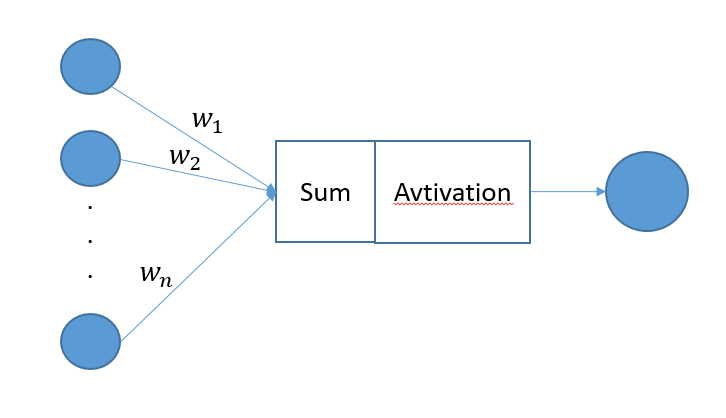
\includegraphics[width=\textwidth]{single.png}
			\caption{Input - Output}
			\label{fig:single}
		\end{subfigure}
		\hfill
		\begin{subfigure}[b]{0.49\textwidth}
			\centering
			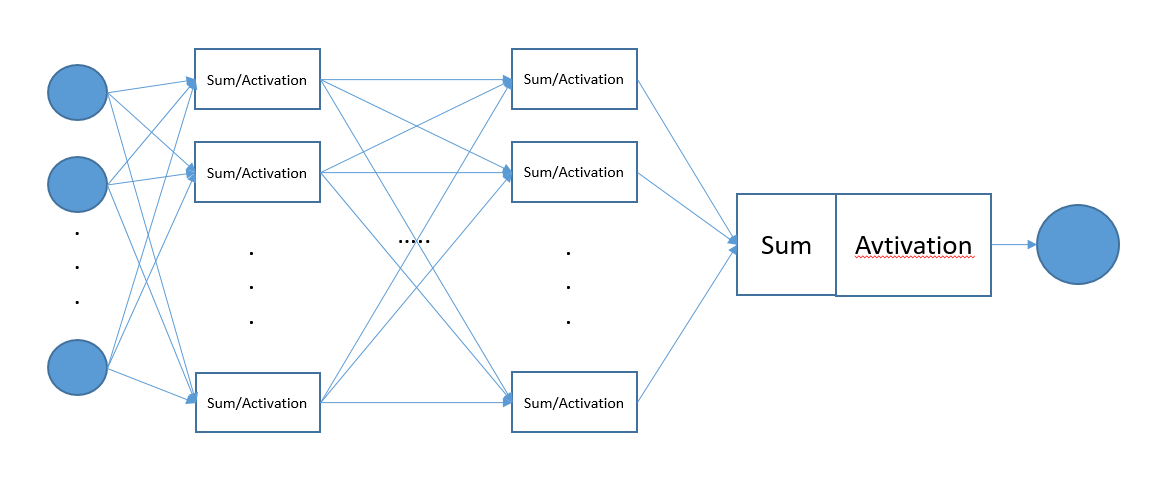
\includegraphics[width=\textwidth]{multiple.png}
			\caption{Multiple Hidden Layers}
			\label{fig:multiple}
		\end{subfigure}
		\caption{Neural Networks}
		\label{fig:neural_networks}
	\end{figure}
	
	Time series is a term that is defined as a sequence of values indexed with time. Machine learning can used in the context of time series to predict the next value in the future. Other applications regarding time series are classification in which model tries to classify a time series or a part of it and clustering in which model tries to group the data. Another application of using machine learning on time series data is the anomaly detection. In essence, much of real data is represented through time series which is data from systems, phenomena, or organs. If during the evolution (regarding time) of an operation, phenomenon or process there is something wrong then we get an anomaly. Then it is vital to get these points (anomalous points), and automatically recognize if a value is anomaly or not.
	
	The increase in the amount of data makes it difficult for humans to detect anomalies, and that is why we use algorithms to make the detection efficient and fast. It is therefore necessary to find models that detect "abnormalities" during the evolution of a process. There are many problems that anomaly detection tries to solve such as detecting bank fraud or early detection of tool malfunctions. Other applications relate to the health sector, such as the detection of various diseases or viruses. Applications also exist in industry such as fault detection or the detection of incorrect operation of a machine. Also money transactions and general fraud detection lies under the anomaly detection. These are just a few of the examples we can give in relation to anomaly detection.
	
	\section{Time Series and Stochastic Processes}
	
	In the study of phenomena, values emerge that appear in time sequence, one after the other. This family is called time series and formally we write $ X(t), t\in \mathbb{R}$. If for each moment we get more than one value we say that we have a multivariate time series and it is denoted by $  (X_i)_t, \quad t\in \mathbb{R}, \quad i\in \mathbb{I} $ where $X_{i,t}$ is the $i$ component of $Χ$ in time $t$. Otherwise, if for every moment we get a single value times series is called univariate time series. For example if we have a sensor that gives us a values for a phenomenon then the result will be a univariate time series. On the hand if we have many sensors then the result will be a multivariate time series. Len $\Omega$ be a sample space, we say that the family $X(\omega,t) $ where $t\in\mathbb{R}, \quad \omega \in \Omega$ is a stochastic process and for a moment of time $t\in \mathbb{R} $ the $X_t( \omega )$ is a random variable \cite{wei2006time}.
	
	A time series is said to have \textbf{Trend} if its mean $\mu$ is not constant and it increases or decreases with time. Also it is said that it has \textbf{Seasonality} if there is a periodic repetition of its fluctuations and is usually observed on an annual or monthly basis. Let be a time sereis, we define autocorrelation $\rho_\tau$ for a lag $\tau$ and the correlation coefficient two
	elements of the time series that are $\tau$ time steps apart and is estimated from the time series as
	
	$$ \rho_\tau = \text{Corr}(x_t, x_{t+\tau}) = E[(x_t-\mu)(x_{t+\tau}-\mu)] $$
	
	\noindent and correlation coefficient
	
	$$ r_\tau=\frac{\rho_\tau}{\rho_0} \quad , \quad -1\leq\rho_\tau\leq1$$
	
	\noindent Correlation make sense if time series is stationary.
	
	A time series that has no trend (ie has a mean of 0), no seasonality, constant variance, and constant autocorrelation is called \textbf{Στάσιμη} \cite{hyndman2018forecasting}. Noise $\epsilon_t$ is a stochastic process that is uncorrelated with time and comes from a distribution with constant mean $\mu=0$ and finite variance. Thus noise is a stationary stochastic process.
	
	\section{The problem of Anomaly Detection}
	The goal of Machine Learning is to identify the abnormal points of a time series in the future so that the necessary actions can be taken, for example if it is a fault, the fault should be fixed, or if it is an illegal entry into a system it should be dealt with. To go deeper into this problem we must first define what an Anomaly is. The term Anomaly is not easy to define. Therefore, several attempts have been made to define this term. According to Hawkins \cite{hawkins1980identification} an Anomaly is "an observation that deviates so significantly from other observations as to arouse suspicion that it was produced by some other mechanism". Then comes the term outlier. Many do not distinguish between these two terms and consider them equivalent. Thus we have definitions such as Grubbs \cite{grubbs1969procedures} who says that "Outlier observations, or outliers, are those which appear to deviate significantly from the other members of the sample in which they occur". And finally we get Aggarwal's definition which combines the two definitions into one as follows "Outlying points are often also referred to as non-normal, inconsistent, abnormal or anomalous, in the Data Mining and Statistics Literature". We will consider the term Anomaly to be equivalent to the term Outlier point. Here we have to distinguish the term Anomaly from the term Novelty which refers to data that is acceptable but does not resemble the rest of our sample \cite{Singh2003Novelty}. However, most algorithms are used to find both, so no further distinction will be made here. Finally, the main and most important problem in the definition of Anomaly is the concept of Noise. Noise are points that lie on the border between normal data and Anomalies, which could be called anomalies but are not points of interest. For this reason it is difficult to distinguish them Fig.~\ref{fig:anomaly vs anomaly with noise}. Some give the definitions \textit{Strong Anomaly} and \textit{Weak Anomaly} \cite{knorr1999finding} to distinguish the two concepts.
	
	\begin{figure}[h]
		\begin{subfigure}[b]{0.49\textwidth}
			\centering
			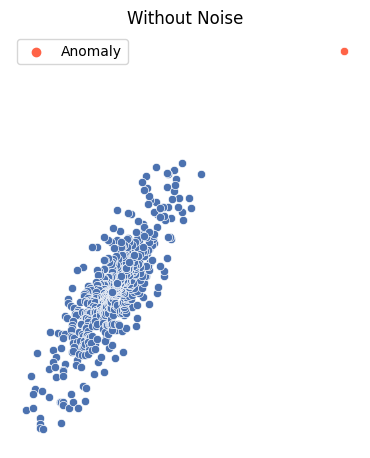
\includegraphics[width=\textwidth]{anomaly_vs_noise_clear_outlier.png}
			\caption{Anomaly without Noise}
			\label{fig:anomaly without noise}
		\end{subfigure}
		\hfill
		\begin{subfigure}[b]{0.49\textwidth}
			\centering
			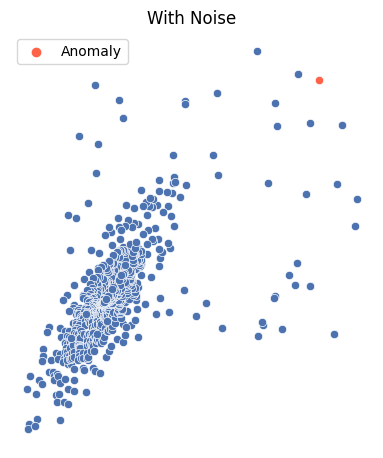
\includegraphics[width=\textwidth]{anomaly_vs_noise_no_clear_outlier.png}
			\caption{Anomaly with Noise}
			\label{fig:anomaly with noise}
		\end{subfigure}
		\caption{Anomaly with and without Noise}
		\label{fig:anomaly vs anomaly with noise}
	\end{figure}
	\noindent Thus, taking into account the above, we accept the following definition \cite{braei2020anomaly}:
	
	\begin{center}
		\textit{"An anomaly is an observation or sequence of observations that deviates significantly from the general distribution of the data. The total anomalies are a very small part of the total data."}
	\end{center}
	\hfill
	
	\section{Anomaly Types}
	
	Anomalies fall into three categories:
	
	\begin{itemize}
		\item \textbf{Point Anomalies} are called the points which deviate significantly from the rest of the sample. For example, a huge financial transaction that differs from the rest is called a Point Anomaly.
		
		\item \textbf{Collective Anomalies} are called the points which may be normal if we observe them individually but all together have an abnormal behavior. For example, if a customer of a bank withdraws 10 euros every 2 seconds from the bank, then these withdrawals are Collective Anomalies. 10 euros or 500 euros are normal amounts for a withdrawal but a series of such withdrawals is abnormal behavior.
		
		\item \textbf{Context Anomalies} or Context-dependent abnormalities are those points which are normal in a particular context but are reported as abnormal in another. For example the temperature $150 ^\circ C$ is a normal temperature for someone to cook their food in an oven but it is an abnormal value for the weather of a country.
	\end{itemize}
	
	\section{Anomaly Detection}
	
	Having defined what is an Anomaly, we can talk about Anomaly Detection. We define a function $ \varphi $ such that:
	\begin{align*}
		\varphi \colon \mathbb{R}^n \rightarrow \mathbb{R} \\
		\varphi(x)\mapsto\gamma
	\end{align*}
	where $ \gamma $ is Anomaly Score, $ x \in X \subseteq \mathbb{R}^n $ and $ X $ is the data set. Anomaly Score is defined as the measure to describe how much anomalous is a point, or how much this point deviates from the rest data set. We can transform it to a measure that belongs to interval $ [0,1] $ and then we can say that it is the probability of a point to be anomalous.
	
	To finally arrive at whether a point is an anomaly or not we define a threshold. A threshold is called a $ \delta \in \mathbb{R} $ , where all the points with an anomaly score below $ \delta $ will be the normal points while those with an anomaly score above $ \delta $ will be the anomalous points. Thus we define the binary anomaly detection method as:
	
	\begin{align*}
		\varphi_\text{binary} \colon \mathbb{R}^n \rightarrow \{Normal, Anomaly\} \quad \text{ή} \quad \{0,1\} \\
		\varphi_\text{binary}(x) \mapsto \begin{cases}
			Anomaly \quad \text{ή} \quad 1, & \text{if} \quad \varphi(x) > \delta \\
			\phantom{-}Normal \quad \text{ή} \quad 0, & \text{otherwise}
		\end{cases}
	\end{align*}
	
	Anomaly detection is not an ordinary two-class classification process. Naturally anomalies are less than 1\% which makes anomaly detection very different from two class classification. The difference lies in the fact that even if we say that all the points in a data set are normal points then the success of this model will be 99\%. But in reality the model will perform very poorly because it did not catch a single anomaly. For this reason we should tackle the problem with two well-known metrics: the F1 score and AUC (area under curve).
	
	$$ \text{Precision} = \frac{\text{TP}}{\text{TP}+\text{FP}}, \quad \text{Precision} = \frac{\text{TP}}{\text{TP}+\text{FN}} $$
	
	$$ \text{F}_1 = \frac{2 \cdot \text{Precision} \cdot \text{Recall}}{\text{Precision}+\text{Recall}} $$
	
	and
	
	$$ \text{TPR} = \frac{\text{TP}}{\text{TP}+\text{FN}}, \quad \text{FPR} = \frac{\text{FP}}{\text{FP}+\text{TN}} $$
	
	AUC is the area under the plot obtained by plotting on two vertical x,y axes, $ \text{FPR} $ on the x-axis and $ \text{TPR} $ on the y-axis. In essence, it shows how well the model can distinguish one class from another.
	
	Anomaly detection is not handled in the same way for all problems. Although we mentioned the difference in relation to two-class classification problems, we should say that anomaly detection problems (and thus their approaches) differ from each other depending on the type of anomalies they contain. This is clearly seen in the context of the time series we study in this thesis. For example, let's assume that we have a machine and we record in order among others the following temperatures in degrees Celsius: 35,34,34,35,36,37,36,90,92,92,93,92,94. If we approached the problem as if we had Point Anomalies then we probably wouldn't find any Anomalies because these temperatures are very normal for an engine. But if we take into account the time dependence of the temperatures then we observe an abnormal sudden rise from 36 degrees to 90. In the time series data we usually find Collective Anomalies or Anomalies that depend on the context (context anomalies).
	
	\chapter{Background}
	Anomaly detection is a subject that has many difficulties and is an evolving field. In the literature we will notice that the methods used can be categorized into 3 categories:
	
	\begin{itemize}
		\item Statistical methods
		\item Machine Learning methods
		\item Deep Learning methods
	\end{itemize}
	
	Statistical methods assume that anomalies generated from a statistical model. In contrast, in machine learning methods, the anomaly generation mechanism is considered as a black box and anomalies are detected based on the data. Finally, the third category concerns techniques based exclusively on neural networks, which are often considered part of Machine Learning, which is why there is often no separation between the second and third categories. Several methods have been presented by Markou, M. \& Singh, S. \cite{Singh2003Novelty, markou2003novelty} and by Chandola we have a very valuable research \cite{Chandola, chandola2009anomaly} who mentions algorithms of all three categories.
	
	\section{Statistical methods}
	
	\begin{itemize}
		\item \textbf{Autoregressive Model:}
		
		This model is considered linear where the value $X_t$ at time $t$ is based on the (finite) set of size $p$ of the previous values of the (stochastic) process and an error $\epsilon$, that is:
		
		$$X_t = \sum_{i=1}^{p}a_i X_{t-i} + c + \epsilon_t$$
		
		p is also called a window of length $p$ and the model is called an Autoregressive Model of order $p$ or simply $AR(p)$. The "error" values are considered uncorrelated and have mean $\mu=0$ and constant variance $\sigma$.
		
		The coefficients $a_1,....,a_p$ and $c$ can be approximated during training by solving the corresponding linear equations using the least square method. $\epsilon$ , which represents the anomaly score, can then be calculated as the difference between the "predicted" value and the actual value of X at time $t$ . The model assumes that the stochastic process is stationary, so if we do not have a stationary process then it should be transformed into one.
		
		\item \textbf{Moving Average Model:}
		
		While the previous model considers a $X_t$ value as a linear combination of the previous $p$ values, the Moving Average model considers this value as a linear combination of the previous $q$ forecasts' errors, so:
		
		$$X_t = \sum_{i=1}^{q}a_i \epsilon_{t-i} + \mu + \epsilon_t$$
		
		where $\mu$ is the mean value of X and the coefficients $a_1,....,a_q$ are calculated during training as before. $q$ is the size of the window and for this model (of order $q$) we write $MA(q)$. The difference with the previous model is that it considered the previous values from $X_t$ known, however in this model are considered unknown and predicted at each step thus producing the errors {$\epsilon_t,....\epsilon_{t-q}$}. 
		
		\item \textbf{Autoregressive Moving Average Model:}
		
		This model is a combination of the previous two and is often used on univariate time series data. denoted by $ARMA(p,q)$ and defined as:
		
		$$X_t = \sum_{i=1}^{p}a_i X_{t-i} + \sum_{i=1}^{q}b_i \epsilon_{t-i} + \epsilon_t$$
		
		$X(t)_{t\in\mathbb{R}}$ is an $ARMA(p,q)$ process if it is stationary. Actually this model uses fewer variables than the previous models but the main difficulty is in choosing the appropriate $p$ and $q$. The larger these values of these two parameters are, the more likely the model will be overfitted. This will result in many False Negatives, i.e. the model will not be able to recognize that something is an anomaly and decide that it is a normal point. On the other hand, if we choose very small values, we run the risk of getting many False Positives, i.e. the model will characterize several points as anomalies which in reality are not. In any case the model is not reliable.
		
		\item \textbf{ARIMA Model:}
		
		The major challenge faced by previous algorithms is that many processes are not stationary. This model addresses this problem by generalizing the Autoregressive Moving Average model by adding an additional parameter $d$ which defines how many times we will take the differences for a time series. That is:
		
		\begin{align*}
			d=0, & \quad X'_t = X_t \\
			d=1, & \quad X'_t = X_t-X_{t-1} \\ 
			d=2, & \quad X'_t = (X_t - X_{t-1}) - (X_{t-1} - X_{t-2})
		\end{align*}
		
		This transformation allows us to either remove the trend the time series may have, or to remove seasonality. It is applied as many times as we want until the time series is where we want it. Finally, the anomalous points are detected as in the previous algorithms (according to the error we get from the difference between the predicted value and the actual one).
		
		\item \textbf{Exponential Smoothing Model:}
		
		Unlike previous models that are linear, this model uses a non-linear approach. This model is defined as follows:
		
		$$ X_{t+1} = aX_t + a(1-a)X_{t-1} + a(1-a)^2X_{t-2},.....,+a(1-a)^NX_{t-N} $$
		
		where $a\in[0,1]$, so the prediction $X_{t+1}$ is a linear combination of the prior values with exponential weights. The parameter $a$ is called the weight reduction rate, and the smaller it is, the more weight is given to terms that are further away (regrading time). This model assumes that X is stationary.
		
		Variations exist to deal with non-stationarity by introducing additional parameters.
		
		\textbf{double exponential smoothing} 
		
		To deal with the problem of the trend in stochastic processes, the double exponential smoothing model is introduced, which is a generalization of the previous model. For the definition we have:
		
		\begin{align*}
			& S_0=X_0 \\
			& B_0=X_1-X_0 \\ 
			& \text{και} \\
			& S_t = aX_t + (1-a)(S_{t-1}+B_{t-1}) \\
			& B_t = \beta(S_t-S_{t-1}) + (1-\beta)B_{t-1}
		\end{align*}
		where $0\leq a\leq 1$ and $0\leq \beta\leq 1$
		
		and finally the model \textbf{triple exponential smoothing} is introduced to tackle the problem of seasonality \cite{HYNDMAN2002439}			
	\end{itemize}
	
	\section{Machine Learning methods}
	Machine learning methods try to detect anomalies without assuming that they come from a certain model. They rely on the fact that they don't need to know how the data was generated. So they are very different from the previous models.
	
	\begin{itemize}
		\item \textbf{K-Means Clustering}
		
		K-means may be a well-known algorithm in the context of unsupervised learning, however it can also be used in the context of anomaly detection. Let $(X_N)$ be a process, we first define a window of length $w$. Then we move the window by $\gamma$ and in each pass we get a subsequence. Thus a set such that  $\mathcal{S}\subseteq\mathbb{R}^{(N-w)\times w}$ is created with
		
		$$\mathcal{S} = \Bigl \{(X_0,X_1,...,X_w)^T , (X_{0+\gamma},X_{1+\gamma},...,X_{w\gamma})^T ,..., (X_{N-w},X_{N-w+1},...,X_{N})^T \Bigl \}$$
		
		k-means takes the number of clusters we want it to form as a parameter. After choosing this number, we apply the algorithm to the set $\mathcal{S}$ and the algorithm will calculate the centers of the clusters. Let $\mathcal{C}$ be the set of centers. Each subsequence from the set $\mathcal{S}$ belongs to a cluster, the distance from the center gives us a number which we define as the anomaly score. Thus for each subsequence the anomaly score $\epsilon_i = d(s_i,c_i)$ is defined, where $s_i\in\mathcal{S}$ and $c_i\in\mathcal{C}$. The distance $d$ is the distance function. Then anomalies are detected by setting a threshold $\delta$ and selecting every subsequence with a distance greater than this threshold to be an anomaly.
		
		Keogh and Jessica showed that this method is not reliable \cite{KeoghJessica2005}. This is because the centers of the clusters which selected are similar to the centers resulting from a process known as Random Walk. This means that we could get the centers from a Random walk instead of the $\mathcal{C}$ set we had before. Multiple experiments were done with different data sets and with different distances such as Manhattan, $L_\infty$ and Mahalanobis. In no experiment did a different result come out. This difficulty is to be explored and concerns many scientists. However, this algorithm is considered fundamental and for this reason a reference had to be made.
		
		\item \textbf{DBSCAN}
		
		Another algorithm used in clustering problems is DBSAN which is used for anomaly detection \cite{MartinKriegelXiaowei1996DBSCAN1996}. This algorithm is based on the density of points and has within it the concept of anomalies. That is, it divides the set of data into three categories: the main points, the border points and the anomalous points. The important parameters are two $\epsilon$ and $\mu$, which are the distance that defines whether a point is neighbor or not and the minimum number of points a cluster should have, respectively.
		
		Έστω λοιπόν ένα σύνολο δεδομένων $\mathcal{S}$ οι $\epsilon-\text{Γείτονες}$ ενός σημείου $s_i\in\mathcal{S}$ είναι το σύνολο $\epsilon-\text{Neighbors}(s_i) = \Bigl \{s_j : s_j\in\mathcal{S}, \quad s_j\neq s_i, \quad d(s_i,s_j)\leq \epsilon \Bigl \} $, όπου $d$ είναι η συνάρτηση απόστασης.
		
		Ένα σημείο λέγεται είναι κύριο αν $| \epsilon-\text{Neighbors}(s_i) | \geq \mu$.
		
		Ένα σημείο $s_i$ είναι συνοριακό αν 
		
		$$ \exists s_j \in \mathcal{S} : s_j\neq s_i, \quad s_j \in \epsilon-\text{Neighbors}(s_i), \quad | \epsilon-\text{Neighbors}(s_j) | = 1 $$  
		
		Τέλος ένα σημείο $s_i$ είναι ανωμαλία αν δεν είναι τίποτα από τα παραπάνω, δηλαδή δεν είναι ούτε κύριο σημείο ούτε συνοριακό σημείο.
		
		Στις χρονοσειρές μπορούμε να εργαστούμε όπως και στον k-means δηλαδή ορίζοντας υπακολουθίες. Η δυσκολία στον DBSCAN είναι να επιλεχθούν κατάλληλα $\epsilon$ και $\mu$.
		
		\item \textbf{Local Outlier Factor}
		
		Ο συγκεκριμένος αλγόριθμος δεν στηρίζεται στην πυκνότητα των σημείων αλλά στη λογική των Κοντινότερων Γειτόνων (Nearest Neighbors) ενώ ταυτόχρονα στηρίζεται και στις τοπικές ακραίες τιμές (Local Outliers).
		
		Έστω $\mathcal{S}$ το σύνολο δεδομένων, για ένα σημείο $s_i$ ορίζουμε το LOF (παράγοντας τοπικής ακραίας τιμής) ως εξής:
		
		\begin{enumerate}
			\item \textbf{ευρεση του συνόλου των $k$-Κοντινών Γειτόνων.} Έστω $k\in \mathbb{N}_+$ υπολογίζουμε τις αποστάσεις των σημείων από το $s_i$ και τις βάζουμε στη σειρά από τη μικρότερη στη μεγαλύτερη. Στη συνέχεια επιλέγουμε την $k$-οστή απόσταση. Αυτή η απόσταση λέγεται $k-\text{απόσταση}$ του $s_i$ και γράφουμε $\delta_k(s_i)$. Το σύνολο λοιπόν των $k$-Κοντινών Γειτόνων του $s_i$ είναι το
			
			$$N_k(s_i) = \Bigl \{ s \in \mathcal{S} : d(s_i,s) \leq \delta_k(s_i) \Bigl \} $$
			
			και η Απόσταση Προσβασιμότητας ενός σημείου $s_j$ είναι 
			
			$$ RD_k(s_i,s_j) = max\{ \delta_k(s_j), d(s_i,s_j) \} $$
			
			\item \textbf{υπολογίζουμε την Πυκνότητα Προσβασιμότητας.} Για ένα σημείο $s_i$ η πυκνότητα προσβασιμότητας της $k-\text{απόστασης}$ του είναι
			
			$$LRD_k(s_i) = \Biggl ( \quad \frac{\sum\limits_{s\in N_k(s_i)}^{} RD_k(s_i,s)}{| N_k(s_i) |} \quad \Biggl )^{-1}$$
			
			\item \textbf{τελικά υπολογίζουμε τον LOF.}  
			$$LOF(s_i)=\frac{\mathlarger{\sum}\limits_{s\in N_k(s_i)}^{} \frac{LRD_k(s)}{LRD_k(s_i)}}{| N_k(s_i) |}$$
		\end{enumerate}
		
		Το LOF χρησιμοποιείται σαν σκορ ανωμαλίας έτσι θέτοντας ένα φράγμα μπορούμε να αποφασίσουμε αν ένα σημείο είναι ανωμαλία ή όχι.
		
		Οι δυσκολίες που αντιμετωπίζουμε με αυτόν τον αλγόριθμο είναι αρκετές. Καταρχήν πρέπει να βρούμε το κατάλληλο $k$ και την κατάλληλη συνάρτηση απόστασης $d$. Αν και η Ευκλείδεια απόσταση δουλεύει αρκετά καλά πολλές φορές δεν μας δίνει αξιόπιστα αποτελέσματα. Επιπλέον ο αλγόριθμος αναφέρεται στην "τοπικότητα". Μία άλλη δυσκολία είναι ότι ο χρόνος στις χρονοσειρές δίνει σημαντικές πληροφορίες κάτι το οποίο δεν το εκμεταλλεύεται ο αλγόριθμος. Τέλος είναι κοστίζει πολύ υπολογιστικά διότι η πολυπλοκότητά του είναι $O(n^2)$.
		
		\item \textbf{Isolation Forest}
		
		\begin{figure}[h]
			\centering
			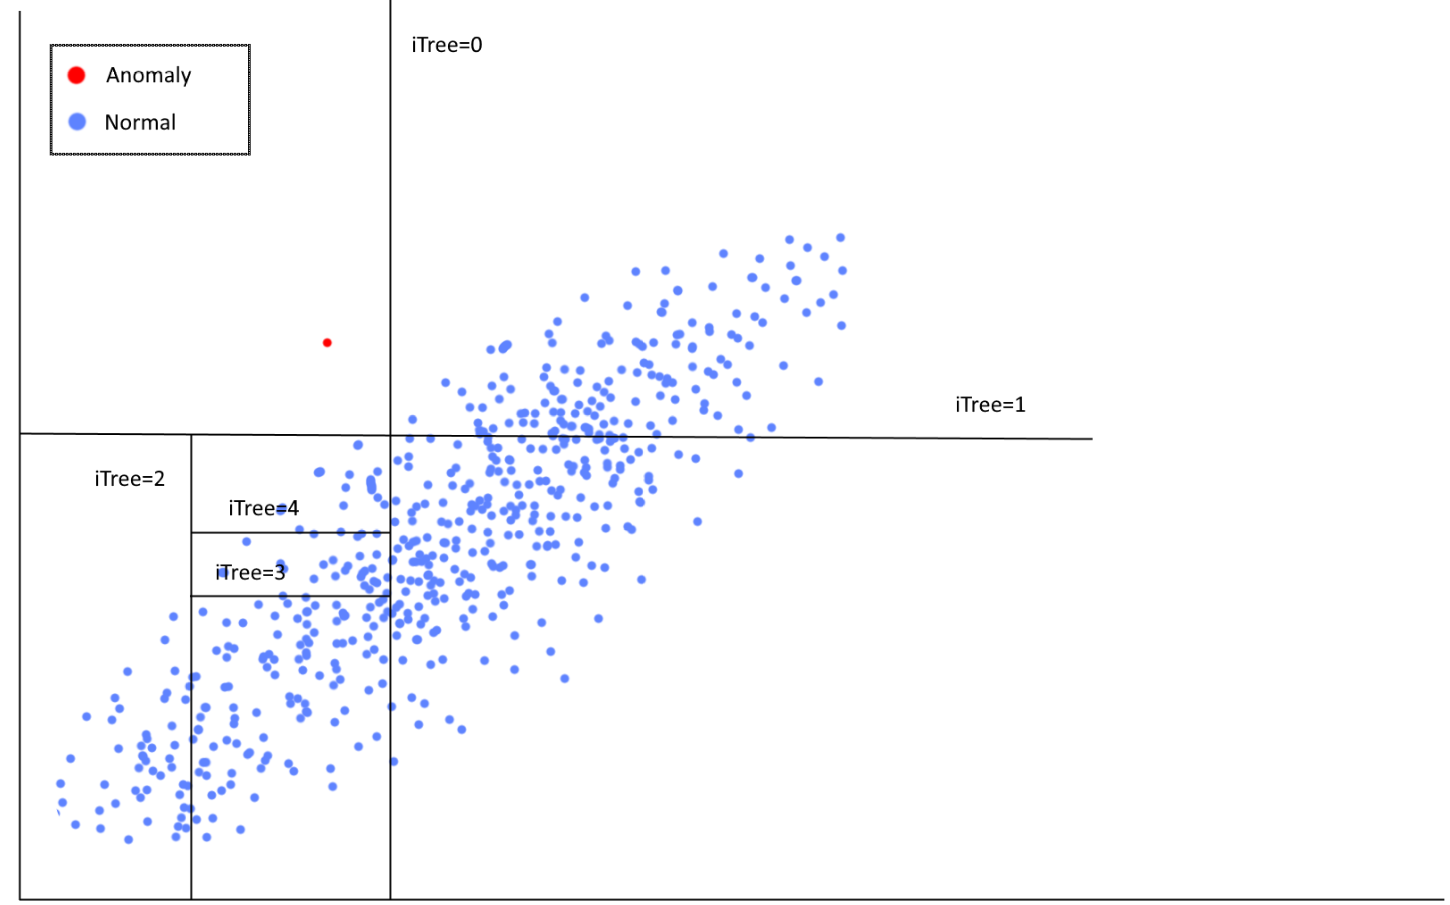
\includegraphics[width=\textwidth]{iTrees.png}
			\caption{Isolation Forest}
			\label{fig:iTrees}
		\end{figure}
		
		O Isolation Forest παρουσιάστηκε από τον Liu \cite{TonyMingZhiHua2008IsolationForest} και είναι μία μέθοδος που χωρίζει τον χώρο πολλαπλές φορές μέχρι να απομονώσει τα σημεία. Είναι μία ensemble μέθοδος που χρησιμοποιεί τα iTrees (τα οποία είναι μία δυαδική διαμέριση του χώρου) για το διαχωρισμό του χώρου. Συνήθως οι ανωμαλίες απομονώνονται σε μόλις λίγα βήματα. Στο Σχ.~\ref{fig:iTrees} βλέπουμε μια ανωμαλία που απομονώθηκε σε μόλις 2 βήματα. Αντίθετα για να απομονωθούν τα φυσιολογικά σημεία απαιτούνται αρκετά βήματα.
		
		Η μέθοδος υλοποιείται σε δύο βήματα: πρώτον δημιουργούμε $n$ iTrees κατά την εκπαίδευση και στο δεύτερο βήμα της αξιολόγησης υπολογίζουμε το σκορ ανωμαλίας.
		
		Για να εφαρμόσουμε τον Isolation Forest στο πλαίσιο τον χρονοσειρών αρχικά θα πρέπει να ορίσουμε ένα παράθυρο και στη συνέχεια να εφαρμόσουμε τον αλγόριθμο στο σύνολο των υπακολουθιών. Το σκορ ανωμαλίας βγαίνει από το μέσο όρο των μηκών των δέντρων, δηλαδή το βάθος του Forest. 
		
		Οι κύριες δυσκολίες αυτής τη μεθόδου είναι τρεις, το μέγεθος του παραθύρου, ο αριθμός των δέντρων και η παράμετρος contamination. Εάν το μέγεθος του παραθύρου είναι μικρό τότε δεν θα υπάρχουν αρκετά δεδομένα ώστε να μπορέσει να φτιαχτεί ένα καλό μοντέλο. Από την άλλη αν είναι μεγάλο, τότε τα παλαιότερα χρονικά δεδομένα θα έχουν το ίδιο βάρος με τα νεότερα. Επιπλέον αν ο αριθμός των δέντρων είναι μεγάλος τότε είναι πιο κοντά στην αναμενόμενη τιμή, όμως, το κύριο πρόβλημα είναι ότι αυξάνεται η υπολογιστική πολυπλοκότητα διότι ο αλγόριθμος τρέχει σε $O(Lw^2)$, όπου $L$ είναι ο αριθμός των δέντρων που κατασκευάζονται και $w$ είναι το μέγεθος του παραθύρου. Τέλος πολλές υλοποιήσεις βασίζονται σε μια παράμετρο που λέγεται contamination, η οποία δείχνει το ποσοστό των ανωμαλιών που περιέχει το σύνολο δεδομένων μας. Η παράμετρος αυτή επηρεάζει το φράγμα για τον εντοπισμό των ανωμαλιών έτσι εάν κάνουμε κακή επιλογή κινδυνεύουμε να πάρουμε αρκετά false positives ή false negatives.
		
		\item \textbf{Άλλες τεχνικές.}
		
		Μία ενδιαφέρουσα τεχνική που πρέπει να αναφερθεί είναι μια παραλλαγή του αλγόριθμου SVM που ονομάζεται \textbf{OC-SVM} \cite{vapnik1964class, ocsvm1999anomalydetection}. Τέλος έχουμε και τον γνωστό αλγόριθμο \\ \textbf{XGBoost} που είναι μια Boosting τεχνική \cite{Chen_2016}.
	\end{itemize}
	
	\section{Μέθοδοι Βαθιάς Μηχανικής Μάθησης}
	Οι μέθοδοι αυτοί μοιάζουν με τις μεθόδους της Μηχανικής Μάθησης διότι δεν θεωρούν ότι τα δεδομένα προέρχονται με κάποιο μηχανισμό από πίσω. Θεωρούν το μηχανισμό σαν μαύρο κουτί και προσπαθούν να κάνουν προβλέψεις εμπειρικά. Σε αυτήν την ενότητα θα δούμε μεθόδους που στηρίζονται στα Νευρωνικά Δίκτυα.
	
	\begin{itemize}
		\item \textbf{Multiple Layer Perceptron.}
		
		Η βασικότερη αρχιτεκτονική των νευρωνικών δικτύων είναι το MLP. Εδώ θα ορίσουμε ένα παράθυρο μήκους $w$. Στη συνέχεια θα πάρουμε τις υπακολουθίες και θα κάνουμε πρόβλεψη με τον εξής τρόπο: για την υπακολουθία $(x_{i-w}, x_{i-w+1}, ... , x_{i})$ μπορούμε να προβλέψουμε την επόμενη τιμή $\hat{y} = f(x_{i+1}) $. Εναλλακτικά μπορούμε να προβλέψουμε μεγαλύτερο διάστημα μήκους $m$, $\hat{y} = f((x_{i+1}, x_{i+2},....,x_{i+m}))$. Το διάστημα μήκος $m$ λέγεται παράθυρο πρόβλεψης.
		
		Για τον εντοπισμός ανωμαλιών θέτουμε ένα φράγμα $\delta$ και για κάθε πρόβλεψη παίρνουμε το λάθος $\epsilon_i = \hat{y_i} - x_i $ το οποίο θα χρησιμοποιηθεί ώς σκορ ανωμαλίας και έχουμε:
		
		\begin{equation*}
			\varphi(x_i) = \begin{cases}
				1 &,\text{ Αν } \epsilon_i\geq\delta\\
				0 &, \text{ Αλλιώς}
			\end{cases}
		\end{equation*}
		
		Ο αλγόριθμος αυτός έχει πολλές παραμέτρους άρα και αρκετές δυσκολίες. Αρχικά έχουμε το βάθος του δικτύου και το πλάτος του, δηλαδή τον αριθμό των κρυμμένων επιπέδων και τον αριθμό των κόμβων σε κάθε επίπεδο αντίστοιχα. Στη συνέχεια θα πρέπει να ορίσουμε το μήκος του παραθύρου και τέλος έχουμε την συνάρτηση βελτιστοποίησης.
		
		\item \textbf{Convolutional Neural Networks}
		Τα convolutional νευρωνικά δίκτυα έχουν γνωρίσει μεγάλη επιτυχία στον τομέα της αναγνώρισης εικόνας, αναγνώρισης αντικειμένων, στην κατηγοριοποίηση κλπ. Ωστόσο μπορούμε να τα χρησιμοποιήσουμε και στον εντοπισμό ανωμαλιών. Σε αντίθεση με τα MLP δίκτυα τα οποία είναι πλήρως συνδεδεμένα (άρα έχουμε και πολλές παραμέτρους) τα convolutional δίκτυα είναι μερικώς συνδεδεμένα κάτι το οποίο τους επιτρέπει να έχουν λιγότερες μεταβλητές να υπολογίσουν, κάνοντάς τα πιο γρήγορα στην εκπαίδευση ενώ ταυτόχρονα τους επιτρέπει να έχουν μεγαλύτερο βάθος. Επιπροσθέτως τα δίκτυα αυτά χρησιμοποιούν μια τεχνική που λέγεται pooling για την αποφυγή της υπερ-εκπαίδευσης (overfitting). Μία άλλη τεχνική που χρησιμοποιείται συχνά ονομάζεται Batch Normalization \cite{SergeyChristian2015BatchNormalization} η οποία είναι μια εναλλακτική για την dropout δηλαδή μειώνει τη σημαντικότητα αρχικοποίησης τιμών. 
		
		Για να εκπαιδευτεί ένα Convolutional Network εφαρμόζεται ένα φίλτρο (ένας πίνακας δηλαδή $n\times k$, το οποίο συνήθως είναι $3\times 3$, $5\times 5$) το οποίο μετατοπίζεται ώστε να σκανάρει όλα τα δεδομένα και να εφαρμοστεί ο τελεστής της συνέλιξης (convolution) Σχ.~\ref{fig:convfilters}.
		
		\begin{figure}[h]
			\centering
			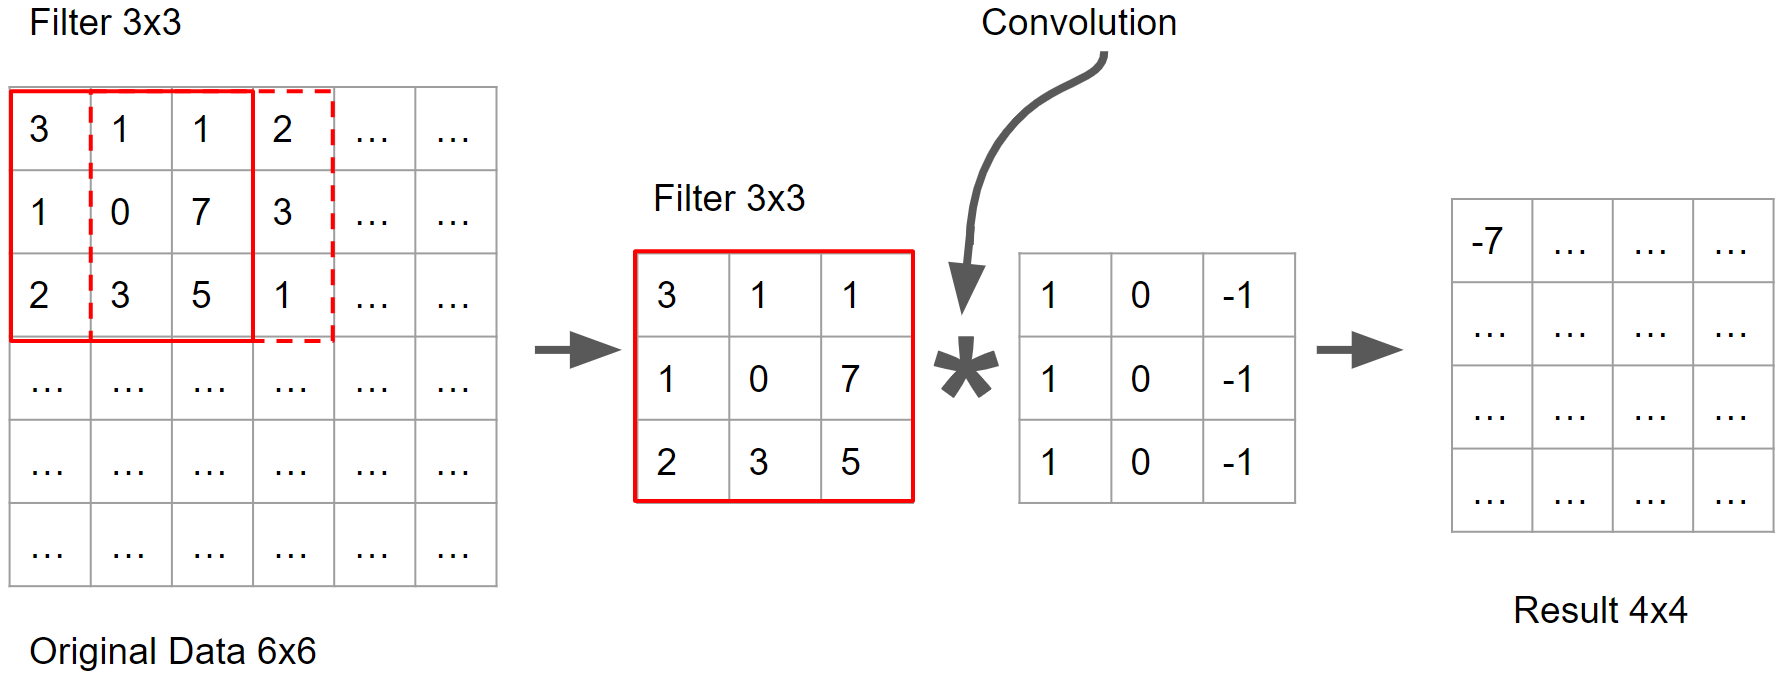
\includegraphics[width=\textwidth/8*7]{convfilters.png}
			\caption{Filter of Convolutonal Layer}
			\label{fig:convfilters}
		\end{figure}
		
		Η χρήση των convolutional στον εντοπισμό ανωμαλιών γίνεται κατά τον ίδιο τρόπο με πριν, δηλαδή ορίζουμε ένα παράθυρο και η εκπαίδευση γίνεται πάνω στις υπακολουθίες. Ο εντοπισμός γίνεται με τον ορισμό ενός φράγματος και τελικά η απόφαση παίρνεται πάνω στα λάθη ανάμεσα στις προβλέψεις και στην πραγματική τιμή, δηλαδή έχουμε ανωμαλία αν $f((x_{i-w}, x_{i-w+1}, ... , x_{i}))-x_{i+1} \geq \delta$
		
		Οι δυσκολίες που αντιμετωπίζει αυτή η μέθοδος είναι κατά κύριο λόγο η αρχιτεκτονική. Εδώ έχουμε μία πολύ μεγάλη δυσκολία διότι η αρχιτεκτονική του δικτύου παίζει μεγάλο ρόλο, δηλαδή έχει σημασία αν θα χρησιμοποιήσουμε dropout, Batch Normalization ή/και max-pooling. Επιπλέον έχει σημασία ο αριθμός και το μέγεθος των πυρήνων που θα χρησιμοποιηθούν σε κάθε convolutional επίπεδο. Πυρήνας ονομάζεται ένα φίλτρο που σαρώνει ένα convolutional επίπεδο το οποίο εξάγει διάφορα χαρακτηριστικά. Τέλος σημαντικός παράγοντας είναι και το βάθος το οποίο θα πρέπει να αποφασιστεί κατά τον ορισμό του δικτύου.
		
		\item \textbf{Residual Neural Network}
		
		\begin{figure}[h]
			\centering
			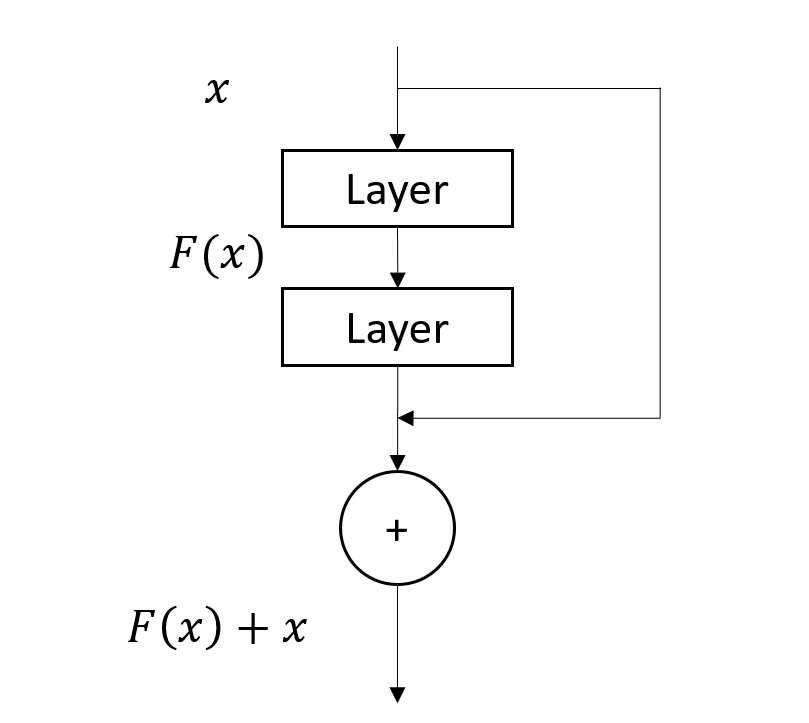
\includegraphics[width=\textwidth/2]{resnetplus.png}
			\caption{Residual Network}
			\label{fig:resnetplus}
		\end{figure}
		
		Τα residual δίκτυα είναι μια επέκταση των Convolutional. Τα δίκτυα αυτά συνδυάζουν ένα αποτέλεσμα από τα προηγούμενα επίπεδα με το αποτέλεσμα ενός μεταγενέστερου επιπέδου Σχ.~\ref{fig:iTrees} το block αυτό ονομάζεται residual block \cite{HeZhangRen2015Residual}. Για να ορίσουμε ένα residual block θεωρούμε ένα $x$ ώς η είσοδος του, και $\varphi$ ένα convolutional block, το οποίο αποτελείται από convolutional επίπεδα, max-pooling, batch normalization κλπ. Η έξοδος ενός residual block είναι $y=x+\varphi(x)$. Συνήθως συμπεριλαμβάνεται και μία συνάρτηση ενεργοποίησης $\varPsi$ και τελικά έχουμε $y=\varPsi(x+\varphi(x))$.
		
		Τα residuals δίκτυα χρησιμοποιούνται για να λύσουν το πρόβλημα της "εξαφάνισης της παραγώγου" που προκύπτει από τα Convolutional δίκτυα λόγω του βάθους τους. Στην ουσία το πρόβλημα αυτό αναφέρεται σε παραγώγους οι οποίες είναι τόσο μικρές που στην ουσία μηδενίζονται (εξαφανίζονται).
		
		\item \textbf{LSTM - Long Short Term Memory Network.}
		
		Ένα δίκτυο γνωστό για την εφαρμογή του σε σειριακά (ακολουθιακά) δεδομένα είναι το δίκτυο LSTM το οποίο ανήκει στην οικογένεια των Recurrent Νευρωνικών Δικτύων. Σε αντίθεση με τα προηγούμενα όπου τα δεδομένα είχαν μια συνεχή πορεία προς τα εμπρός, ένα Recurrent δίκτυο διαθέτει μία σύνδεση με τα δεδομένα που ήδη έχουν περάσει, κάτι το οποίο του επιτρέπει να αντλεί πληροφορία σύμφωνα με άλλα δεδομένα και να συνδυάζει τη γνώση. Επίσημα λοιπόν η έξοδος που παράγεται είναι η εξής:
		
		$$ y_i = h({x_i}^T \cdot {w_x} + {y_{i-1}}^T\cdot {w_y} + b)$$
		
		όπου $h$ είναι η συνάρτηση ενεργοποίησης, $x_i$ είναι ένα στοιχείο από το σύνολο των δεδομένων, $y_{i-1}$ είναι μία "προηγούμενη" προβλεπόμενη τιμή, $w_x, w_y$ είναι τα βάρη και $b$ μία σταθερά.
		
		\begin{figure}[h]
			\centering
			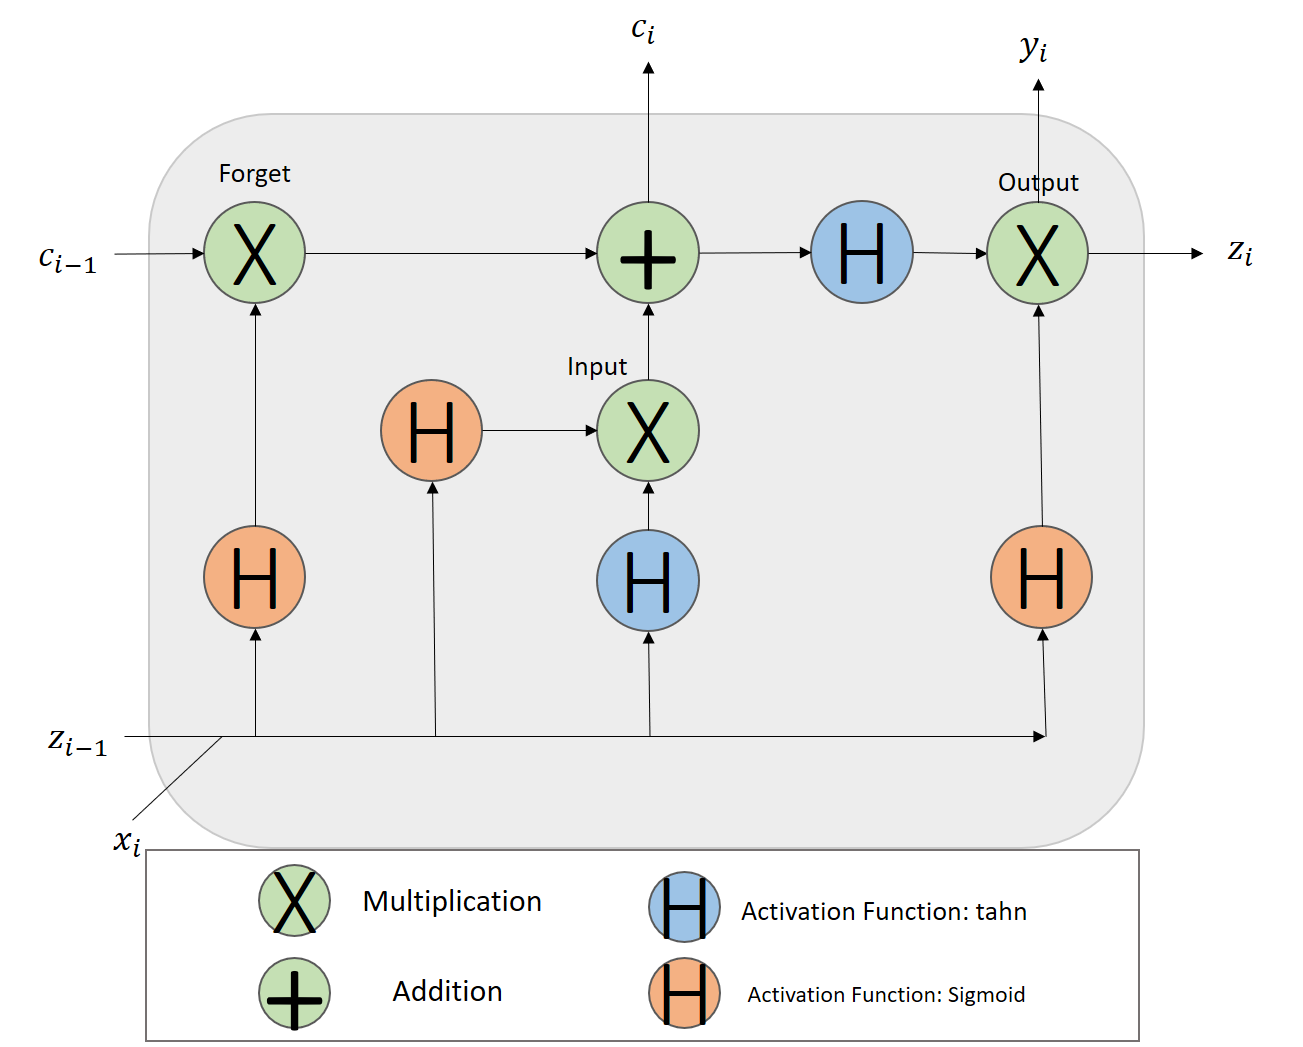
\includegraphics[width=\textwidth]{lstmarchitecture2.png}
			\caption{LSTM}
			\label{fig:lstmarchitecture}
		\end{figure}
		
		Ένα δίκτυο LSTM είναι λοιπόν μια παραλλαγή ενός τέτοιου δικτύου \cite{LSTM1997HochreiterSchmidhuber} στην οποία περιλαμβάνονται δύο διανύσματα $c_i$ και $z_i$. Η $z_i$ προστίθεται με το $x_i$ και καλείται short term ενώ η $c_i$ πολλαπλασιάζεται με το $x_i$ και καλείται long term. Επιπλέον υπάρχουν 3 "πύλες" που ρυθμίζουν την πληροφορία που θα πεταχτεί (forget πύλη), την πληροφορία που θα περάσει (input πύλη) και την πληροφορία που θα αποτελέσει την έξοδο (output πύλη). Αυτός ο σχεδιασμός έχει ώς αποτέλεσμα να αποθηκεύεται σημαντική πληροφορία κατά την πρόσθεση ώστε να χρησιμοποιηθεί πιο μετά (long term) και με τη χρήση του πολλαπλασιασμού (κατά σημείο) επιτυγχάνεται η διαγραφή πληροφορίας που μας είναι άχρηστη σύμφωνα με το μοντέλο από τον long term όρο. Τέλος η πύλη εξόδου αποφασίζει ποιο κομμάτι του long-term όρου θα είναι η έξοδος Σχ.~\ref{fig:lstmarchitecture}.
		
		Τα βήματα που εκτελεί το LSTM είναι τα εξής:
		
		\begin{enumerate}
			\item Καταρχήν θα μεταφερθούμε στην forget πύλη όπου θα αποφασιστεί τι πληροφορία θα πεταχτεί. Παίρνει την είσοδο $x_i$ και την προηγούμενη έξοδο $z_{i-1}$, και με την συνάρτηση ενεργοποίησης Sigmoid (έστω $h_s$) έχουμε $f_i = h_s(W_f\cdot [ z_{i-1, x_i}] + b_f)$. Σαν τελευταίο βήμα όταν πάμε στην πύλη forget πολλαπλασιάζουμε με την παλιά κατάσταση και έχουμε $F_i = f_i \cdot C_{i-1}$
			\item Στη συνέχεια αποφασίζεται τι πληροφορία θα κρατήσει (input πύλη). Αρχικά εφαρμόζεται μία συνάρτηση ενεργοποίησης sigmoid στην είσοδο $x_i$ και στην προηγούμενη έξοδο $z_{i-1}$ η οποία θα αποφασίσει ποιες τιμές πρέπει να ανανεωθούν $u_i = h_s(W_u \cdot [z_{i-1}, x_i] + b_u)$. Και δεύτερον θα εφαρμοστεί μία συνάρτηση ενεργοποίησης tanh (έστω $h_\text{tanh}$),  $\hat{C_i} = h_\text{tanh}(W_C \cdot [z_{i-1}, x_i] + b_C)$ για την ανανέωση. Τελικά θα πάρουμε μετά την εφαρμογή της πύλης input $I_i = u_i \cdot \hat{C_i}$
			\item Στην συνέχεια συνδυάζουμε τα δύο προηγούμενα βήματα δηλαδή εφαρμόζουμε μία πρόσθεση και έχουμε $ C_i = F_i + I_i$
			\item Εφόσον έχουν γίνει τα προηγούμενα βήματα τώρα είναι η στιγμή που θα αποφασιστεί η έξοδος. Αρχικά περνάμε το προηγούμενο αποτέλεσμα από τη συνάρτηση ενεργοποίησης tanh ώστε να περιορίσουμε τις τιμές στο διάστημα -1, 1 παίρνοντας $r_i = h_\text{tanh}(C_i)$ και μετά θα περάσουμε την είσοδο $x_i$ και την προηγούμενη έξοδο από την συνάρτηση ενεργοποίησης sigmoid για να πάρουμε $o_i = h_s(W_o \cdot [z_{i-1}, x_i] + b_o)$. Μετά τον πολλαπλασιασμό θα πάρουμε την έξοδο από την πύλη output $O_i = o_i \cdot r_i$
			\item κατά τη διάρκεια της διαδικασία αυτής αποθηκεύονται οι τιμές των $C_i$, $O_i=z_i$ για μελλοντική χρήση
		\end{enumerate}
		
		\item \textbf{Autoencoder.}
		
		Η μέθοδος autoencoder υλοποιείται σε δύο βήματα. Στο πρώτο βήμα το μοντέλο κωδικοποιεί την είσοδο και στο δεύτερο βήμα αποκωδικοποιεί την είσοδο Σχ.~\ref{fig:autoencoder}. Η κύρια ιδέα πίσω από αυτόν τον αλγόριθμο είναι ότι αν προβάλουμε τα σημεία σε έναν χώρο λιγότερων διαστάσεων τα φυσιολογικά δεδομένα θα διαφέρουν σημαντικά από τις ανωμαλίες. Οπότε αν κάνουμε την αντίστροφη διαδικασία, τα σημεία που έχουν σημαντικές διαφορές σε σχέση με την αρχική τους κατάσταση θα είναι ανωμαλίες. Αυτή η ιδέα κάνει τον autoencoder πολύ καλή επιλογή για την ανίχνευση ανωμαλιών.
		
		\begin{figure}[h]
			\centering
			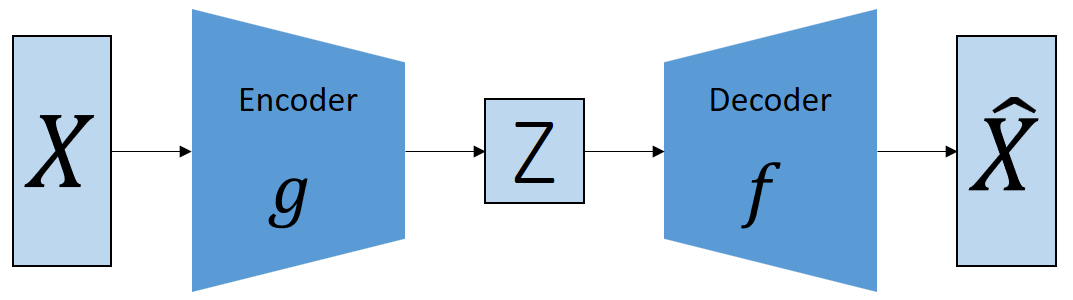
\includegraphics[width=\textwidth]{autoencoder.png}
			\caption{Autoencoder}
			\label{fig:autoencoder}
		\end{figure}
		
		Τέτοιου τύπου δίκτυα ανήκουν στην οικογένεια των δικτύων εμπρόσθιας τροφοδότησης ή αλλιώς feed-forward (όπως ήταν και ο αλγόριθμος MLP που είδαμε νωρίτερα) σε αντίθεση με τα LSTM. Το πρώτο βήμα της διαδικασίας ονομάζεται κωδικοποιητής (Encoder) ενώ το δεύτερο αποκωδικοποιητής (Decoder). Επίσημα έχουμε:
		
		Έστω $\mathcal{X}$ το σύνολο δεδομένων, $f$ η συνάρτηση decoder και $g$ η συνάρτηση encoder, έχουμε:
		
		$$\hat{X} = f(g(X))$$
		
		Η συνάρτηση βελτιστοποίησης θα προσπαθήσει να μειώσει τη διαφορά ανάμεσα στο $\hat{X}$ και $X$, δηλαδή:
		
		$$\min_{w_f, w_g} \lvert \lvert X - \hat{X} \rvert \rvert_2  = \min_{w_f, w_g} \lvert \lvert X - f(g(X)) \rvert \rvert_2$$
		
		Τελικά από κάθε $x_i$ παίρνουμε ένα $\hat{x_i}$ και έχουμε το λάθος $\epsilon = \lvert x_i - \hat{x_i} \rvert$ το οποίο το χρησιμοποιούμε σαν σκορ ανωμαλίας. Ορίζοντας ένα φράγμα $\delta$ μπορούμε να αποφασίσουμε τι είναι ανωμαλία και τι όχι.
		
		Συχνά τα autoencoder συνδυάζονται με άλλα δίκτυα, για παράδειγμα CNN δίκτυα ή LSTM. Με αυτή την σύνθεση το ρόλο των encoder/decoder παίρνουν αυτά τα δίκτυα και το αποτέλεσμα είναι να πάρουμε τα πλεονεκτήματα και των δύο τεχνικών. Η διαδικασία είναι η εξής: αρχικά τα δεδομένα περνάνε από το δίκτυο (πρώτο βήμα Encoding) ώστε να μειωθούν οι διαστάσεις και στη συνέχεια στο ίδιο δίκτυο με την αντίστροφη αρχιτεκτονική (δεύτερο βήμα Decoding) ώστε να ξαναπάρουμε ένα στοιχείου του αρχικού χώρου. Οι ανωμαλίες εντοπίζονται όπως είπαμε πριν.
		
		\item \textbf{Variational Autoencoder και LSTM-VAE}
		
		\begin{figure}[h]
			\centering
			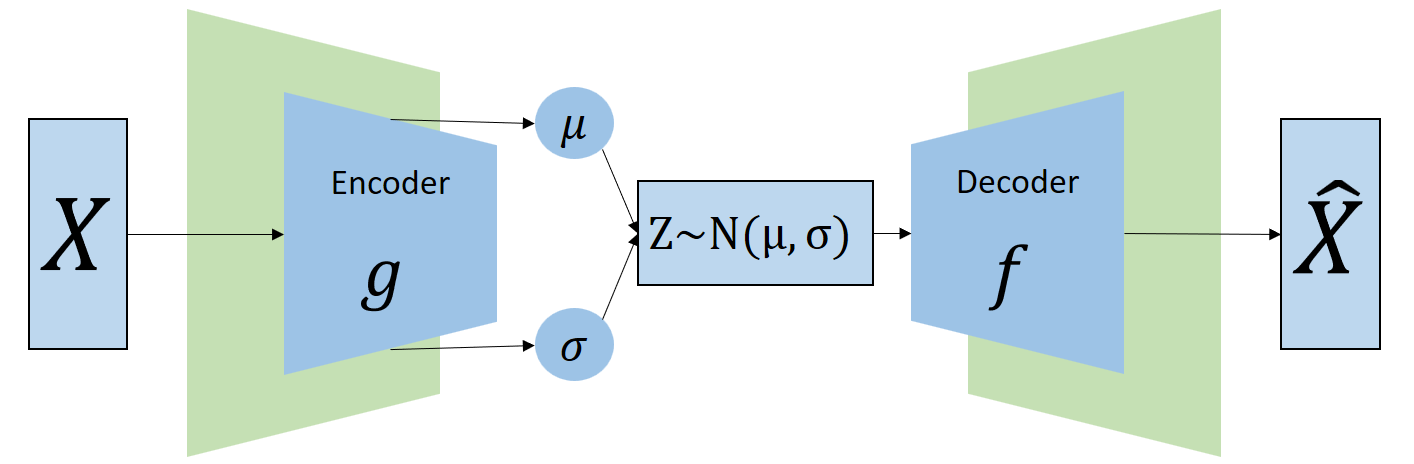
\includegraphics[width=\textwidth/8*7]{lstmvae.png}
			\caption{LSTM-VAE}
			\label{fig:lstmvae}
		\end{figure}
		
		Παραλλαγή του autoencoder είναι ο Variational autoencoder (ή Auto-Encoding Variational Bayes \cite{Kingma2013WellingVAE}) όπου επιλέγεται δειγματοληπτικά ένα Z από μία κανονική κατανομή, ενώ ο encoder και ο decoder είναι η posterior $q(z;x)$ και η prior $p(\hat{x};z)$.
		
		To δίκτυο LSTM-VAE συνδυάζει έναν Variational Autoencoder με ένα LSTM Σχ.~\ref{fig:lstmvae} το οποίο στην πραγματικότητα είναι μια παραλλαγή του LSTM-AΕ.
		
		
		
		
		\item \textbf{Άλλες τεχνικές.}
		
		Επιπλέον πριν κλείσουμε αυτήν την ενότητα θα πρέπει να κάνουμε μια αναφορά σε δίκτυα που αξίζει να αναφερθούν όπως το WaveNet \cite{Oord2016WaveNet} και μια παραλλαγή του LSTM το GRU \cite{ChoMerrienboer2014GRURNN}. Στην περίπτωση του WaveNet η χρονοσειρά εισάγεται όπως ακριβώς και σε ένα convolutional δίκτυο, ορίζοντας ένα παράθυρο το οποίο ορίζει υπακολουθίες οι οποίες με τη σειρά τους δίνονται στο μοντέλο. Η η κυριότερη διαφορά του WaveNet με το convolutional είναι ότι το WaveNet χρησιμοποιεί διαστελλόμενα φίλτρα Σχ.~\ref{fig:dilationfilters}. 
		
		\begin{figure}[h]
			\begin{subfigure}[b]{0.4\textwidth}
				\centering
				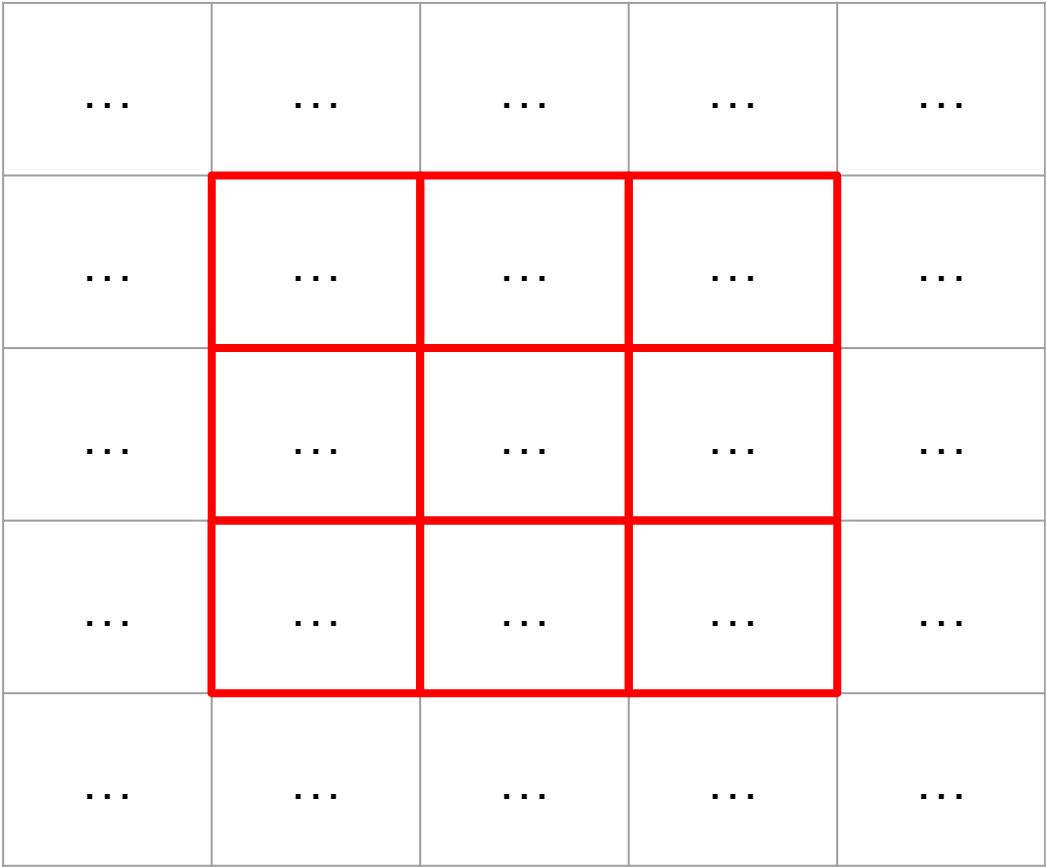
\includegraphics[width=\textwidth]{dilationfilters_withoutdilation.png}
				\caption{Without dilation (Χωρίς διαστολή)}
				\label{fig:dilationfilters_withoutdilation}
			\end{subfigure}
			\hfill
			\begin{subfigure}[b]{0.4\textwidth}
				\centering
				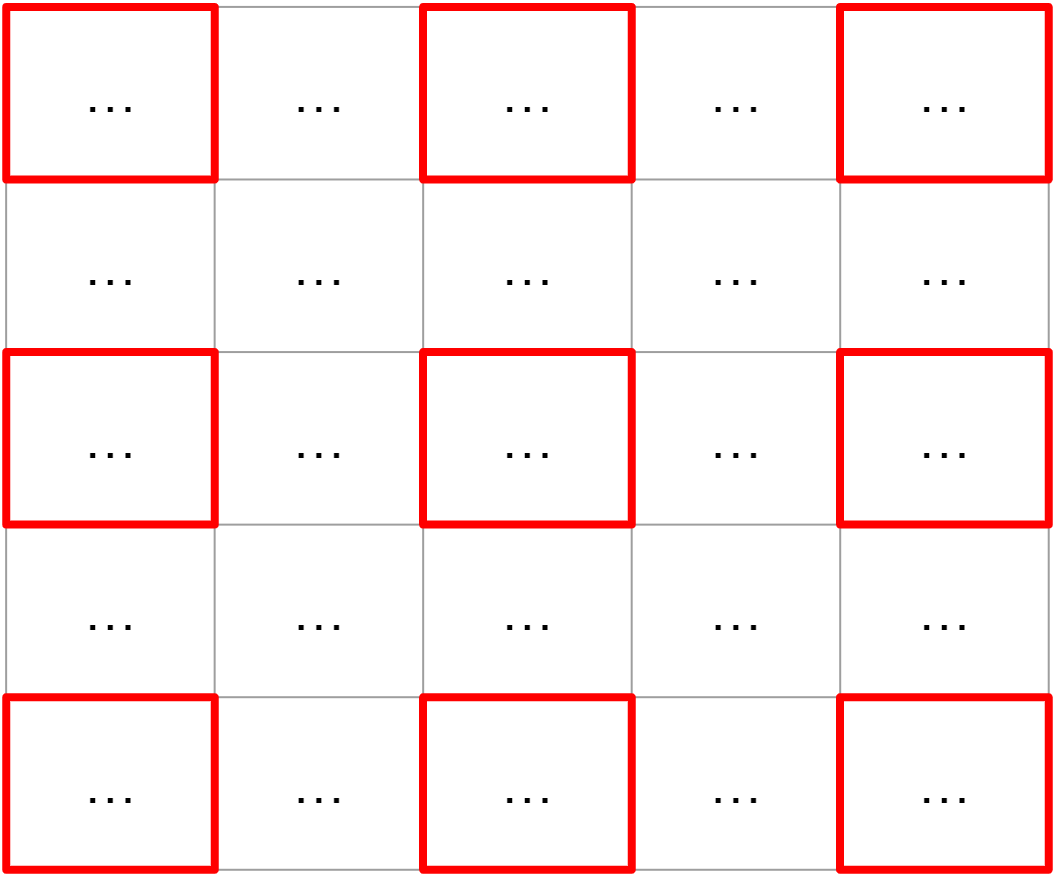
\includegraphics[width=\textwidth]{dilationfilters_withdilation.png}
				\caption{With dilation (Με διαστολή)}
				\label{fig:dilationfilters_withdilation}
			\end{subfigure}
			\caption{no dilation vs dilation}
			\label{fig:dilationfilters}
		\end{figure}
		
		Από την άλλη το GRU είναι μία παραλλαγή του LSTM, οι χρονοσειρές εισάγονται κατά τον ίδιο τρόπο με το LSTM ορίζοντας ένα παράθυρο μήκους $w$. Η ομοιότητα με το LSTM είναι μεγάλη και στη βιβλιογραφία φαίνεται να έχουν τις ίδιες επιδόσεις. Η μεγαλύτερη διαφορά είναι ότι το GRU έχει πιο απλή δομή Σχ.~\ref{fig:lstmgrucomparison}. Ως εκ τούτου έχει λιγότερες μεταβλητές και άρα εκπαιδεύεται σε λιγότερο χρόνο.
		
		\begin{figure}[h]
			\centering
			\begin{subfigure}[b]{0.8\textwidth}
				\centering
				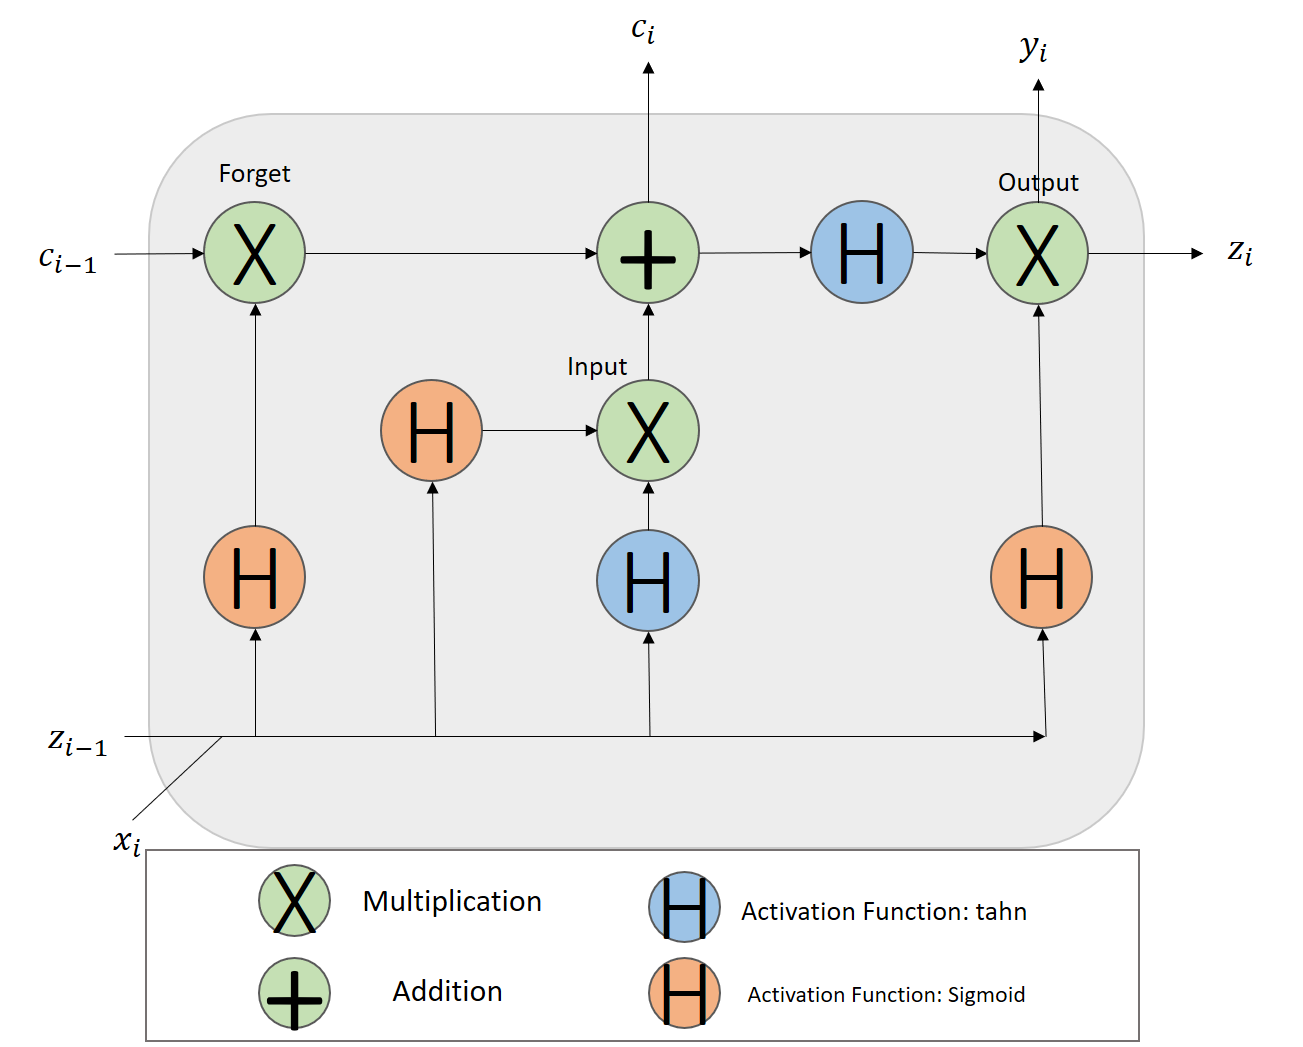
\includegraphics[width=\textwidth]{lstmarchitecture2.png}
				\caption{LSTM}
				\label{fig:lstmarchitecturecell}
			\end{subfigure}
			\hfill
			\begin{subfigure}[b]{0.8\textwidth}
				\centering
				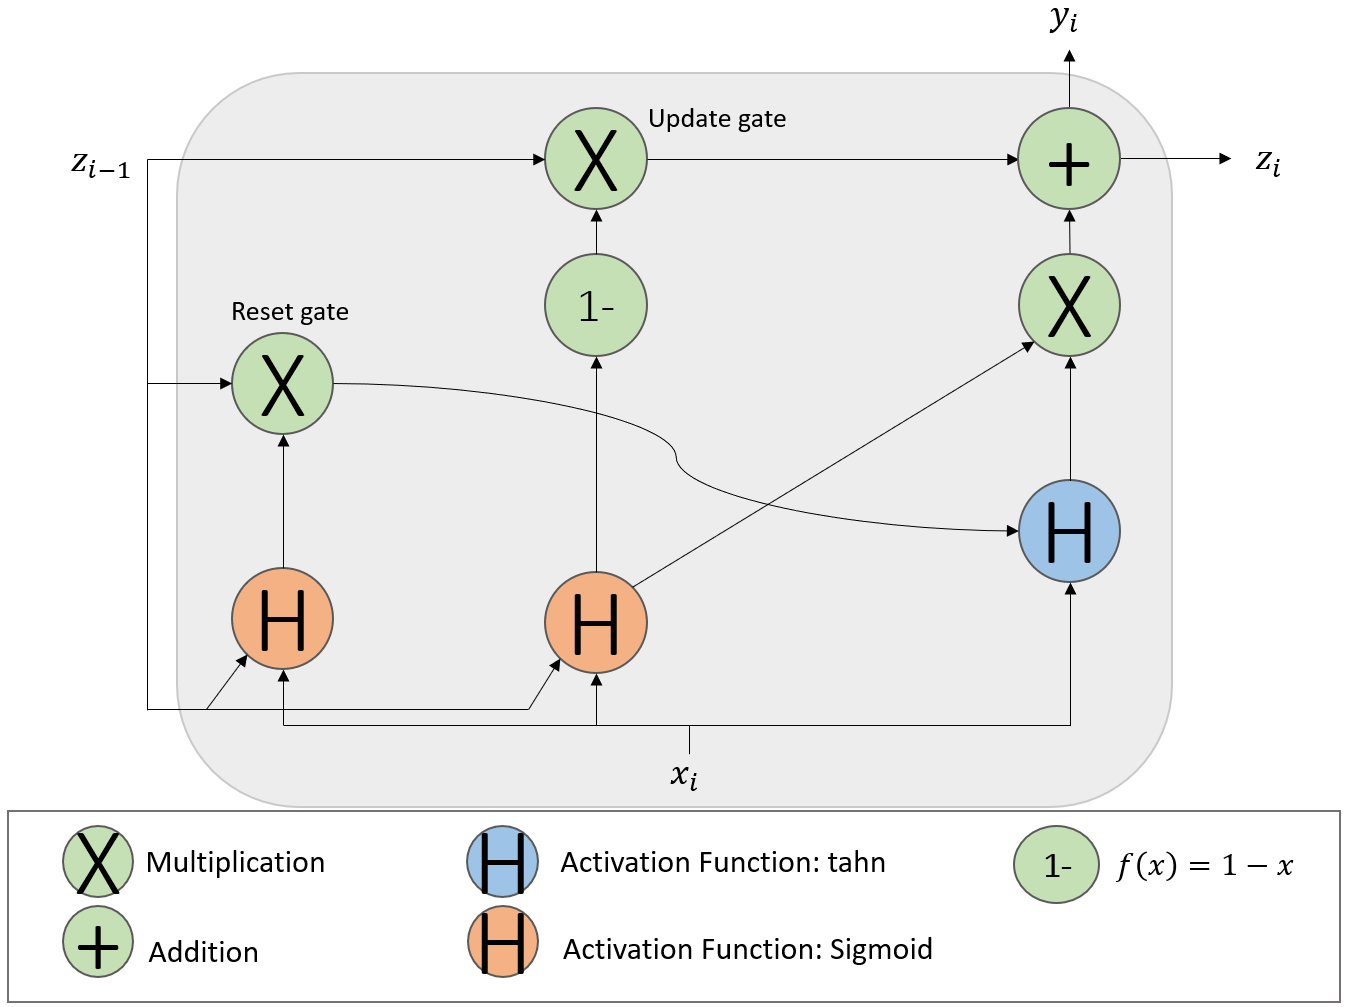
\includegraphics[width=\textwidth]{gruarchitecture2.png}
				\caption{GRU}
				\label{fig:gruarchitecturecell}
			\end{subfigure}
			\caption{LSTM cell vs GRU cell}
			\label{fig:lstmgrucomparison}
		\end{figure}
		
	\end{itemize}
	
	
	\chapter{Ανίχνευση εξαιρέσεων σε δεδομένα χρονοσειρών με χρήση ensemble τεχνικών}
	\section{Ensemble}
	Στο κεφάλαιο αυτό θα δούμε κάποιες τεχνικές ensemble οι οποίες θα συγκριθούν με τους βασικούς αλγόριθμους στους οποίους στηρίζονται. Ensemble ονομάζονται οι μέθοδοι machine learning που βασίζονται σε άλλα μοντέλα. Στην ουσία συγκεντρώνουν τα αποτελέσματα άλλων μοντέλων και τα συνδυάζουν σε ένα τελικό αποτέλεσμα. Η ομάδα των μοντέλων και ο συνδυασμός τους ονομάζεται Ensemble. Τα ensemble μοντέλα έχουν χρησιμοποιηθεί αρκετά σε διάφορους τύπους προβλημάτων, όπως στην κατηγοριοποίηση ή στην πρόβλεψη τιμών. Γνωστοί αλγόριθμοι όπως οι Random Forest και Majority Voting έχουν μεγάλη επιτυχία σε τέτοιου είδους προβλήματα. Αλλά και πιο σύνθετοι αλγόριθμοι όπως το Bagging, το boosting και το Stacking έχουν χρησιμοποιηθεί πολύ. Η μέθοδος Bagging αποτελείται από δύο βήματα. Στο πρώτο βήμα έχουμε κάποια αρχικά μοντέλα και επιλέγουμε μόνο μερικά από τα δεδομένα για κάθε ένα μοντέλο ώστε να εκπαιδευτεί σε περιορισμένο αριθμό παρατηρήσεων. Αυτό έχει ως αποτέλεσμα το κάθε μοντέλο να βρίσκει διαφορετικά μοτίβα στο σύνολο των δεδομένων. Στο δεύτερο βήμα συγκεντρώνουμε τα αποτελέσματα και καταλήγουμε σε μία πρόβλεψη η οποία προκύπτει από το συνδυασμό των επιμέρους προβλέψεων. Στη μέθοδο boosting εκπαιδεύουμε τα μοντέλα κατά σειρά το ένα μετά το άλλο, δίνοντας στο ένα μοντέλο την έξοδο του προηγούμενου. Έτσι ένα μοντέλο εκπαιδεύεται από τα λάθη του προηγούμενού του με αποτέλεσμα όσο η διαδικασία προχωράει τα μοντέλα που βρίσκονται προς το τέλος να γίνονται πιο ισχυρά. Στην τεχνική stacking, σε αντίθεση με το boosting, όλα τα μοντέλα εκπαιδεύονται παράλληλα, ενώ η διαφορά με την τεχνική bagging είναι ότι η εκπαίδευση όλων των μοντέλων γίνεται σε όλα τα δεδομένα από το σύνολο δεδομένων εκπαίδευσης. Στο τελικό στάδιο ενός stacking βρίσκεται ένα μοντέλο το οποίο θα εκπαιδευτεί ώστε να συνδυάζει σωστά τα αποτελέσματα των υπόλοιπων μοντέλων. Το τελικό μοντέλο ονομάζεται μετα-μοντέλο. 
	
	Παρόλο που οι ensemble τεχνικές είναι διαδεδομένες, στο χώρο της ανίχνευσης ανωμαλιών σε χρονοσειρές πολλών μεταβλητών δεν έχουν μελετηθεί τόσο πολύ. Σε αυτή τη διπλωματική δίνουμε ensemble τεχνικές που έχουν χρησιμοποιηθεί για άλλου είδους προβλήματα ενώ ταυτόχρονα συγκρίνουμε τα αποτελέσματα με τους βασικούς αλγόριθμους που χρησιμοποιήθηκαν για να συνθέσουν τα ensemble. Επίσης θα δώσουμε και μία υλοποίηση η οποία δεν βρέθηκε στην βιβλιογραφία της ανίχνευσης ανωμαλιών, τουλάχιστον όσον αφορά την προσωπική μας αναζήτηση. Τελικά θα χρησιμοποιήσουμε τις παραπάνω τεχνικές όπως το bagging και το stacking. Αρχικά θα δημιουργήσουμε μοντέλα από την τεχνική bagging δίνοντας και στη συνέχεια θα δώσουμε τις εξόδους τους σε ένα μετα-μοντέλο σύμφωνα με την τεχνική του stacking. 
	
	Στις παρακάτω τεχνικές που θα δούμε έχουμε χρησιμοποιήσει παντού τα ίδια μοντέλα τα οποία είναι: Autoencoder, LSTM, Autoencoder με LSTM (LSTM-AE), Convοlutional Autoencoder (CONV-AE) και ένα LSTM-VAE.
	\section{Δεδομένα}
	
	Tα dataset που έχουν χρησιμοποιηθεί είναι από το SKAB (Skoltech Anomaly Benchmark) \cite{skabdataset}. Τα dataset έχουν παραχθεί από μία συσκευή η οποία περιλαμβάνει:
	
	\begin{itemize}
		\item Ένα σύστημα κυκλοφορίας νερού.
		\item Ένα σύστημα ελέγχου της κυκλοφορίας νερού.
		\item Ένα σύστημα για την παρακολούθηση της κατάστασης του νερού στο σύστημα κυκλοφορίας.
		\item Μία τεχνολογία (TSN) για την καταγραφή του χρόνου.
		\item Τέλος ένα σύστημα για την αποθήκευση δεδομένων.
	\end{itemize}
	Επίσης η συσκευή αυτή διαθέτη βαλβίδες και μηχανισμούς ώστε να δημιουργεί μη-φυσιολογική λειτουργία αλλά και αισθητήρες.
	
	Τα δεδομένα είναι χρονοσειρές πολλών μεταβλητών. Κάθε γραμμή μέσα στα dataset συμβολίζει μία καταγραφή μίας δεδομένης χρονικής στιγμής η οποία αποτελείται από 8 μεταβλητές, τη χρονική στιγμή που έγινε η παρατήρηση και την ένδειξη αν είναι ανωμαλία ή όχι:
	
	\begin{itemize}
		\item datetime - Είναι η χρονική στιγμή που καταγράφεται η παρατήρηση.
		\item Accelerometer1RMS - Επιτάχυνση (μονάδα g)
		\item Accelerometer2RMS - Επιτάχυνση (μονάδα g)
		\item Current - Δείχνει το ρεύμα (μονάδα Ampere)
		\item Pressure - Πίεση (μονάδα Bar)
		\item Temperature - Θερμοκρασία (Βαθμοί Κελσίου)
		\item Thermocouple - Θερμοκρασία (Βαθμοί Κελσίου)
		\item Voltage - Τα βολτ του μηχανήματος (μονάδα Volt)
		\item RateRMS - Ρυθμός κυκλοφορίας ροής του ρευστού μέσα στο βρόγχο (Μονάδα Λίτρα/Λεπτό)
		\item anomaly - Δείχνει αν το σημείο είναι ανωμαλία (0 ή 1)
	\end{itemize}
	
	Τα δεδομένα προσομοιώνουν διάφορες καταστάσεις (κάθε σύνολο δεδομένων περιγράφει διαφορετική κατάσταση και συνολικά έχουμε επιλέξει 31 σύνολα δεδομένων) όπως για παράδειγμα Προσομοίωση διαρροής υγρού και προσθήκη, Απότομη συμπεριφορά ανισορροπίας, Απότομη αύξηση/μείωση υγρού, Αργή αύξηση υγρού, Αύξηση υγρού υψηλής θερμοκρασίας και άλλα. Ανάλογα με την περίπτωση έχει φτιαχτεί διαφορετικό σύνολο δεδομένων όπου αρχικά το σύστημα δουλεύει σε φυσιολογικές συνθήκες και στη συνέχεια γίνεται η προσομοίωση ενός σεναρίου όπου παρατηρούμε τις ανωμαλίες.
	
	Το SKAB λοιπόν είναι μία συλλογή από δεδομένα τα οποία μπορούν να χρησιμοποιηθούν για την αξιολόγηση τεχνικών και μοντέλων στο πλαίσιο της έρευνας στην Ανίχνευση Ανωμαλιών σε χρονοσειρές πολλών μεταβλητών. Οι συγγραφείς στο \cite{skabdataset} έχουν πειραματιστεί με αρκετά από τα μοντέλα που έχουμε ήδη περιγράψει όπως Convolutional Autoencoder, LSTM, LSTM Variational Autoencoder, Isolation forest και άλλα. Τα αποτελέσματα που πέτυχαν δείχνουν ότι πετυχαίνουν 0.79 F1-Score με το Convolutional Autoencoder στην πρώτη θέση ενώ στην τελευταία θέση βρίσκεται το Isolation Forest με 0.4 F1-Score, Πίνακας~\ref{tab:skabresults}. Στο \cite{elhalwagy2022hybridization} προτείνεται μία νέα αρχιτεκτονική Νευρωνικού Δικτύου από την οποία προκύπτει ένα υβριδικό Δίκτυο που προέρχεται από τα δίκτυα Capsule και LSTM. Οι συγγραφείς χρησιμοποιούν τα datasets του SKAB για να αξιολογήσουν την αρχιτεκτονική τους. Και εδώ παρατηρούμε τα αποτελέσματα να κυμαίνονται στα ίδια επίπεδα με ένα LSTMCaps στην πρώτη θέση με 0.74 F1-Score ενώ το Isolation Forest βρίσκεται στην τελευταία θέση με 0.4 F1-Score Πίνακας~\ref{tab:capsuleandlstm}. Τέλος στο \cite{pranavan2022contrastive} προτείνεται ένα μοντέλο που ονομάζεται TRL-CPC το οποίο μαθαίνει να αναπαριστά τη χρονοσειρά μέσω του Contrastive Learning. Contrastive Learning λέγεται η εκπαίδευση ενός μοντέλου όπου τα δείγματα συγκρίνονται μεταξύ τους και το μοντέλο μαθαίνει να βρίσκει τις ομοιότητες των χαρακτηριστικών των δειγμάτων που ανήκουν στην ίδια κλάση. Οι συγγραφείς καταφέρνουν να πετύχουν ένα  0.70 F1-Score με το TRL-CPC  στο σύνολο δεδομένων του SKAB.  
	
	\begin{table}[H]
		\begin{subtable}[h]{0.31\textwidth}
			\centering
			\resizebox{\textwidth}{!}{
				\begin{tabular}{|c|c|}
					\hline
					Model Title & F1 Score \\
					\hline
					Conv-AE & 0.79 \\
					\hline
					MSET & 0.73 \\
					\hline
					LSTM-AE & 0.68 \\
					\hline
					T-squared+Q (PCA) & 0.67 \\
					\hline
					LSTM & 0.64 \\
					\hline
					MSCRED & 0.64 \\
					\hline
					LSTM-VAE & 0.56 \\
					\hline
					T-squared & 0.56 \\
					\hline
					Autoencoder & 0.45 \\
					\hline
					Isolation forest & 0.4 \\
					\hline
				\end{tabular}
			}
			\caption{SKAB Results}
			\label{tab:skabresults}
		\end{subtable}
		\hfill
		\begin{subtable}[h]{0.31\textwidth}
			\centering
			\resizebox{\textwidth}{!}{
				\begin{tabular}{|c|c|}
					\hline
					Model Title & F1 Score \\
					\hline
					LSTMCaps & 0.74 \\
					\hline
					MSET & 0.73 \\
					\hline
					LSTMCapsV2 & 0.71 \\
					\hline
					MSCRED & 0.7 \\
					\hline
					LSTM & 0.67 \\
					\hline
					Conv-AE & 0.66 \\
					\hline
					LSTM-AE & 0.65 \\
					\hline
					LSTM-VAE & 0.56 \\
					\hline
					Autoencoder & 0.45 \\
					\hline
					Isolation forest & 0.4 \\
					\hline
				\end{tabular}
			}
			\caption{Hybridization of Capsule and LSTM Networks}
			\label{tab:capsuleandlstm}
		\end{subtable}
		\caption{Αποτελέσματα από άλλες ερευνητικές εργασίες}
		\label{tab:otherresearchresults}
	\end{table}
	
	\section{Majority Voting}
	Η λογική του Majoriy Voting στηρίζεται στο εξής: Αν κάνουμε μια ερώτηση σε 1000 ανθρώπους τότε κατά πάσα πιθανότητα η πλειοψηφία να βρει τη σωστή απάντηση. Αυτό ονομάζεται "η σοφία της πλειοψηφίας". Στα μαθηματικά αυτό δείχνεται με τη βοήθεια της διωνυμικής κατανομής: Έστω $X_i$ ανεξάρτητες και ισόνομες τυχαίες μεταβλητές με $ X_i \sim bernoulli(p), \quad i=1,2,....,1000$ όπου η πιθανότητα σωστής απάντησης είναι $ p=51\% $. Οι $X_i$ αναλογούν στους ανθρώπους και η πιθανότητα 51\% αναλογεί στην ικανότητά τους να απαντάνε σωστά. Δηλαδή είναι ελάχιστα καλύτεροι από το να απαντούσαν στην τύχη γυρίζοντας ένα νόμισμα. Τότε η πιθανότητα πάνω από τους μισούς να απαντήσουν σωστά είναι $P(X\geq501) = 1-P(X\leq500)$. Από τη διωνυμική κατανομή ξέρουμε ότι $P(X\leq500) = \mathlarger{\sum\limits_{n=0}^{499}} \mathlarger{\binom{\mathlarger{1000}}{\mathlarger{n}}} (\frac{51}{100})^n(1-\frac{51}{100})^{1000-n} \approx 25\%$. Οπότε έχουμε ότι $P(X\geq 501)\approx75\%$. Το οποίο σημαίνει ότι έχουμε 75\% πιθανότητα περισσότεροι από 500 άτομα να απαντήσουν σωστά. Όσο αυξάνουμε τα άτομα τόσο πιο πολύ μεγαλώνει αυτή η πιθανότητα (για παράδειγμα αν έχουμε 10000 άτομα η πιθανότητα αυτή βρίσκεται κοντά στο 97\%).
	
	Στην τεχνική αυτή χρησιμοποιούμε όλα τα μοντέλα που προαναφέρθηκαν σε αυτό το κεφάλαιο σαν βασικά μοντέλα πρόβλεψης, τα οποία είναι πολύ καλύτερα από ένα απλό 51\% στις προβλέψεις τους. Η διαδικασία είναι:
	
	\begin{enumerate}
		\item Εκπαιδεύουμε όλα τα μοντέλα σε ένα κομμάτι των δεδομένων μας.
		\item Στη συνέχεια κάνουμε προβλέψεις σε όλα τα δεδομένα μας. Για κάθε σημείο το κάθε βασικό μοντέλο παράγει μία ετικέτα (αν είναι ανωμαλία 1 αλλιώς 0)
		\item Για κάθε σημείο έχουμε μια 5-άδα $(X_1, X_2, X_3, X_4, X_5)$ όπου τα $X_i \in \{0,1\}$ συμβολίζουν την ετικέτα που δίνει ο αλγόριθμος $i$ στο σημείο αυτό.
		\item Αν τα 1 είναι περισσότερα από τα 0 τότε το σημείο χαρακτηρίζεται ως ανωμαλία.
	\end{enumerate}
	
	Σύμφωνα με αυτόν τον αλγόριθμο αν ένα μοντέλο αδυνατεί να προσαρμοστεί σε κάποιο σύνολο δεδομένων ενώ οι άλλοι αλγόριθμοι τα πηγαίνουν καλύτερα τότε το σημείο δεν θα χαθεί και αν είναι ανωμαλία θα εντοπιστεί. Λόγω της φύσης των ανωμαλιών τα σύνολα που διαθέτουμε έχουν αρκετές διαφορές μεταξύ τους. Αυτό θα είχε ως αποτέλεσμα ένας αλγόριθμος μόνος του να μπορούσε να δει κάποια μοτίβα σε κάποια σύνολα ενώ να αποτύγχανε σε κάποια άλλα. Η μέθοδος του Majority Voting λύνει αυτό το πρόβλημα χρησιμοποιώντας τη γνώση από 5 διαφορετικά μοντέλα. Ο αλγόριθμος αυτός μπορεί να χρησιμοποιηθεί με μια παραλλαγή και να δίνουμε ένα βάρος στις απαντήσεις των βασικών αλγορίθμων, έπειτα ανάλογα το βάρος θα βγαίνει το τελικό συμπέρασμα. Εμείς επιλέξαμε να κρατήσουμε σε κάθε αλγόριθμο να δίνουμε το ίδιο βάρος οπότε όλες οι απαντήσεις μετράνε το ίδιο.
	
	\section{Logistic Regression}
	Η μέθοδος αυτή είναι πολύ δημοφιλής στην κατηγοριοποίηση. Εδώ θα χρησιμοποιήσουμε αυτή τη μέθοδο στο περιβάλλον της ημι-επιβλεπόμενης μάθησης όπου αρχικά θα εκπαιδεύσουμε τα βασικά μοντέλα και στη συνέχεια θα εκπαιδεύσουμε ένα logistic regression μοντέλο πάνω στα σκορ ανωμαλίας που έχουμε εξάγει από τα μοντέλα. Στην ουσία θέλουμε το μοντέλο μας να μάθει να συνδυάζει τη γνώση που του δίνουν οι βασικοί αλγόριθμοι ώστε να μπορεί να προβλέψει αν ένα σημείο είναι ανωμαλία.
	
	\begin{figure}[h]
		\centering
		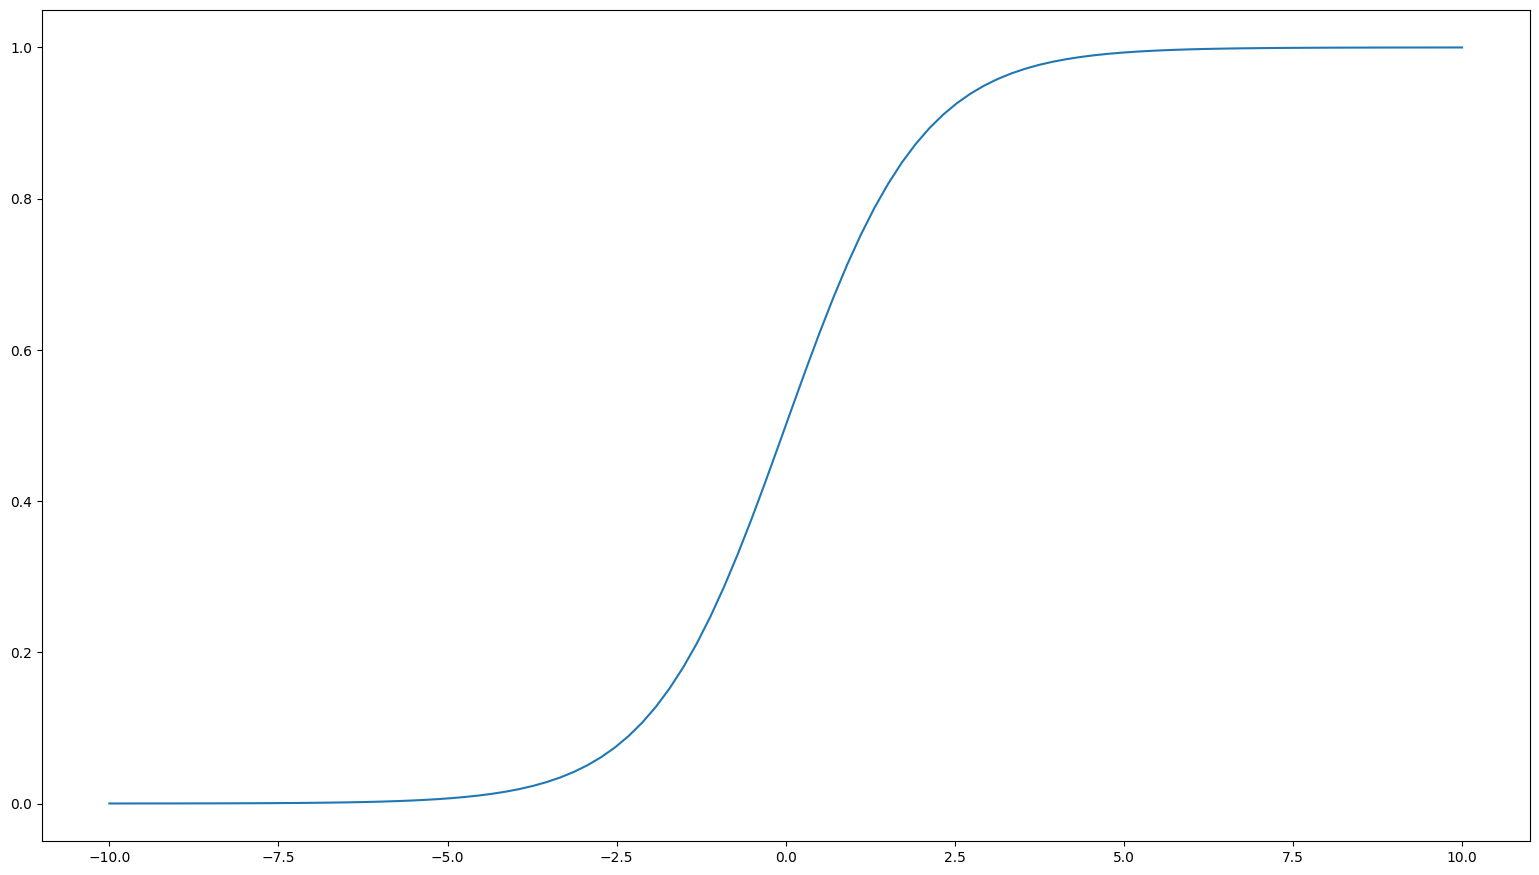
\includegraphics[width=\textwidth]{sigmoid.png}
		\caption{Sigmoid}
		\label{fig:sigmoid}
	\end{figure}
	
	Το logistic regression μοντέλο χρησιμοποιεί την σιγμοειδή (Sigmoid) συνάρτηση Σχ.~\ref{fig:sigmoid} η οποία είναι $\sigma(x) = \frac{1}{1+\exp(-x)}$. Ο αλγόριθμος εκτιμάει την πιθανότητα $\hat{p}=\sigma(X^T\theta)$ και η πρόβλεψη είναι η 
	\begin{equation*}
		\hat{y} = \begin{cases}
			0, &\hat{p}<0.5\\
			1, &\hat{p}\geq 0.5
		\end{cases}
	\end{equation*}
	
	H ensemble μέθοδος λοιπόν εκτελείται σε δύο βήματα. 
	\begin{itemize}
		\item Αρχικά παίρνουμε ένα κομμάτι των δεδομένων για εκπαίδευση και το χωρίζουμε σε δύο υποσύνολα ξένα μεταξύ τους έστω $A$ και $B$
		\item Στη συνέχεια εκπαιδεύουμε τα βασικά μοντέλα στο σύνολο $A$ χωρίς να δουν καθόλου το σύνολο $B$. Αυτό γίνεται για να μην υπάρχει διαρροή πληροφορίας ανάμεσα στα μοντέλα και στο logistic regression.
		\item Έπειτα κάνουμε προβλέψεις στο σύνολο $B$ με τα βασικά μοντέλα και φτιάχνουμε ένα σύνολο $B'$. Έτσι το σύνολο μας αποτελείται από στοιχεία τα οποία έχουν ως διαστάσεις τις προβλέψεις των βασικών μοντέλων.
		\item Τέλος εκπαιδεύουμε το logistic regressor στα στοιχεία του $B'$ δίνοντάς του ταυτόχρονα και τις πραγματικές ετικέτες τους (για αυτό το λόγο στην τεχνική αυτή μιλάμε για ημι-επιβλεπόμενη μάθηση).
	\end{itemize}
	Τελικά το logistic regression θα έχει μάθει να βασίζεται στις προβλέψεις των βασικών μοντέλων. Ωστόσο κρατώντας ξεχωριστά την εκπαίδευση των βασικών μοντέλων και την εκπαίδευση του logistic regression καταφέρνουμε ουσιαστικά να δώσουμε στις προβλέψεις κάθε βασικού μοντέλου ένα βάρος. Συνδυαστικά δηλαδή στο τέλος αν ένα μοντέλο δεν είναι τόσο αξιόπιστο, το logistic regression δεν θα λαμβάνει πολύ την άποψη του σε αντίθεση με την προηγούμενη μέθοδο που κάθε μοντέλο είχε την ίδια αντιμετώπιση με τα υπόλοιπα (δίνοντας βάρος 1 σε όλα).
	
	Η ανωμαλία τελικά προκύπτει από την πιθανότητα που εξάγεται μετά την πρόβλεψη σύμφωνα με αυτό που δείξαμε παραπάνω. Δηλαδή ότι υπολογίζεται κάτω από 0.5 είναι φυσιολογικό σημείο ενώ ότι υπολογίζεται πάνω από 0.5 είναι ανώμαλο σημείο. Ανάλογα την περίπτωση θα μπορούσαμε να πειράξουμε το φράγμα του 0.5 για να μετακινήσουμε το όριο απόφασης. Αυτό θα μας έδινε περισσότερα False Positives ή False Negatives αν μειώναμε ή αυξάναμε το φράγμα. Για παράδειγμα αν πρόκειται για την αντιμετώπιση νοσημάτων σε έναν πληθυσμό θα θέλαμε ιδανικά να μην χαρακτηρίσει το μοντέλο μας κάτι φυσιολογικό ενώ στην πραγματικότητα δεν είναι. Στο παράδειγμα που δώσαμε ένα χαμηλό φράγμα θα ταίριαζε καλύτερα διότι είναι πολύ επιβλαβές να περάσει κάτι επικίνδυνο. Επιπλέον με την ανθρώπινη συμμετοχή θα μπορούσαν να ελέγχονται οι ανωμαλίες (δεδομένου ότι είναι λίγες) και να αποφασίζεται τελικά αν ήταν ανωμαλία ή όχι από τον άνθρωπο. Αντίθετα εάν έχουμε ένα ηλεκτρονικό κατάστημα και οι ανωμαλίες εκεί είναι κακόβουλοι χρήστες τότε με ένα πολύ χαμηλό φράγμα να κάναμε δύσχρηστο το σύστημά μας το οποίο θα είχε ως αποτέλεσμα την απομάκρυνση του κόσμου.
	
	\section{Feature Bagging}
	
	H μέθοδος αυτή έχει προταθεί από τους Lazarevic και Kumar \cite{lazarevicKumar2005Featurebagging} ως μία μέθοδος ανίχνευσης ανωμαλιών σε χρονοσειρές πολλών διαστάσεων. Οι συγγραφείς κάνουν αναφορά σε αλγορίθμους οι οποίοι προσπαθούν να ανιχνεύσουν ανωμαλίες σε δεδομένα πολύ μεγάλων διαστάσεων ενώ ταυτόχρονα θεωρούν ότι είναι άσκοπο να γίνεται μία τέτοια προσπάθεια διότι η σημασία της ομοιότητας (ή της απόστασης) χάνει το νόημά της όσο αυξάνεται ο αριθμός των διαστάσεων. Λόγω του μεγάλου πλήθους τον διαστάσεων τα δεδομένα είναι πολύ μακρυά μεταξύ τους. Αυτό σημαίνει ότι όσο μεγαλώνουν οι διαστάσεις τόσο πιο πολύ απομακρύνονται τα σημεία το ένα από το άλλο και τόσο όλα τα σημεία απομονώνονται που τελικά θεωρούνται όλα ανωμαλίες. Έτσι προτείνεται η μέθοδος Feature Bagging η οποία παίρνει ένα υποσύνολο των διαστάσεων ώστε να αποφύγει το φαινόμενο αυτό. 
	
	\begin{figure}[h]
		\begin{subfigure}[b]{0.49\textwidth}
			\centering
			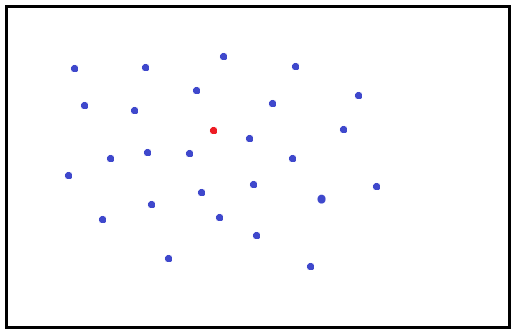
\includegraphics[width=\textwidth]{featurebaggingA.png}
			\caption{Η ανωμαλία δεν ξεχωρίζει από τα δεδομένα}
			\label{fig:featurebaggingA}
		\end{subfigure}
		\hfill
		\begin{subfigure}[b]{0.49\textwidth}
			\centering
			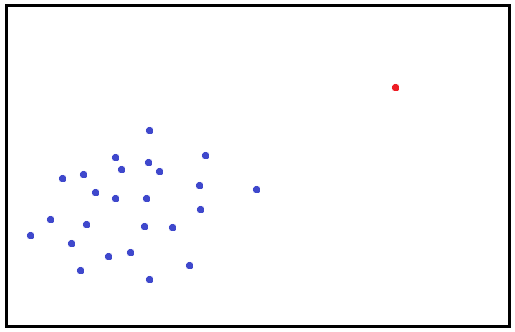
\includegraphics[width=\textwidth]{featurebaggingB.png}
			\caption{Η ανωμαλία ξεχωρίζει από τα δεδομένα}
			\label{fig:featurebaggingB}
		\end{subfigure}
		\caption{Δύο διαφορετικές προβολές των δεδομένων σε δύο διαστάσεις}
		\label{fig:featurebaggingAB}
	\end{figure}
	
	Από την άλλη αν θεωρήσουμε ότι οι περισσότερες διαστάσεις εισάγουν θόρυβο στο σύνολό μας, τότε είναι πιο πιθανό να βρεθούν οι ανωμαλίες μέσα από ένα υποσύνολο των διαστάσεων. Έτσι λοιπόν ο αλγόριθμος αυτός μπορεί να χρησιμοποιηθεί ώστε να μπορέσει να εντοπίσει τις ανωμαλίες κοιτάζοντας κάποιες από τις διαστάσεις και όχι όλες. Στο Σχ.~\ref{fig:featurebaggingAB} βλέπουμε αυτή ακριβώς τη λογική, στην πρώτη εικόνα φαίνεται ότι δεν μπορούμε να ξεχωρίσουμε την ανωμαλία από τα υπόλοιπα δεδομένα, στη δεύτερη εικόνα όμως, βλέπουμε μία προβολή των δεδομένων σε δύο διαστάσεις όπου η ανωμαλία απομονώνεται.
	
	Είναι γνωστό ότι οι βασικοί αλγόριθμοι στις ensemble τεχνικές πρέπει να είναι ικανά μοντέλα αλλά και να έχουν μια διαφορετικότητα μεταξύ τους ώστε να μπορέσουν να συνθέσουν ένα αποδοτικό ensemble μοντέλο. Η ικανότητα των μοντέλων φυσικά παίζει σημαντικό ρόλο, αλλά και η διαφορετικότητα διότι αν τα μοντέλα είναι διαφορετικά τότε δεν θα κάνουν τα ίδια λάθη. Το οποίο σημαίνει ότι ένα λάθος που κάνει ένα μοντέλο θα καλύπτεται από τα υπόλοιπα. Με αυτή τη μέθοδο πετυχαίνουμε επιπλέον να δώσουμε διαφορετικά σύνολα δεδομένων στα μοντέλα, ως εκ τούτου κάθε μοντέλο αποκτάει ιδιαίτερα χαρακτηριστικά. Έτσι ο αλγόριθμος αυτός πετυχαίνει να διαφοροποιεί τα βασικά τους μοντέλα. Ο κλασικός αλγόριθμος bagging δεν καταφέρνει να δώσει ένα αποδοτικό ensemble από βασικούς αλγόριθμους που βασίζονται στα τοπικά χαρακτηριστικά των δεδομένων. Αυτό διότι τέτοιοι αλγόριθμοι δεν είναι ευαίσθητοι σε δειγματοληπτικές μεθόδους. Ωστόσο με τον feature bagging πετυχαίνουμε να διαφοροποιηθούμε από τον κλασικό bagging στο γεγονός ότι αντί να επιλέγουμε σημεία, επιλέγουμε features, στο οποίο είναι πολύ ευαίσθητοι αυτοί οι αλγόριθμοι, εφόσον η επιλογή των features παίζει σημαντικό ρόλο στον υπολογισμό αποστάσεων.
	
	Η διαδικασία για την υλοποίηση αυτής της μεθόδου είναι η εξής: 
	
	\begin{itemize}
		\item Αρχικά παίρνουμε ως δεδομένο ένα σύνολο δεδομένων $\mathcal{S} = \left\{ X_1, X_2,...X_n \right\}$ όπου $X_i\in\mathbb{R}^d$, με $d$ να είναι το πλήθος των διαστάσεων των $X_i$.
		\item Στο πρώτο βήμα της διαδικασίας επιλέγουμε το πλήθος των βασικών αλγόριθμων που θέλουμε να χρησιμοποιήσουμε. Εμείς εδώ έχουμε επιλέξει όλοι οι αλγόριθμοι να έχουν την ίδια αρχιτεκτονική. Έστω $T$ το πλήθος τους, για κάθε έναν από αυτούς εκτελούμε τα επόμενα βήματα.
		
		\begin{itemize}
			
			\item Επιλέγουμε έναν τυχαίο αριθμό $N_t$ από μία ομοιόμορφη κατανομή ανάμεσα στο $\lfloor d \rfloor$ και $(d-1)$. Εδώ το $t$ συμβολίζει τον $t-\text{οστό}$ αλγόριθμο.
			\item Στη συνέχεια επιλέγουμε χωρίς επανάθεση τυχαία $N_t$ features και δημιουργούμε ένα σύνολο από features $\mathcal{F}$
			\item Εκπαιδεύουμε τον αλγόριθμο εντοπισμού ανωμαλιών $\text{Alg}_t$ στα δεδομένα κρατώντας μόνο τα χαρακτηριστικά $\mathcal{F}$.
			\item και παίρνουμε για κάθε σημείο το σκορ ανωμαλίας του αλγόριθμου $t$ $\text{AnomalyScore}_t$
		\end{itemize}
		\item Τελικά για κάθε σημείο έχουμε $T$ σκορ ανωμαλίας (ένα για κάθε αλγόριθμο), \\ $\text{AnomalyScore}_1, \text{AnomalyScore}_2,...,\text{AnomalyScore}_T$ \\ και επιλέγουμε το τελικό σκορ ανωμαλίας εφαρμόζοντας μία συνάρτηση συλλογής. Δηλαδή \\ $\text{AnomalyScore} = \text{Agg}(\text{AnomalyScore}_1, \text{AnomalyScore}_2,...,\text{AnomalyScore}_T)$.
	\end{itemize}
	
	Η επιλογή της συνάρτηση συλλογής παίζει και αυτή ένα ρόλο στην απόδοση του αλγόριθμου. Μία πολύ γνωστή είναι η Βreadth-First η οποία επιλέγει το στοιχείο με το μεγαλύτερο σκορ του πρώτου αλγόριθμου σαν ανωμαλία, στη συνέχει επιλέγει το μεγαλύτερο σκορ του δεύτερου αλγόριθμου σαν ανωμαλία εώς ότου φτάσει στον τελευταίο αλγόριθμο. Έπειτα πηγαίνει στο δεύτερο μεγαλύτερο στοιχείο του τελευταίου αλγόριθμου και το επιλέγει σαν ανωμαλία και εκτελεί το ίδιο μέχρι να γυρίσει στον πρώτο. Η διαδικασία αυτή γίνεται εώς ότου φτάσουμε ένα συγκεκριμένο αριθμό/ποσοστό ανωμαλιών. Ο τρόπος αυτός αν και είναι πολύ δημοφιλής έχει την εξής αδυναμία, θα βρίσκει πάντα ανωμαλίες ακόμα και αν το σύνολο δεδομένων έχει ελάχιστες καμία, ή ακόμα και αν τα σκορ ανωμαλίας είναι πολύ μικρά, μέχρι να πετύχει τον απαιτούμενο αριθμό. Άλλες συναρτήσεις είναι είναι ο μέσος όρος και το άθροισμα. Εμείς εδώ για τα πειράματά μας έχουμε επιλέξει το majority voting το οποίο χρησιμοποιείται και από τους Random Forest. Τελικά μετά την επιλογή ενός φράγματος έχουμε τον εντοπισμό των ανωμαλιών.
	
	\section{Feature Bagging with Rotation}
	Η μέθοδος η οποία προτείνουμε ως μια καλή λύση στον εντοπισμό ανωμαλιών για χρονοσειρές πολλών μεταβλητών είναι μία γενίκευση της προηγούμενης μεθόδου. Η ιδέα έχει προκύψει από τη γνωστή μέθοδο κατηγοριοποίησης Rotation Forest \cite{Rotation2006Forest} η οποία επεκτείνει τα Random Forest. Ωστόσο δεν έχει υλοποιηθεί κάτι παρόμοιο στο πλαίσιο του εντοπισμού ανωμαλιών σε χρονοσειρές πολλών μεταβλητών (τουλάχιστον κατά την δική μας έρευνα).
	
	Για να περιγράψουμε τη μέθοδο αυτή θα πρέπει πρώτα να κάνουμε μια περιγραφή του αλγόριθμου PCA. Ο PCA (Principal Component Analysis) είναι ένας αλγόριθμος γνωστός στη βιβλιογραφία για τη μείωση των διαστάσεων \cite{han2012mining}. Έστω $n$ η διαστάσεις τότε ο αλγόριθμος προσπαθεί να βρει $k\leq n$ $n\text{-διάστατα}$ διανύσματα τα οποία είναι ορθογώνια μεταξύ τους και ταυτόχρονα περιγράφουν/αντιπροσωπεύουν τα υπόλοιπα δεδομένα. Στη συνέχεια τα δεδομένα προβάλλονται στο χώρο που δημιουργούν αυτά τα διανύσματα έτσι προκύπτει μία αναπαράσταση των δεδομένων σε έναν χώρο λιγότερων διαστάσεων χωρίς να χάνεται πληροφορία. Η διαδικασία είναι η εξής:
	
	\begin{enumerate}
		\item Αρχικά τα δεδομένα κανονικοποιούνται. Η κανονικοποίηση των δεδομένων βοηθάει στο να μην επιτρέψει τις πολύ υψηλές τιμές να κυριαρχήσουν και να επηρεάσουν το αποτέλεσμα.
		\item Για κάθε διάσταση υπολογίζεται η μέση τιμή.
		\item Στη συνέχεια υπολογίζεται ο πίνακας συσχέτισης (covariance matrix) για όλες τις διαστάσεις. Δηλαδή $\text{COV}(X,Y) = \frac{1}{m} \cdot \mathlarger{\sum}\limits_{i=1}^{m}(X-\mu_X)(Y-\mu_Y) $
		\item Έπειτα υπολογίζονται τα ιδιοδιανύσματα και οι ιδιοτιμές του προηγούμενου πίνακα. Δηλαδή $\text{det}(A-\lambda I) = 0$. Τα διανύσματα αυτά λέγονται και Principal Components ενώ οι τιμές αναπαριστούν τη "σημαντικότητα".
		\item Bάζουμε σε φθίνουσα σειρά τα διανύσματα ανάλογα με τις ιδιοτιμές. Δηλαδή πρώτα μπαίνει το διάνυσμα με τη μεγαλύτερη ιδιοτιμή, μετά αυτό με την αμέσως επόμενη μεγαλύτερη ιδιοτιμή κοκ. Τα διανύσματα που επιλέγονται είναι τα $k$ πρώτα.
		\item Τέλος παίρνουμε τον πίνακα με τα ιδιοδιανύσματα και πολλαπλασιάζουμε τον ανάστροφο του, με τον αρχικό πίνακα δεδομένων ώστε να γίνει η μετατροπή, άρα:
		\[
		\begin{pmatrix}
			\text{new data}
		\end{pmatrix}
		=
		\begin{pmatrix}
			p_1 & ... & p_k
		\end{pmatrix} ^ T
		\begin{pmatrix}
			\text{data}
		\end{pmatrix}		
		\]
	\end{enumerate}
	Έτσι λοιπόν καταφέρνουμε να μειώσουμε τις διαστάσεις από $n$ σε $k$. Αν λοιπόν κρατήσουμε όλα τα ιδιοδιανύσματα και δεν αφήσουμε κανένα απέξω είναι σαν να στρέφουμε τους άξονες των δεδομένων. Αυτή η ιδέα δίνει τη δυνατότητα στο μοντέλο να δει τα δεδομένα από άλλη "οπτική" γωνία επιτρέποντάς του να αυξήσει την απόδοσή του. Επιπλέον χρησιμοποιείται το Feature Bagging ώστε να έχουμε όλα τα πλεονεκτήματα που είδαμε προηγουμένως. Αρχικά επιλέγουμε τυχαία ένα υποσύνολο από το σύνολο των Features στη συνέχεια εφαρμόζεται ο αλγόριθμος PCA σε αυτό το υποσύνολο. Παίρνουμε τα νέα δεδομένα και εκπαιδεύουμε έναν βασικό αλγόριθμο. Αυτό γίνεται για κάθε βασικό αλγόριθμο που πρόκειται να συνθέσει το ensemble μοντέλο. Στο τέλος μαζεύονται όλα τα αποτελέσματα και εφαρμόζεται μια συνάρτηση συλλογής. Παρακάτω δίνουμε αναλυτικά τη διαδικασία που ακολουθεί ο αλγόριθμος.
	
	Έστω $\mathcal{X}$ μεγέθους $N$ το σύνολο δεδομένων που διαθέτουμε για να κάνουμε την εκπαίδευση του μοντέλου. Τα στοιχεία του $\mathcal{X}$ έχουν $n$ διαστάσεις οπότε ο πίνακας των δεδομένων, έστω $A$, είναι διάστασης $N\times n$. Έστω $D$ το σύνολο των Features και $L$ το πλήθος τον αλγορίθμων που θα χρησιμοποιηθούν. Για κάθε βασικό αλγόριθμο έχουμε:
	\begin{itemize}
		\item  Επιλέγουμε έναν τυχαίο αριθμό $F_l$ από μία ομοιόμορφη κατανομή ανάμεσα στο $\lfloor n \rfloor$ και $(n-1)$. Εδώ το $l$ συμβολίζει τον $l-\text{οστό}$ αλγόριθμο.
		\item Στη συνέχεια επιλέγουμε χωρίς επανάθεση τυχαία $N_t$ features και δημιουργούμε ένα σύνολο από features $F\subseteq D$ και παίρνουμε μόνο αυτά τα features για τα δεδομένα μας.
		\item Επιλέγουμε ένα τυχαίο αριθμό $K$ και χωρίζουμε το σύνολο $F$ σε $K$ υποσύνολα. Τα υποσύνολα αυτά μπορεί να είναι ξένα ή και όχι. Για να αυξήσουμε όμως τη διαφορετικότητα ανάμεσα στους βασικούς αλγόριθμους επιλέγουμε να είναι ξένα. Έτσι τα δεδομένα κάθε υποσυνόλου αποτελείται από $M=n/K$ features.
		\item Επιλέγουμε ένα ποσοστό του συνόλου $\mathcal{X}$. Στο επόμενο βήμα θα εξηγήσουμε γιατί.
		\item Πάνω σε αυτά τα υποσύνολα εφαρμόζουμε το PCA και αποθηκεύουμε τους συντελεστές των principal components, έστω $a_{l,k}^{1},...a_{l,k}^{M}$, όπου με $k$ συμβολίζουμε το $k\text{-οστό}$ υποσύνολο από τα $K$. Στο προηγούμενο βήμα έχουμε επιλέξει ένα ποσοστό επί του συνόλου. Αυτό έγινε για ενισχύσουμε τη διαφορετικότητα ανάμεσα στους συντελεστές σε περίπτωση που τυχαία επιλεγούν ίδια features ανάμεσα στους βασικούς αλγόριθμους. Έτσι ακόμα και ίδιες επιλογές να γίνουν από δύο βασικούς αλγόριθμους οι συντελεστές θα είναι διαφορετικοί, και τελικά θα πετύχουμε τη διαφορετικότητα που θα θέλαμε.
		\item Από το προηγούμενο βήμα παράγουμε έναν πίνακα στροφής για τον βασικό αλγόριθμο $l$: 
		\[
		R_l = 
		\begin{pmatrix}
			a_{l,1}^{1},...a_{l,1}^{M} & [0] & \cdots & [0] \\
			[0] & a_{l,k}^{1},...a_{l,k}^{M} & \cdots & [0] \\
			\vdots & \vdots & \ddots & \vdots \\
			[0] & [0] & \cdots & a_{l,K}^{1},...a_{l,K}^{M}
		\end{pmatrix}		
		\]
		\item Στο προηγούμενο βήμα πρέπει να προσέξουμε ότι εφόσον τα K-υποσύνολα έχουν επιλέξει τυχαία τα features τα $a_i$ δεν είναι στη σειρά. Οπότε σε αυτό το βήμα τοποθετούμε με τα $a_i$ με τη σειρά που παρατηρούνται τα αντίστοιχα features. Έστω $R^{\text{ordered}}_l$ o πίνακας με τη σωστή σειρά.
		\item Τελικά παίρνουμε τα νέα δεδομένα πολλαπλασιάζοντας $X^l_\text{new} = X_l R^{\text{ordered}}_l$ όπου $X_l$ είναι τα αρχικά δεδομένα που θα δίναμε στον αλγόριθμο $l$ πριν την εφαρμογή του PCA. Ο αλγόριθμος $l$ εκπαιδεύεται σε αυτά τα δεδομένα.
		\item Σαν τελικό βήμα της διαδικασίας αφού έχουμε εκπαιδεύσει $L$ βασικούς αλγόριθμους, εφαρμόζουμε μία συνάρτηση συλλογής. Εμείς αποφασίσαμε να ακολουθήσουμε το παράδειγμα των Random Forest και να χρησιμοποιήσουμε το Majority Voting.
	\end{itemize}
	Στη διαδικασία αυτή θα παρατηρήσουμε ότι το ποσοστό των στοιχείων που κρατάμε για να πετύχουμε τη διαφορετικότητα ανάμεσα στους βασικούς αλγόριθμους και ο αριθμός $K$ είναι παράμετροι του ensemble.
	
	Ο αλγόριθμος αυτός όπως θα δούμε και παρακάτω φαίνεται να δίνει πολύ καλά αποτελέσματα. Ένα μειονέκτημα που έχει είναι οι πολλές παράμετροι που πρέπει να επιλέξουμε. Ο αλγόριθμος πέρα από τις παραμέτρους των βασικών αλγόριθμων που πρέπει να επιλεχθούν, έχει επιπλέον την παράμετρο $K$ και το ποσοστό των στοιχείων. Επιπλέον το μεγαλύτερο μειονέκτημά του είναι ο μεγάλος χρόνος εκπαίδευσης. Ο χρόνος εκπαίδευσής του εξαρτάται από 2 παράγοντες. Αρχικά έχουμε το χρόνο εκπαίδευσης κάθε βασικού υπο-μοντέλου και μετά έχουμε το χρόνο που χρειάζεται ο PCA ο οποίος είναι εξαιρετικά χρονοβόρος. Έτσι ο χρόνος που χρειάζεται ένα τέτοιο ensemble να εκπαιδευτεί είναι αρκετά μεγάλος.
	
	\section{Stacking Feature Bagging with Rotation Models}
	Όπως είπαμε και πριν στην τεχνική που ονομάζεται Stacking εκπαιδεύονται όλα τα μοντέλα παράλληλα. Με βάση την έξοδο των μοντέλων στο πρώτο βήμα εκπαιδεύεται ένα μετα-μοντέλο. Για την υλοποίηση της τεχνικής αυτής εμείς χρησιμοποιούμε στο πρώτο στάδιο μοντέλα που έχουν κατασκευαστεί από τη μέθοδο Feature Bagging with Rotation και στη συνέχεια χρησιμοποιούμε έναν Logistic Regressor ως μετα-μοντέλο. Η διαδικασία είναι η εξής:
	
	\begin{itemize}
		\item Αρχικά επιλέγουμε ένα υποσύνολο των δεδομένων στο οποίο θα γίνει η εκπαίδευση. Το υποσύνολο αυτό το χωρίζουμε σε δύο υποσύνολα, $A$ και $B$. Στο $A$ θα εκπαιδευτούν τα επιμέρους μοντέλα ενώ στο $B$ θα εκπαιδευτεί το μετα-μοντέλο.
		\item Επιλέγουμε έναν αριθμό $k>1$
		\item Για κάθε βασικό μοντέλο κατασκευάζονται $k_n$ μοντέλα με την τεχνική Feature Bagging with Rotation όπως περιγράψαμε νωρίτερα (όπου $n$ είναι το n-οστό βασικό μοντέλο).
		\item Κάθε μοντέλο εκπαιδεύεται και παράγει ένα score ανωμαλίας.
		\item Με αυτά τα επιμέρους μοντέλα κάνουμε προβλέψεις σε δεδομένα που δεν έχουν εκπαιδευτεί τα μοντέλα δηλαδή στο σύνολο $B$. Έτσι για κάθε σημείο παίρνουμε $k_n*n$ features (χαρακτηριστικά) όπου $k_n$ ο αριθμός που επιλέξαμε στην αρχή και $n$ ο αριθμός των αρχικών μας μοντέλων. Έτσι κατασκευάζεται ένα νέο σύνολο από το το σύνολο δεδομένων $B$, έστω $B'$ και για κάθε στοιχείο του έχουμε ότι $b_i = (SA_{k_n,n})_{k_n,n} \in \mathbb{R}^{k_n \times n}$, όπου με $SA$ συμβολίζουμε το σκορ ανωμαλίας που έχει δώσει το $k_n$-οστό μοντέλο το οποίο έχει παραχθεί από το n-οστό βασικό μοντέλο μέσω της τεχνικής Feature Bagging with Rotation.
		\item Στο σύνολο $B'$ εφαρμόζουμε επιβλεπόμενη μάθηση εκπαιδεύοντας έναν Logistic Regressor.
	\end{itemize}
	Αυτή η μέθοδος συνδυάζει όλα τα παραπάνω και το αποτέλεσμα είναι να πάρουμε ένα πολύ ισχυρό μοντέλο όπως θα δούμε και παρακάτω. Η αδυναμία αυτής της τεχνικής είναι ότι διατηρεί όλες τις δυσκολίες από τις παραπάνω τεχνικές και ο χρόνος εκπαίδευσης είναι κατά πολύ μεγαλύτερος.
	
	\section{Αρχιτεκτονικές, Υπερπαράμετροι και Μεθοδολογία}
	
	Η εκπαίδευση για κάθε μοντέλο γίνεται σε κάθε σύνολο δεδομένων ξεχωριστά όπως και η πρόβλεψη. Όλα τα μοντέλα εκπαιδεύονται στα ίδια δεδομένα. Τα τελικά αποτελέσματα περιλαμβάνουν τις επιδόσεις ως προς όλα τα σύνολα δεδομένων. Επίσης έχουμε βγάλει αποτελέσματα και για τα βασικά μοντέλα ώστε να μπορεί να γίνει η σύγκριση μεταξύ τους. Η εκπαίδευση είναι χωρίς-επίβλεψη (εκτός από τις τεχνικές που περιλαμβάνουν έναν Logistic Regressor που το μοντέλο εκπαιδεύεται με μερική-επίβλεψη) οπότε κανένα μοντέλο δεν γνωρίζει την πληροφορία "anomaly". Η πληροφορία "anomaly" χρησιμοποιείται στο τέλος ώστε να υπολογίσουμε την απόδοση κάθε αλγόριθμου. Οι αρχιτεκτονικές και οι παράμετροι που χρησιμοποιούνται στα απλά μοντέλα εφαρμόζονται και στα μοντέλα που συνθέτουν τις ensemble τεχνικές. Τέλος στα δεδομένα δεν γίνεται κάποια προεπεξεργασία εκτός από κάποιου είδους κανονικοποίησης και δεν εφαρμόζεται η τεχνική του "ανακατέματος" (shuffling) διότι αυτό θα αφαιρούσε από τα δεδομένα μας την έννοια της χρονικής σειράς. Για να συγκρίνουμε τους αλγόριθμους υπολογίζεται το συνολικό F1 σκορ και το συνολικό AUC (ως προς όλα τα δεδομένα) για τον κάθε αλγόριθμο ενώ ταυτόχρονα παρέχουμε και τον confusion πίνακα.
	
	Έστω ότι τα σύνολα δεδομένων (κάθε σύνολο είναι μία χρονοσειρά πολλών μεταβλητών) μπορεί να αναπαρασταθεί με $(t_0, t_1,....t_n)$  Το σύνολο εκπαίδευσης κάθε συνόλου δεδομένων είναι από τη στιγμή $t_0$ έως τη στιγμή $t_{399}$ και το σύνολο του τεστ είναι $(t_{400}, t_{401},...t_n)$. Στις περιπτώσεις που έχει χρησιμοποιηθεί ο Logistic Regressor το σύνολο εκπαίδευσης των επιμέρους μοντέλων αποτελείται από τα σημεία $(t_0, t_1,....t_{399})$, το σύνολο εκπαίδευσης με ημι-επιβλεπόμενη μάθηση του Logistic Regressor αποτελείται από τα σημεία $(t_{400}, t_{401},...t_{599})$ και τα υπόλοιπα σημεία χρησιμοποιούνται σαν τεστ (Το μέσο μέγεθος των χρονοσειρών είναι περίπου ~1100 χρονικές στιγμές). Τα βασικά μοντέλα που επιλέξαμε είναι Autoencoder, Convolutional Autoencoder, LSTM, LSTM Autoencoder και LSTM Variational Autoencoder και στο Σχ.~\ref{fig:plot_model_architecture_model} μπορούμε να δούμε τις αρχιτεκτονικές τους.
	
	\begin{figure}[H]
		\begin{subfigure}[b]{0.3\textwidth}
			\centering
			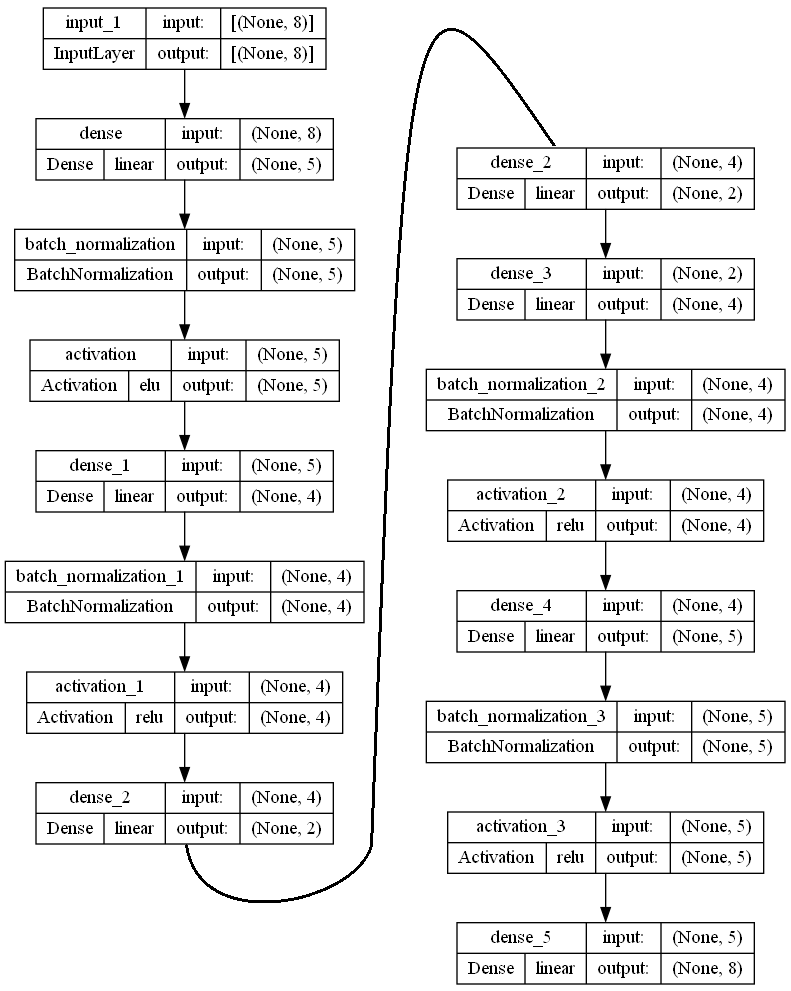
\includegraphics[width=\textwidth]{plot_model_autoencoder_model_c.png}
			\caption{Autoencoder}
			\label{fig:plot_model_autoencoder_model}
		\end{subfigure}
		\hfill
		\begin{subfigure}[b]{0.3\textwidth}
			\centering
			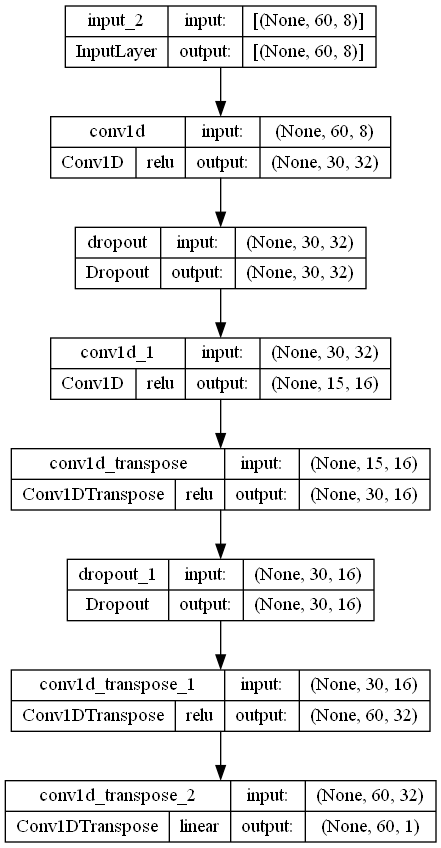
\includegraphics[width=\textwidth]{plot_model_conv_ae_model.png}
			\caption{Convolutional Autoencoder}
			\label{fig:plot_model_conv_ae_model}
		\end{subfigure}
		\hfill
		\begin{subfigure}[b]{0.3\textwidth}
			\centering
			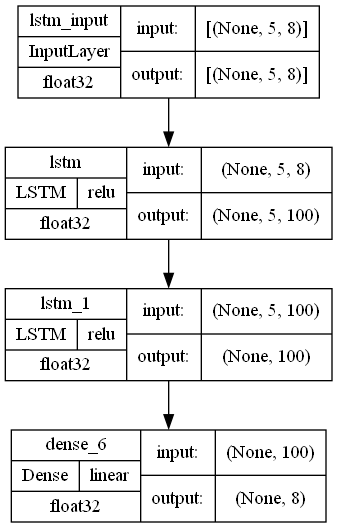
\includegraphics[width=\textwidth]{plot_model_lstm_model.png}
			\caption{LSTM}
			\label{fig:plot_model_lstm_model}
		\end{subfigure}
		\hfill
		\begin{subfigure}[b]{0.3\textwidth}
			\centering
			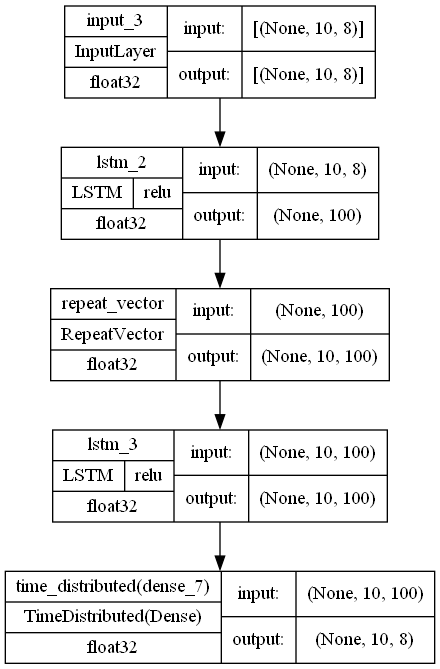
\includegraphics[width=\textwidth]{plot_model_lstm_ae_model.png}
			\caption{LSTM Autoencoder}
			\label{fig:plot_model_lstm_ae_model}
		\end{subfigure}
		\hfill
		\begin{subfigure}[b]{0.5\textwidth}
			\centering
			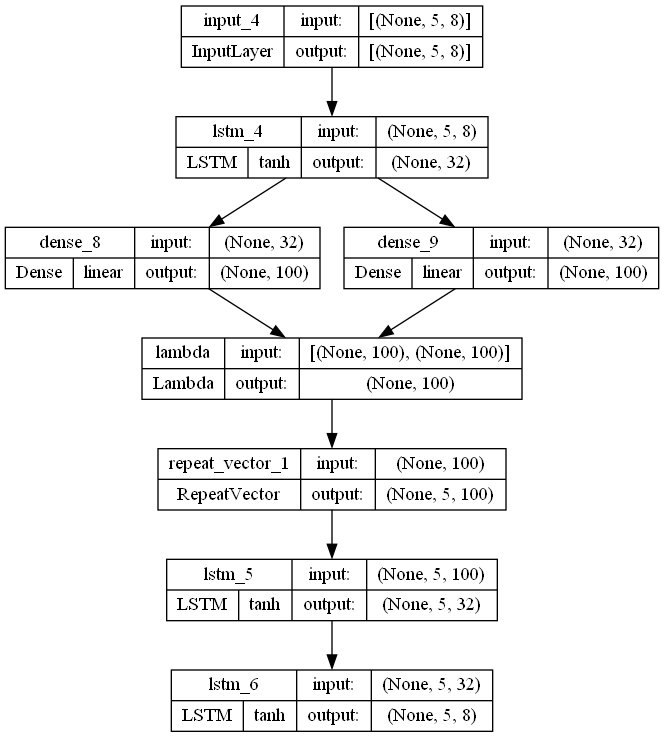
\includegraphics[width=\textwidth]{plot_model_lstm_vae_model.png}'
			\caption{LSTM Variational Autoencoder}
			\label{fig:plot_model_lstm_vae_model}
		\end{subfigure}
		
		\caption{Αρχιτεκτονικές Βασικών Μοντέλων}
		\label{fig:plot_model_architecture_model}
	\end{figure}
	
	Το μέγεθος του παραθύρου που χρησιμοποιούμε είναι 60 χρονικές στιγμές για τον Convolutional Autoencoder, 5 για τον LSTM, 10 για τον LSTM Autoencoder και 5 για τον LSTM Variational Autoencoder. Για την τεχνική Feature Bagging χρησιμοποιήσαμε 17 estimators. Για την τεχνική Feature Bagging with Rotation χρησιμοποιήθηκαν 17 estimators, το Κ το θέσαμε 2 και το ποσοστό των δεδομένων που χρησιμοποιήθηκαν για τον αλγόριθμο PCA ήταν στο 75\%. Τέλος στο Stacking των Feature Bagging with Rotation με μετα-μοντέλο έναν Logistic Regressor χρησιμοποιήθηκαν 12 estimators για κάθε μία από τους 5 βασικούς αλγόριθμους όπου οι παράμετροι για κάθε μία από αυτές ήταν K=2 και το ποσοστό στο 80\%. Να θυμίσουμε εδώ ότι οι βασικές τεχνικές και οι τεχνικές Majority Voting και Logistic Regression χρησιμοποιούν όλα τα features ενώ στις υπόλοιπες τεχνικές 
	
	\chapter{Αποτελέσματα}
	\section{Αποτελέσματα}
	Οι παραπάνω τεχνικές εφαρμόστηκαν σε 31 σύνολα δεδομένων τα οποία προσομοιώνουν διαφορετικές καταστάσεις. Για κάθε ένα από αυτά τα σύνολα τα μοντέλα εκπαιδεύονται σε ένα κομμάτι τους και στη συνέχεια κάνουν τις προβλέψεις σε ολόκληρα τα σύνολα. Στο πλαίσιο του εντοπισμού των ανωμαλιών δεν μπορούμε να μετρήσουμε την απόδοση ενός μοντέλου με την κλασική μετρική "Accuracy" η οποία δίνεται από το $\text{Accuracy} = \frac{\text{TP}+\text{TN}}{\text{TP}+\text{FP}+\text{TN}+\text{FN}}$ όπου TP, FP, TN, FN είναι τα True Positives, False Positives, True Negative, False Negatives αντίστοιχα. Οπότε επιλέξαμε να μετρήσουμε τις αποδόσεις με βάση τα F1 score και το AUC (οι ορισμοί δόθηκαν σε προηγούμενο κεφάλαιο). Στη συνέχεια θα δώσουμε τα αποτελέσματα από τις τεχνικές που αναφέραμε ως προς το σύνολο των δεδομένων, πρώτα όμως, θα πρέπει να εξηγήσουμε τι είναι ένας Confusion Πίνακας.
	
	\begin{figure}[h]
		\centering
		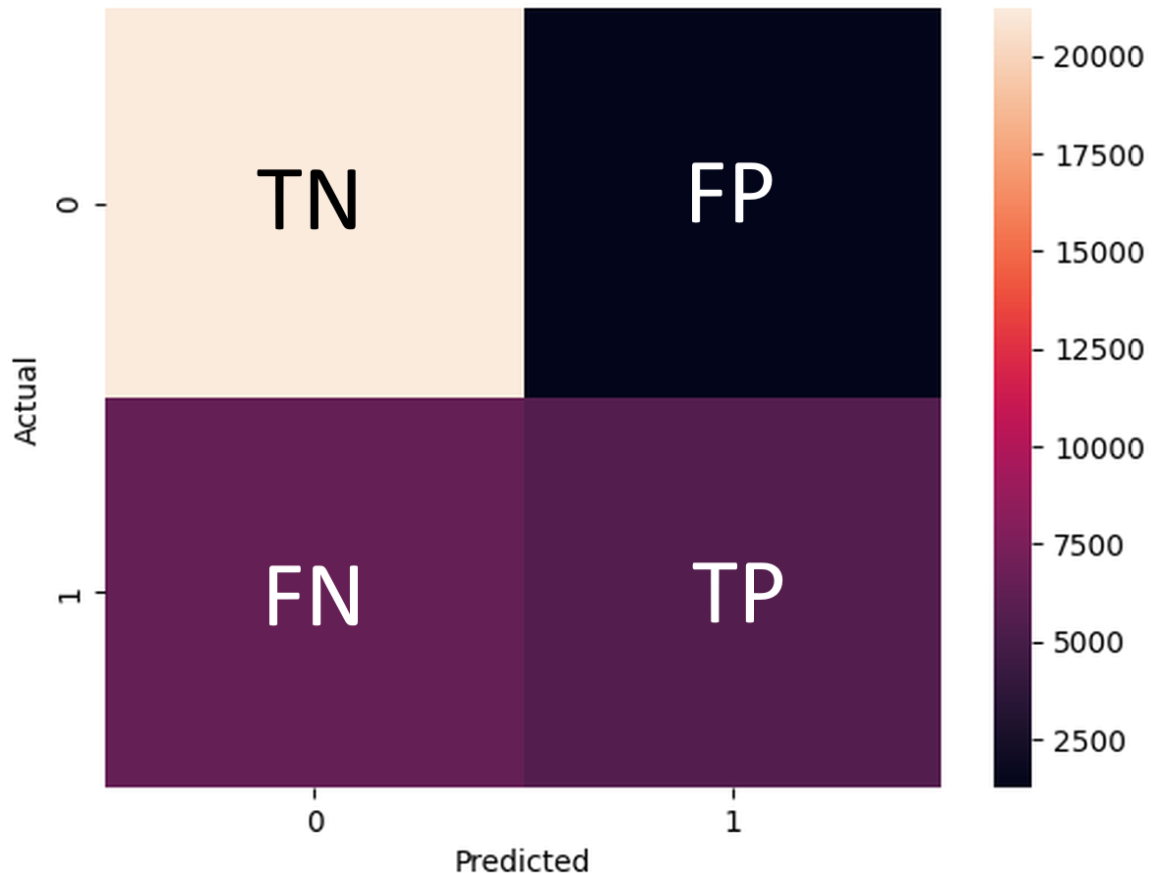
\includegraphics[width=\textwidth/2]{confusionmatrixexplain.png}
		\caption{Confusion Matrix}
		\label{fig:confusionmatrixexplain}
	\end{figure}
	
	Ένας Confusion Πίνακας αποτελείται από 4 περιοχές τα True Positives, True Negative, False Positives και False Negative. Στην αριστερή πλευρά του πίνακα μπορούμε να διαλέξουμε ανάμεσα στα πραγματικά δεδομένα (πάνω γραμμή τα πραγματικά φυσιολογικά σημεία ενώ στην κάτω γραμμή έχουμε έχουμε τα πραγματικά Ανώμαλα δεδομένα). Στην κάτω πλευρά του πίνακα μπορούμε να διαλέξουμε ανάμεσα στις προβλέψεις (στην αριστερή στήλη έχουμε τις προβλέψεις των φυσιολογικών σημείων ενώ στη δεξιά τις προβλέψεις των ανώμαλων σημείων). Στο Σχ.~\ref{fig:confusionmatrixexplain} βλέπουμε έναν confusion matrix όπου αντί για αριθμούς έχουμε σημειώσει σε κάθε περιοχή τι δείχνει. Σημειώνουμε εδώ ότι το ιδανικό μοντέλο θα είχε στις περιοχές των FP και FN τον αριθμό μηδέν.
	
	\begin{figure}[H]
		\centering
		\begin{subfigure}[b]{0.35\textwidth}
			\centering
			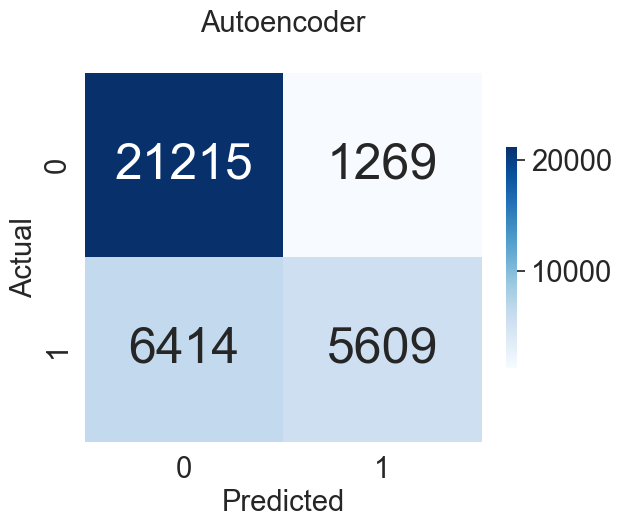
\includegraphics[width=\textwidth]{anomaly_by_autoencoder.png}
			
			\label{fig:anomaly_by_autoencoder}
		\end{subfigure}
		\hfil
		\begin{subfigure}[b]{0.35\textwidth}
			\centering
			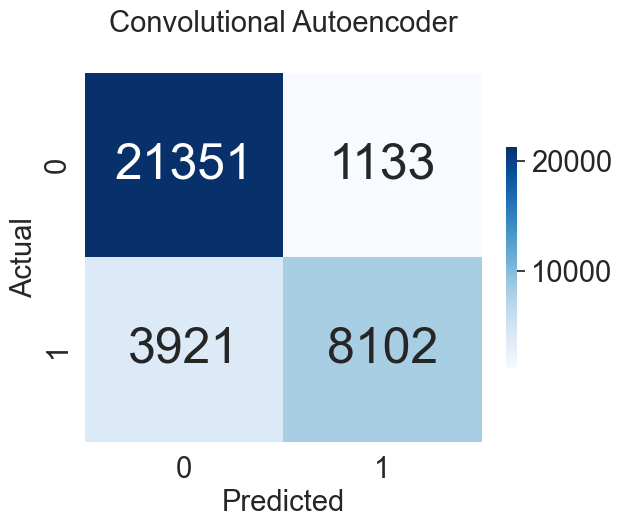
\includegraphics[width=\textwidth]{anomaly_by_conv_ae.png}
			
			\label{fig:anomaly_by_conv_ae}
		\end{subfigure}
		\bigskip
		\begin{subfigure}[b]{0.35\textwidth}
			\centering
			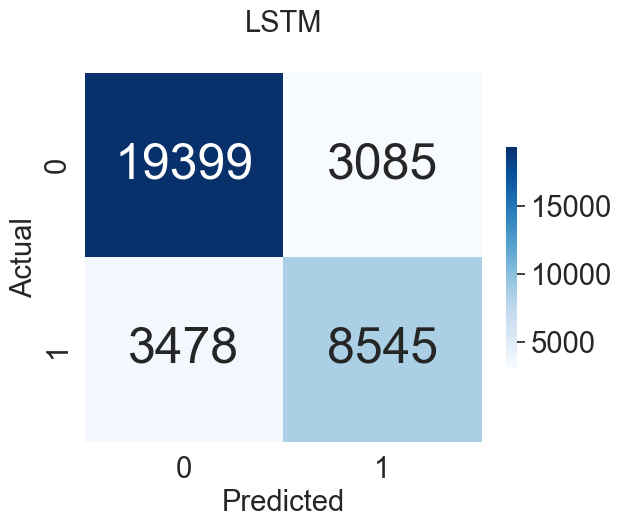
\includegraphics[width=\textwidth]{anomaly_by_lstm.png}
			
			\label{fig:anomaly_by_lstm}
		\end{subfigure}
		\hfil
		\begin{subfigure}[b]{0.35\textwidth}
			\centering
			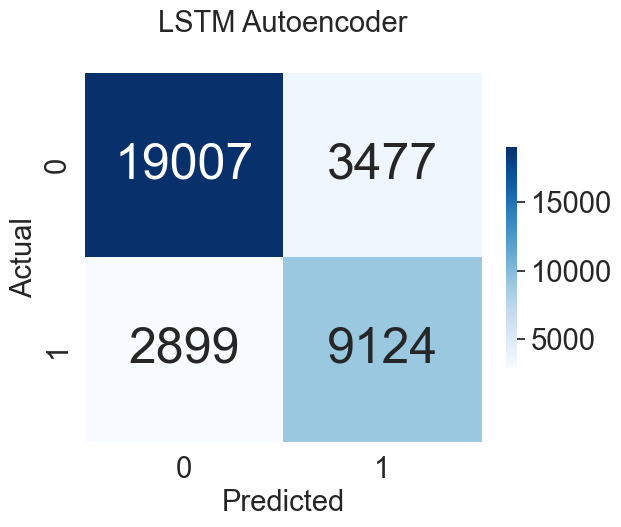
\includegraphics[width=\textwidth]{anomaly_by_lstm_ae.png}
			
			\label{fig:anomaly_by_lstm_ae}
		\end{subfigure}
		\medskip
		\begin{subfigure}[b]{0.35\textwidth}
			\centering
			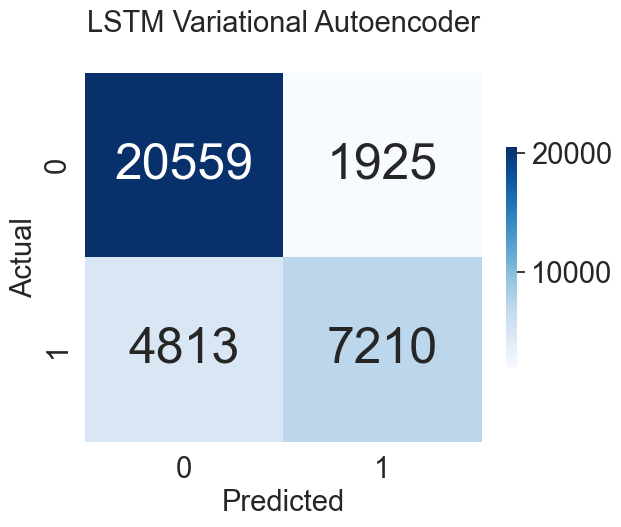
\includegraphics[width=\textwidth]{anomaly_by_lstm_vae.png}
			
			\label{fig:anomaly_by_lstm_vae}
		\end{subfigure}
		\caption{Βασικά Μοντέλα}
		\label{fig:basicmodelsconfusion}
	\end{figure}
	
	Παράλληλα με τις τεχνικές εκπαιδεύσαμε και τα βασικά μοντέλα ώστε να έχουμε ένα μέτρο σύγκρισης στη συνέχεια. Στο Στο Σχ.~\ref{fig:basicmodelsconfusion} βλέπουμε τα αποτελέσματα που είχαν τα βασικά μοντέλα. Παρατηρούμε ότι τα μοντέλα πετυχαίνουν καλές επιδόσεις ειδικότερα ο convolutional autoencoder και ο LSTM autoencoder.
	
	\begin{figure}[H]
		\centering
		\begin{subfigure}[b]{0.35\textwidth}
			\centering
			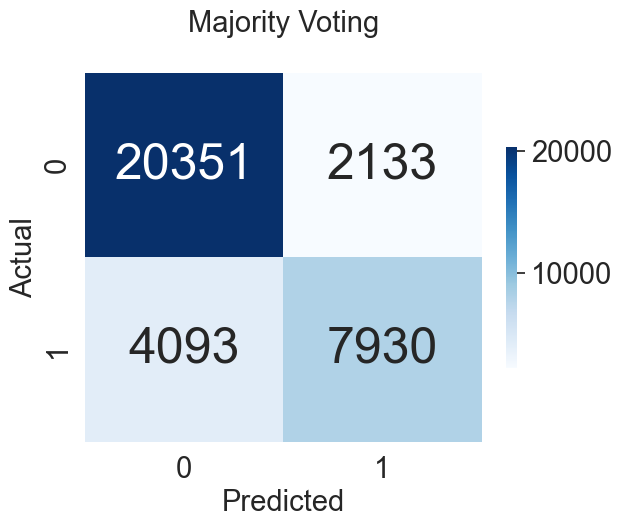
\includegraphics[width=\textwidth]{anomaly_by_voting.png}
			
			\label{fig:anomaly_by_voting}
		\end{subfigure}
		\hfil
		\begin{subfigure}[b]{0.35\textwidth}
			\centering
			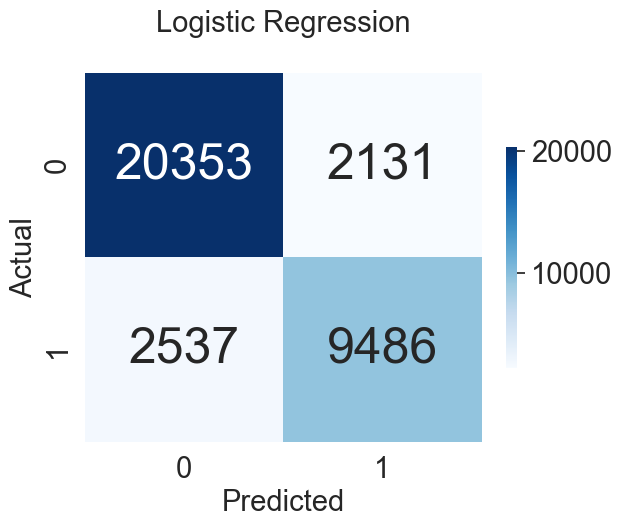
\includegraphics[width=\textwidth]{anomaly_by_logistic_regression.png}
			
			\label{fig:anomaly_by_logistic_regression}
		\end{subfigure}
		\caption{Majority Voting - Logistic Regression}
		\label{fig:majoritylogistic}
	\end{figure}
	
	
	\begin{figure}[H]
		\centering
		\begin{subfigure}[b]{0.35\textwidth}
			\centering
			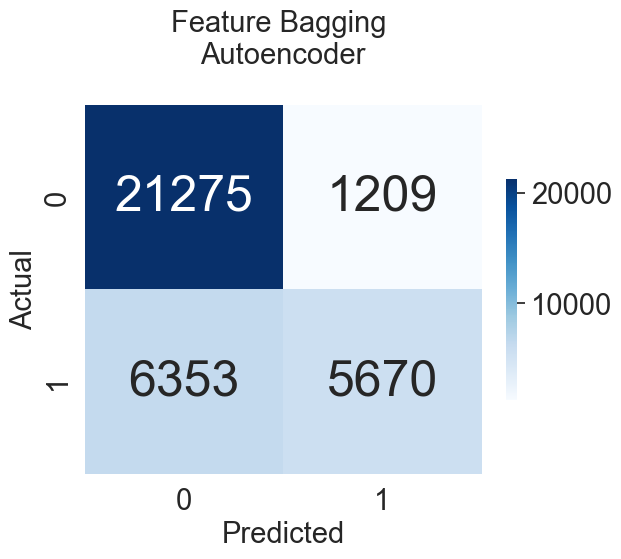
\includegraphics[width=\textwidth]{anomaly_by_ensemble_ensemble_autoencoder.png}
			
			\label{fig:anomaly_by_ensemble_ensemble_autoencoder}
		\end{subfigure}
		\hfil
		\begin{subfigure}[b]{0.35\textwidth}
			\centering
			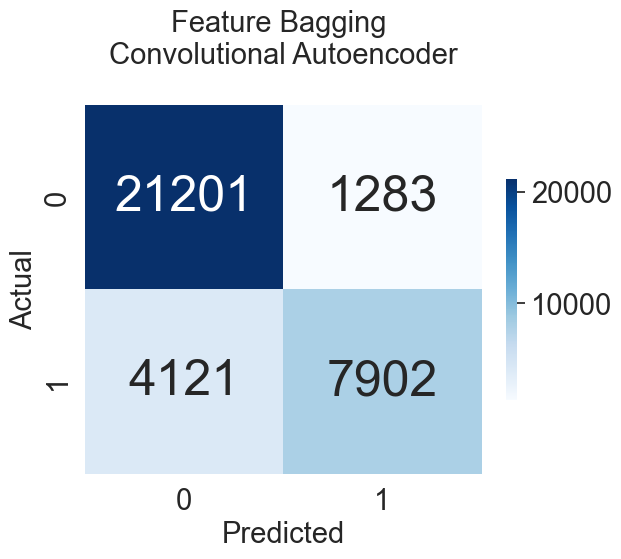
\includegraphics[width=\textwidth]{anomaly_by_ensemble_ensemble_conv_ae.png}
			
			\label{fig:anomaly_by_ensemble_ensemble_conv_ae}
		\end{subfigure}
		\medskip
		\begin{subfigure}[b]{0.35\textwidth}
			\centering
			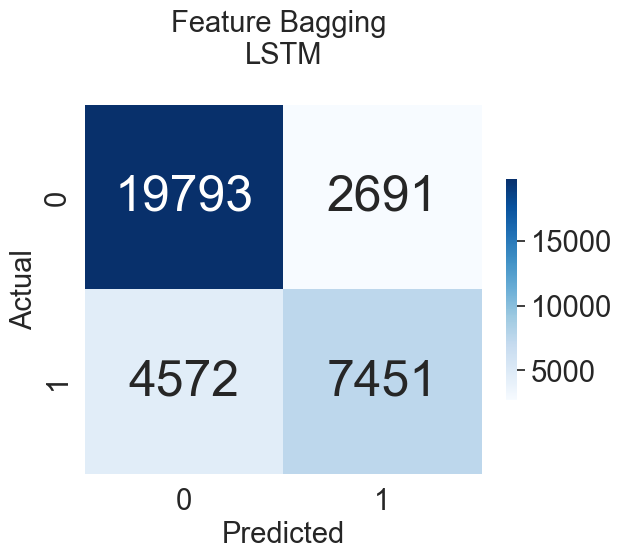
\includegraphics[width=\textwidth]{anomaly_by_ensemble_ensemble_lstm.png}
			
			\label{fig:anomaly_by_ensemble_ensemble_lstm}
		\end{subfigure}
		\hfil
		\begin{subfigure}[b]{0.35\textwidth}
			\centering
			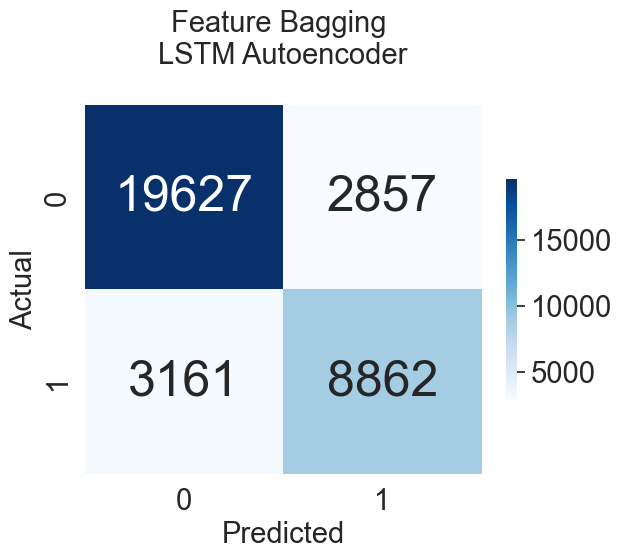
\includegraphics[width=\textwidth]{anomaly_by_ensemble_ensemble_lstm_ae.png}
			
			\label{fig:anomaly_by_ensemble_ensemble_lstm_ae}
		\end{subfigure}
		\medskip
		\begin{subfigure}[b]{0.35\textwidth}
			\centering
			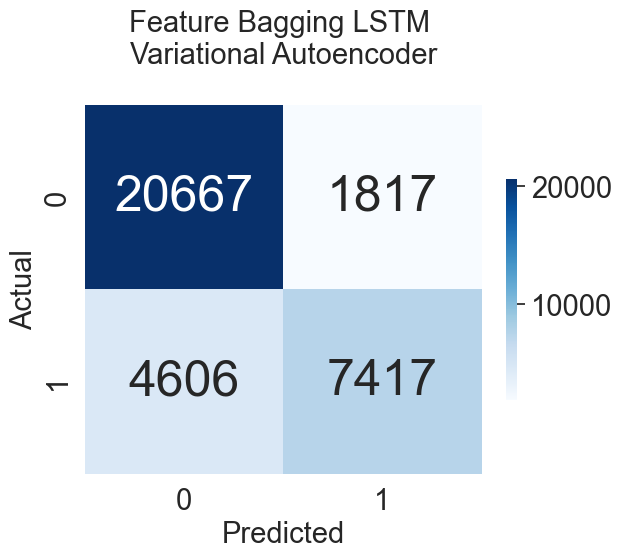
\includegraphics[width=\textwidth]{anomaly_by_ensemble_ensemble_lstm_vae.png}
			
			\label{fig:anomaly_by_ensemble_ensemble_lstm_vae}
		\end{subfigure}
		\caption{Feature Bagging}
		\label{fig:featurebaggingmodelsconfusion}
	\end{figure}
	
	Στη συνέχεια δίνουμε τα αποτελέσματα για τις τεχνικές που αναφέραμε προηγουμένως. Ξεκινάμε με τον Majority Voting και την τεχνική όπου εφαρμόζουμε ημι-επιβλεπόμενη μάθηση με Logistic Regression Σχ.~\ref{fig:majoritylogistic}. Παρατηρούμε ότι και οι δύο αλγόριθμοι είναι πολύ κοντά στα σημεία που δεν είναι ανωμαλίες όμως διαφέρουν στα ανώμαλα σημεία. Όπως βλέπουμε ο Logistic Regression πετυχαίνει καλύτερα αποτελέσματα εκεί.
	
	Στη συνέχεια παρουσιάζουμε τα αποτελέσματα της τεχνικής Feature Bagging Σχ.~\ref{fig:featurebaggingmodelsconfusion}. Παρατηρούμε ότι εδώ ανάλογα με τον βασικό αλγόριθμο που έχει χρησιμοποιηθεί υπάρχει μια ποικιλία στα αποτελέσματα. Στην επόμενη ενότητα θα δούμε μία σύγκριση ανάμεσα σε κάθε βασικό αλγόριθμο και στην τεχνική Feature Bagging που του αντιστοιχεί.
	
	\begin{figure}[H]
		\centering
		\begin{subfigure}[b]{0.35\textwidth}
			\centering
			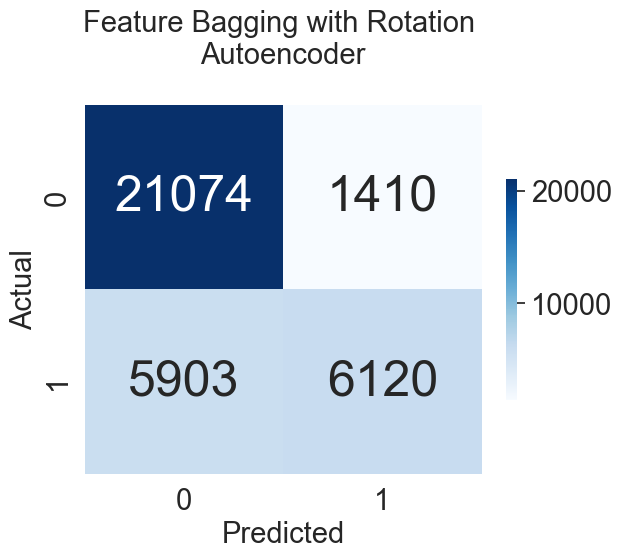
\includegraphics[width=\textwidth]{anomaly_by_ensemble_ensemble_rotation_autoencoder.png}
			
			\label{fig:anomaly_by_ensemble_ensemble_rotation_autoencoder}
		\end{subfigure}
		\hfil
		\begin{subfigure}[b]{0.35\textwidth}
			\centering
			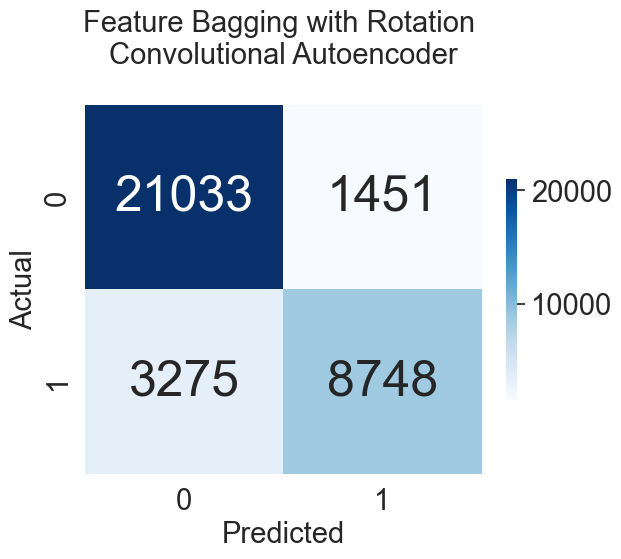
\includegraphics[width=\textwidth]{anomaly_by_ensemble_ensemble_rotation_conv_ae.png}
			
			\label{fig:anomaly_by_ensemble_ensemble_rotation_conv_ae}
		\end{subfigure}
		\medskip
		\begin{subfigure}[b]{0.35\textwidth}
			\centering
			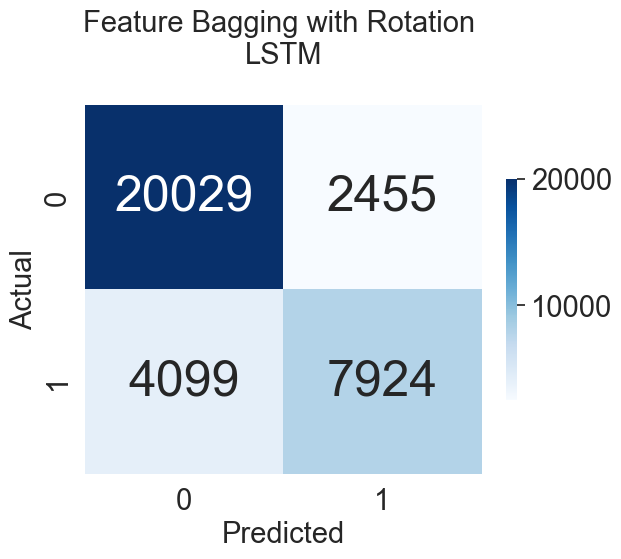
\includegraphics[width=\textwidth]{anomaly_by_ensemble_ensemble_rotation_lstm.png}
			
			\label{fig:anomaly_by_ensemble_ensemble_rotation_lstm}
		\end{subfigure}
		\hfil
		\begin{subfigure}[b]{0.35\textwidth}
			\centering
			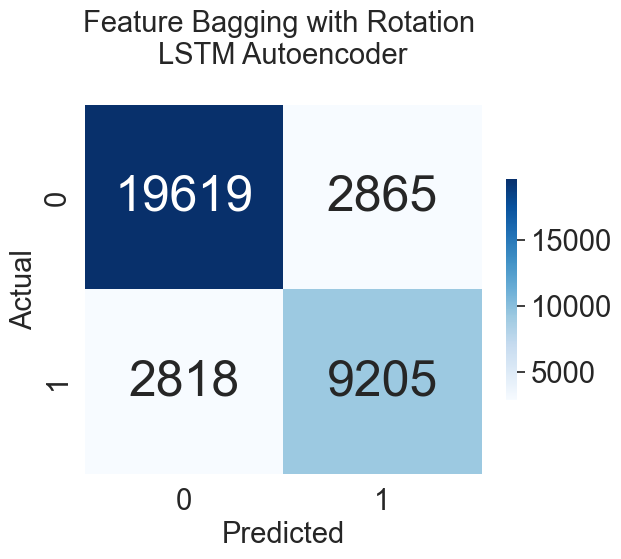
\includegraphics[width=\textwidth]{anomaly_by_ensemble_ensemble_rotation_lstm_ae.png}
			
			\label{fig:anomaly_by_ensemble_ensemble_rotation_lstm_ae}
		\end{subfigure}
		\medskip
		\begin{subfigure}[b]{0.35\textwidth}
			\centering
			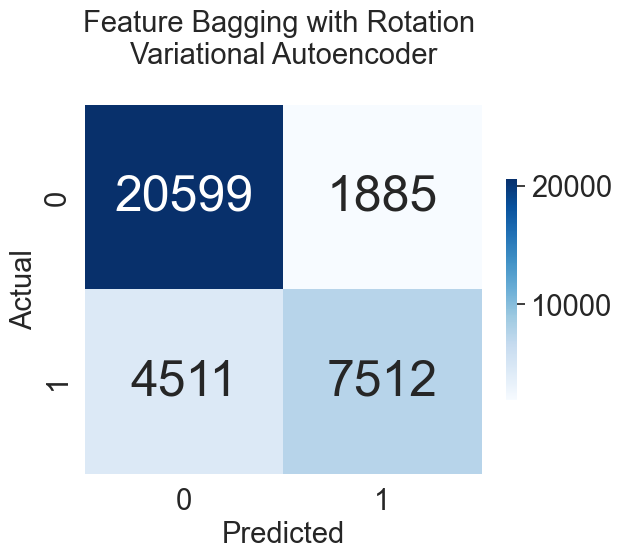
\includegraphics[width=\textwidth]{anomaly_by_ensemble_ensemble_rotation_lstm_vae.png}
			
			\label{fig:anomaly_by_ensemble_ensemble_rotation_lstm_vae}
		\end{subfigure}
		\caption{Feature Bagging with Rotation}
		\label{fig:featurebaggingwithrotationmodelsconfusion}
	\end{figure}
	
	Στο Σχ.~\ref{fig:featurebaggingwithrotationmodelsconfusion} παρουσιάζουμε τα αποτελέσματα της τεχνικής Feature Bagging with Rotation όπου με τη βοήθεια του αλγόριθμου PCA στρίβουμε τους άξονες. Παρατηρούμε και εδώ ότι ανάλογα με τον βασικό αλγόριθμο που έχει χρησιμοποιηθεί υπάρχει μια ποικιλία στα αποτελέσματα.
	
	\begin{figure}[H]
		\centering
		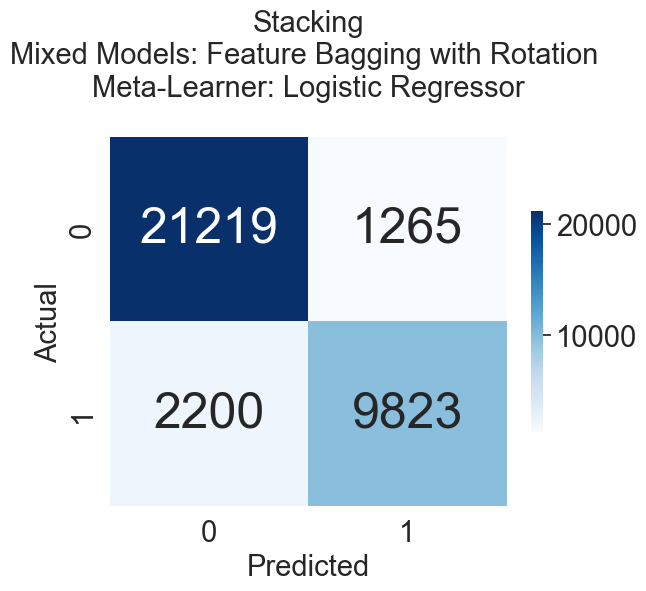
\includegraphics[width=\textwidth/3]{anomaly_by_logistic_regression_mixed_models.png}
		\caption{Stacking, Mixed Models: Feature Bagging with Rotation, Meta-Learner: Logistic Regressor}
		\label{fig:anomaly_by_logistic_regression_mixed_models}
	\end{figure}
	
	Τέλος παραθέτουμε τα αποτελέσματα από το Stacking που χρησιμοποιήσαμε σε μοντέλα κατασκευασμένα από την τεχνική Feature Bagging with Rotation με μετα-μοντέλο έναν Logistic Regressor Σχ.~\ref{fig:anomaly_by_logistic_regression_mixed_models}
	
	\section{Συγκρίσεις}
	
	Στους παρακάτω πίνακες γίνεται μία σύγκριση ανάμεσα στα βασικά μοντέλα και τις τεχνικές. Όπως είπαμε και προηγουμένως χρησιμοποιούμε τις μετρικές F1 score και AUC για να αξιολογήσουμε τα μοντέλα. Με βάση αυτές τις μετρικές παρατηρούμε ότι η τεχνική Feature Bagging δίνει αρκετά καλά αποτελέσματα σε κάποιες περιπτώσεις ενώ η τεχνική Feature Bagging with Rotation κερδίζει σε όλες τις συγκρίσεις εκτός από την περίπτωση που το βασικό μοντέλο είναι ο LSTM. Επιπλέον ο Majority Voting είναι περίπου στη μέση (κάτι που το περιμέναμε εφόσον στηρίζεται στην πλειοψηφία) ενώ ο αλγόριθμος με το Logistic Regression κερδίζει τους βασικούς αλγόριθμους καθώς στηρίζεται στο γεγονός ότι μαθαίνει να κάνει την καλύτερη επιλογή στηριζόμενος στην πρόβλεψη των βασικών. Επιπλέον είναι ο μόνος αλγόριθμος που γνωρίζει έστω και λίγες ετικέτες από τα δεδομένα. Τέλος αξίζει να αναφερθεί ότι δεν μπορούμε να κάνουμε συγκρίσεις μεταξύ των Feature Bagging τεχνικών διότι δεν στηρίζονται στους ίδιους βασικούς αλγόριθμους. Το ίδιο συμβαίνει και με την τεχνική Feature Bagging with Rotation. 
	
	\begin{table}[H]
		\centering
		\resizebox{\textwidth/3*2}{!}{
			\begin{tabular}{|c|c|c|}
				\hline
				Model Title & F1 Score & AUC \\
				\hline
				Feature Bagging with Rotation Autoencoder & 62.59 \% & 72.31 \% \\
				%& 0.6259908965376157 & 0.7231565543080914 \\
				\hline
				Feature Bagging Autoencoder & 59.99 \% & 70.89 \% \\
				% & 0.5999365146545339 & 0.7089122682829209 \\
				\hline
				Autoencoder & 59.35 \% & 70.50 \% \\ 
				% & 0.5935135707105444 & 0.705041181668599 \\
				\hline
			\end{tabular}
		}
		\caption{Autoencoder}
		\label{tab:comptabautoencoder}
	\end{table}
	
	Παρατηρούμε στους αλγόριθμους Autoencoder, LSTM Autoencoder και LSTM Variational Autoencoder ο Feature Bagging έχει καλύτερη επίδοση από το αντίστοιχο βασικό μοντέλο και ο Feature Bagging with Rotation καλύτερη επίδοση από τον Feature Bagging ενώ σε σχέση με τα βασικά μοντέλα η επίδοση βελτιώνεται 2\% Πίνακας~\ref{tab:comptabautoencoder} Πίνακας~\ref{tab:comptablstmautoencoder} Πίνακας~\ref{tab:comptablstmvariationalautoencoder}. Στην περίπτωση του Convolutional Autoencoder το Feature Bagging with Rotation συνεχίζει να έχει καλύτερη επίδοση όμως σε αντίθεση με τα προηγούμενα ο Feature Bagging όχι Πίνακας~\ref{tab:comptablstm}. O μόνος βασικός αλγόριθμος που έχει καλύτερη επίδοση από τις αντίστοιχες εκδόσεις του Feature Bagging και Feature Bagging with Rotation είναι ο LSTM Πίνακας~\ref{tab:comptablstm}.
	
	\begin{table}[H]
		\centering
		\resizebox{\textwidth}{!}{
			\begin{tabular}{|c|c|c|}
				\hline
				Model Title & F1 Score & AUC \\
				\hline
				Feature Bagging with Rotation Convolutional Autoencoder & 78.73 \%  & 83.15 \% \\
				% & 0.7873278732787328 & 0.8315353213255807 \\
				\hline
				Convolutional Autoencoder & 76.22 \% & 81.17 \% \\
				% & 0.7622542101796971 & 0.8117418416723458 \\
				\hline
				Feature Bagging Convolutional Autoencoder & 74.51 \% & 80.00 \% \\
				% & 0.7451904941531498 & 0.8000887446158723 \\
				\hline
			\end{tabular}
		}
		\caption{Convolutional Autoencoder}
		\label{tab:comptabconvolutionalautoencoder}
	\end{table}
	
	\begin{table}[H]
		\centering
		\resizebox{\textwidth/3*2}{!}{
			\begin{tabular}{|c|c|c|}
				\hline
				Model Title & F1 Score & AUC \\
				\hline
				LSTM & 72.25 \% & 78.67 \% \\
				% & 0.7225299116391154 & 0.786756218064105 \\
				\hline
				Feature Bagging with Rotation LSTM & 70.74 \% & 77.49 \% \\
				% & 0.707436835996786 & 0.7749406795813568 \\
				\hline
				Feature Bagging LSTM & 67.23 \% & 75.00 \% \\
				% & 0.6723212271599368 & 0.7500218718102761 \\
				\hline
			\end{tabular}
		}
		\caption{LSTM}
		\label{tab:comptablstm}
	\end{table}
	
	\begin{table}[H]
		\centering
		\resizebox{\textwidth/3*2}{!}{
			\begin{tabular}{|c|c|c|}
				\hline
				Model Title & F1 Score & AUC \\
				\hline
				Feature Bagging with Rotation LSTM Autoencoder & 76.41 \% & 81.90 \% \\ 
				% & 0.7641223591914665 & 0.8190959784678844 \\
				\hline
				Feature Bagging LSTM Autoencoder & 74.65 \% & 80.50 \% \\
				% & 0.7465251453121052 & 0.805009556048233 \\
				\hline
				LSTM Autoencoder & 74.10 \% & 80.21 \% \\
				% & 0.7410656270305394 & 0.8021177568499255 \\
				\hline
			\end{tabular}
		}
		\caption{LSTM Autoencoder}
		\label{tab:comptablstmautoencoder}
	\end{table}
	
	\begin{table}[H]
		\centering
		\resizebox{\textwidth/4*3}{!}{
			\begin{tabular}{|c|c|c|}
				\hline
				Model Title & F1 Score & AUC \\
				\hline
				Feature Bagging with Rotation LSTM Variational Autoencoder & 70.14 \% & 77.04 \% \\
				% & 0.7014005602240897 & 0.770482533233351 \\
				\hline
				Feature Bagging LSTM Variational Autoencoder & 69.78 \% & 76.80 \% \\
				% & 0.6978407112951028 & 0.768043958635707 \\
				\hline
				LSTM Variational Autoencoder & 68.15 \% & 75.70 \% \\
				% & 0.6815388978164287 & 0.7570337503802643 \\
				\hline
			\end{tabular}
		}
		\caption{LSTM Variational Autoencoder}
		\label{tab:comptablstmvariationalautoencoder}
	\end{table}
	
	Παρατηρούμε στους Πίνακες~\ref{tab:comptabautoencoder}-\ref{tab:comptablstmvariationalautoencoder} ότι η τεχνική Feature Bagging with Rotation ανταποκρίνεται καλύτερα σε όλα τα βασικά μοντέλα εκτός από την περίπτωση του LSTM όπου σε αυτή την περίπτωση αποτυγχάνει και η τεχνική Feature Bagging. Εδώ να θυμίσουμε πάλι ότι η εκπαίδευση έγινε με 17 estimators για κάθε περίπτωση, με K=2 και ποσοστό δεδομένων στο 75 \%.
	
	\begin{table}[H]
		\centering
		\resizebox{\textwidth/2}{!}{
			\begin{tabular}{|c|c|c|}
				\hline
				Model Title & F1 Score & AUC \\
				\hline
				Convolutional Autoencoder & 76.22 \% & 81.17 \% \\
				% & 0.7622542101796971 & 0.8117418416723458 \\
				\hline
				LSTM Autoencoder & 74.10 \% & 80.21 \% \\
				% & 0.7410656270305394 & 0.8021177568499255 \\
				\hline
				LSTM & 72.25 \% & 78.67 \% \\
				% & 0.7225299116391154 & 0.786756218064105 \\
				\hline
				Majority Voting & 71.81 \% & 78.23 \% \\
				% & 0.7181019650457303 & 0.7823508489029425 \\
				\hline
				LSTM Variational Autoencoder & 68.15 \% & 75.70 \% \\
				% & 0.6815388978164287 & 0.7570337503802643 \\
				\hline
				Autoencoder & 59.35 \% & 70.50 \% \\
				% & 0.5935135707105444 & 0.705041181668599 \\
				\hline
			\end{tabular}
		}
		\caption{Majority Voting}
		\label{tab:comptabmajorityvoting}
	\end{table}
	
	Ο Majority Voting έχει τοποθετηθεί στη μέση του πίνακα με μικρή διαφορά από το LSTM ενώ παράλληλα έχει πετύχει καλύτερη επίδοση πάνω από 8\% από τον Autoencoder Πίνακας~\ref{tab:comptablstm}. Τέλος ο Logistic Regressor πετυχαίνει καλύτερα αποτελέσματα από όλους τους βασικούς αλγόριθμους Πίνακας~\ref{tab:comptablogreg}
	
	
	\begin{table}[H]
		\centering
		\resizebox{\textwidth/2}{!}{
			\begin{tabular}{|c|c|c|}
				\hline
				Model Title & F1 Score & AUC \\
				\hline
				Logistic Regression & 80.25 \% & 84.71 \% \\
				% & 0.8025380710659897 & 0.8471046321360901 \\
				\hline
				Convolutional Autoencoder & 76.22 \% & 81.17 \% \\
				% & 0.7622542101796971 & 0.8117418416723458 \\
				\hline
				LSTM Autoencoder & 74.10 \% & 80.21 \% \\
				% & 0.7410656270305394 & 0.8021177568499255 \\
				\hline
				LSTM & 72.25 \% & 78.67 \% \\
				% & 0.7225299116391154 & 0.786756218064105 \\
				\hline
				LSTM Variational Autoencoder & 68.15 \% & 75.70 \% \\
				% & 0.6815388978164287 & 0.7570337503802643 \\
				\hline
				Autoencoder & 59.35 \% & 70.50 \% \\
				% & 0.5935135707105444 & 0.705041181668599 \\
				\hline
			\end{tabular}
		}
		\caption{Logistic Regression}
		\label{tab:comptablogreg}
	\end{table}
	
	Τέλος την καλύτερη επίδοση πετυχαίνει ο αλγόριθμος που εφαρμόζουμε το Stacking των Feature Bagging with Rotation με μετα-μοντέλο ένα Logistic Regressor Πίνακας~\ref{tab:comptablogregmixedmodels}
	
	\begin{table}[H]
		\centering
		\resizebox{\textwidth/2}{!}{
			\begin{tabular}{|c|c|c|}
				\hline
				Model Title & F1 Score & AUC \\
				\hline
				Stacking with Logistic Regression & 85.00 \% & 88.03 \% \\
				% & 0.8025380710659897 & 0.8471046321360901 \\
				\hline
				Convolutional Autoencoder & 76.22 \% & 81.17 \% \\
				% & 0.7622542101796971 & 0.8117418416723458 \\
				\hline
				LSTM Autoencoder & 74.10 \% & 80.21 \% \\
				% & 0.7410656270305394 & 0.8021177568499255 \\
				\hline
				LSTM & 72.25 \% & 78.67 \% \\
				% & 0.7225299116391154 & 0.786756218064105 \\
				\hline
				LSTM Variational Autoencoder & 68.15 \% & 75.70 \% \\
				% & 0.6815388978164287 & 0.7570337503802643 \\
				\hline
				Autoencoder & 59.35 \% & 70.50 \% \\
				% & 0.5935135707105444 & 0.705041181668599 \\
				\hline
			\end{tabular}
		}
		\caption{Stacking with Logistic Regression}
		\label{tab:comptablogregmixedmodels}
	\end{table}
	
	
	
	\chapter{Συμπεράσματα}
	\section{Συμπεράσματα και Περαιτέρω επέκταση της εργασίας}
	Στην εργασία αυτή υλοποιήσαμε διάφορες ensemble τεχνικές για την ανίχνευση ανωμαλιών σε χρονοσειρές πολλών μεταβλητών. Το πρόβλημα αυτό έχει προσεγγιστεί από διάφορους αλγόριθμους τόσο από στατιστικές τεχνικές όσο και από Μηχανικής μάθησης και βαθιάς μηχανικής μάθησης μοντέλα. Εμείς πήραμε δεδομένα κάποια βασικά μοντέλα βαθιάς μηχανικής μάθησης και στηριχθήκαμε σε αυτά ώστε να υλοποιήσουμε ensemble τεχνικές ώστε να πετύχουμε ακόμα καλύτερα αποτελέσματα. Τα ensemble μοντέλα που κατασκευάστηκαν αρχικά ήταν ένας Majority Voting ο οποίος είχε μια μέτρια επίδοση και ένας αλγόριθμος με ημι-επιβλεπόμενη εκπαίδευση όπου σαν τελικό μοντέλο χρησιμοποιήθηκε ένας Logistic Regressor. Στη συνέχεια υλοποιήθηκε ένα αλγόριθμος που ονομάζεται Feature Bagging ο οποίος μοιάζει πολύ με την τεχνική που χρησιμοποιείται στους Random Forest. Ο Feature Bagging έδωσε κάποια καλά αποτελέσματα σε κάποιες περιπτώσεις έναντι των βασικών μοντέλων. Στη συνέχεια από μια ιδέα που προέρχεται από τους Rotation Forest χρησιμοποιήθηκε ο PCA πάνω στον Feature Bagging με αποτέλεσμα να παραχθεί ένας αλγόριθμος οποίος στις περισσότερες περιπτώσεις είχε καλύτερη επίδοση από όλα τα παραπάνω και από τους βασικούς αλγόριθμους. Τέλος χρησιμοποιήθηκε μία stacking τεχνική με επιμέρους μοντέλα κατασκευασμένα από την τεχνική Feature Bagging with Rotation και μετα-μοντέλο έναν Logistic Regressor όπου πιάσαμε την καλύτερη επίδοση από όλες τις προηγούμενες τεχνικές. Οι ensemble τεχνικές είναι γνωστό ότι βελτιώνουν κατά πολύ τις επιδόσεις και λύνουν αρκετά προβλήματα. Τα παραπάνω αποτελέσματα μας δείχνουν ότι μπορούν να βοηθήσουν πάρα πολύ και στην ανίχνευση ανωμαλιών. Με τις ensemble μεθόδους μπορούμε να ξεπεράσουμε αρκετά τα απλά μοντέλα και να παραχθεί ένα υπερ-μοντέλο το οποίο θα εντοπίζει αρκετά αξιόπιστα τις ανωμαλίες. Ειδικότερα ο αλγόριθμος Feature Bagging with Rotation μπόρεσε να έχει 2\% καλύτερη επίδοση από τα βασικά μοντέλα σε κάποιες περιπτώσεις ενώ ο Feature Bagging όταν ήταν καλύτερος από ένα απλό μοντέλο είχε καλύτερη επίδοση περίπου 1\% σε μία περίπτωση ενώ στις άλλες δύο είχε λιγότερο από 1\%. Τελικά όταν εφαρμόσαμε το Stacking πετύχαμε περίπου 10 \% καλύτερη επίδοση σε σχέση με τα βασικά μοντέλα.
	
	Από τα παραπάνω μπορούμε να πούμε ότι αξίζει η περαιτέρω επέκταση της εργασίας και η προσπάθεια ανίχνευσης ανωμαλιών με ensemble τεχνικές καθώς φαίνεται ότι τα ensemble μοντέλα μπορούν να δώσουν λύσεις. Οι περισσότερες από τις τεχνικές χρειάζονται κάποια συνάρτηση συγκέντρωσης των αποτελεσμάτων οπότε θα μπορούσε αυτό να αποτελέσει αντικείμενο έρευνας ώστε με την κατάλληλη συνάρτηση να μπορούν να συνδυαστούν τα αποτελέσματα των βασικών μοντέλων πιο αποτελεσματικά. Οι Shahzad και Lavesson έχουν κάνει μία έρευνα \cite{shahzad2013comparative} στην οποία ερευνούν παραλλαγές του Majority Voting και φαίνεται ότι ο Majority Voting πετυχαίνει καλύτερα αποτελέσματα σαν αλγόριθμος αλλά θα ήταν ενδιαφέρον να ερευνηθεί αν μπορούν οι παραλλαγές να χρησιμοποιηθούν σαν συναρτήσεις επιλογής των τεχνικών που περιγράψαμε και αν μπορούν να δώσουν καλύτερα αποτελέσματα.
	
	Επιπλέον τα σύνολα δεδομένων αποτελούνται από λίγα features, δηλαδή οι χρονοσειρές πολλών μεταβλητών αποτελούνται από λίγες μεταβλητές (συνολικά 8), αυτό σημαίνει ότι οι αλγόριθμοι αυτοί θα μπορούσαν να ερευνηθούν και σε παραπάνω διαστάσεις. Όσο αυξάνονται οι διαστάσεις τόσο πιο πολύ χάνεται το νόημα της ανωμαλίας κάτι που κάνει δύσκολο τον εντοπισμό, όμως πιστεύουμε ότι οι αλγόριθμοι αυτοί θα μπορούσαν να αντεπεξέλθουν πολύ καλά ειδικότερα οι αλγόριθμοι Feature Bagging και Feature Bagging with Rotation οι οποίοι μπορούν να εκμεταλλευτούν τις πολλές διαστάσεις.
	
	Ένα άλλο κομμάτι σημαντικό για αυτούς τους αλγόριθμους είναι το κομμάτι της ταχύτητας. Παρατηρήσαμε ότι όσο αυξάνεται η πολυπλοκότητα τόσο αυξάνεται και ο χρόνος που χρειάζονται τα μοντέλα για να εκπαιδευτούν. Αυτό σημαίνει ότι είναι αδύνατον να πάμε σε πολύ μεγάλο αριθμό βασικών μοντέλων. Ο μεγάλος αριθμός βασικών μοντέλων θα μας έδινε τη δυνατότητα να έχουμε καλύτερες επιδόσεις όμως κάτι τέτοιο ήταν αδύνατον δεδομένου του χρόνου που έπαιρνε για παράδειγμα ένα Feature Bagging with Rotation να εκπαιδευτεί. Έτσι λοιπόν αξίζει να διερευνηθεί παραπάνω το πώς θα μπορούσε αυτό να γίνει σε πολύ λιγότερο χρόνο ώστε να μπορέσει ένας τέτοιος αλγόριθμος να αποτελείται από πολλά μικρά βασικά μοντέλα.
	
	
	
	\bibliographystyle{ieeetr}
	\bibliography{mybib}
	%\bibliographystyle{abbrv}
	%\bibliographystyle{acm}
	%\bibliographystyle{alpha}
	%\bibliographystyle{apalike}
	%\bibliographystyle{ieeetr}
	%\bibliographystyle{plain}
	%\bibliographystyle{unsrt}
	
\end{document}

